% !TEX root = main_ilyi.tex

% for pdfLaTeX
% \pdfoutput=1

\documentclass[11pt]{article}

% Change "review" to "final" to generate the final (sometimes called camera-ready) version.
% Change to "preprint" to generate a non-anonymous version with page numbers.
\RequirePackage{lib}

% Standard package includes
\RequirePackage{times}
\RequirePackage{latexsym}

% For proper rendering and hyphenation of words containing Latin characters (including in bib files)
\RequirePackage[T1]{fontenc}

% This assumes your files are encoded as UTF8
\RequirePackage[utf8]{inputenc}

\RequirePackage{microtype}

\RequirePackage{inconsolata}

\RequirePackage{graphicx}
\RequirePackage{amsmath}
\RequirePackage{multirow}
\RequirePackage{booktabs}
\RequirePackage{amssymb}
\RequirePackage{hyperref}
\RequirePackage{subfig}

\RequirePackage{algorithm}
\RequirePackage{algpseudocode}
\RequirePackage{verbatim}

% If the title and author information does not fit in the area allocated, uncomment the following
%
%\setlength\titlebox{<dim>}
%
% and set <dim> to something 5cm or larger.

\title{Multimodal Information Extraction of Supermarket Leaflets}

\author{Ilyesse Hettenbach\textsuperscript{}, Gabriel Schurr\textsuperscript{} \\
HKA, Karlsruhe, Germany \\
\texttt{\{heil1012, scga1011\}@h-ka.de} \\
\href{https://github.com/ilyii/leaflets}{https://github.com/ilyii/leaflets}
}


\begin{document}
\maketitle
\begin{abstract}
Supermarket leaflets are a valuable source of information for consumers, offering insights into product deals, discounts, and promotions. However, extracting structured information from these leaflets is a challenging task due to their unstructured nature and layout variability. In this work, we present an intelligent system for extracting, structuring, and utilizing information from supermarket leaflets in a digital format. Our approach leverages advanced computer vision, Optical Character Recognition (OCR), and language models to detect and extract deals from these leaflets. We propose a modular pipeline for deal detection and information extraction, develop an interactive application for browsing and comparing deals, and introduce Leaflet-IE, a benchmark dataset for evaluating information extraction models. Our system aims to enhance the digital transformation of supermarket leaflets, providing consumers with a more efficient and data-driven shopping experience.
\end{abstract}

\section{Introduction}

\subsection{Motivation}
When one thinks of a paper-heavy country, Germany is likely to come to mind. The country's affinity for printed materials is deeply ingrained in its culture, with activities such as browsing through supermarket leaflets serving as a familiar ritual for many individuals. These leaflets have long been an essential medium for consumers to plan their purchases, discover special offers, and compare prices.
The rapid advancement of digital technology is transforming consumer behavior. While some individuals still find browsing through physical leaflets a nostalgic and even relaxing experience, younger generations are increasingly turning to digital alternatives for their shopping needs. The modern shopper expects convenience, efficiency, and instant access to information, yet the digital transformation of supermarket leaflets in Germany lags significantly behind, even despite the existence of applications that centralize digital versions of these leaflets. The majority of these digital leaflets are plain documents, failing to leverage the full potential of interactivity, searchability and intelligent recommendation systems. 

Furthermore, while price comparison websites and applications have become commonplace for electronics, fashion and travel, the grocery sector remains an overlooked frontier. Consumers are often left navigating multiple supermarket websites or manually cross-referencing prices to find the best deals. This is often a tedious and inefficient process. A comprehensive digital ecosystem that integrates grocery price comparisons, personalized discounts and AI-driven shopping assistants could bridge this gap and act as a workaround, offering an enhanced, data-driven shopping experience and a tool that allows consumers to create a dynamic shopping list, track price trends over time, and receive real-time updates on the best deals.

\subsection{Problem Statement}
The primary objective of this research is to develop an intelligent system for extracting, structuring, and utilizing information from supermarket leaflets in a digital format. Given a set of supermarket leaflets $\mathbf{L} = \{L_1, L_2, ..., L_n\}$, where each $L_i$ contains a set ofproduct deals $\{p_j\}_{j=1}^{m} \in P_{L_i}$, the goal is to extract and normalize these attributes to enable efficient querying and comparison across multiple supermarket chains.

Each product deal $p_j$ is represented by a set of attributes $\{y_1, y_2, ..., y_k\} \subset p_j$, where each attribute $y_k$ represents a specific entity. Common attributes include the name and brand of the product, the original and deal prices, the unit (e.g., weight, volume), and the product image. The challenge lies in detecting and separating deals from the leaflet, extracting structured information from the detected deals, normalizing the extracted information to ensure consistency and comparability, and validating the extracted information to ensure accuracy. 

To enable advanced applications such as the abovementioned, one has to tackle different challenges, such as:
\begin{enumerate}
    \item Gathering a diverse set of supermarket leaflets from various retailers.
    \item Detecting and separating deals $p$ from the leaflet $L$.
    \item Extracting structured information from the detected deals.
    \item Normalizing the extracted information to ensure consistency and comparability.
    \item Validating the extracted information to ensure accuracy.
    \item Storing the extracted information in a structured format for efficient querying and comparison.
    \item Developing an interactive application for browsing and comparing deals across multiple supermarket chains.
\end{enumerate}

Therefore, a function $f: \mathcal{L} \to \mathcal{D}$ has to be designed, that maps a set of leaflets $\mathcal{L}$ to a set of structured deals $\mathcal{D}$, where each deal $d \in \mathcal{D}$ is represented by a set of attributes $\{y_1, y_2, ..., y_k\}$.


\subsection{Contributions}
To build this mapping, this work presents the conducted research and the practical result of a comprehensive approach to digitalizing and structuring supermarket leaflet information by leveraging advanced computer vision, Optical Character Recognition (OCR), and language models, depicted in \figref{fig:overview}. A \emph{modular pipeline} is proposed that encompasses deal detection, information extraction and normalization to transform raw leaflet data into structured, actionable insights.

\begin{figure*}
    \centering
    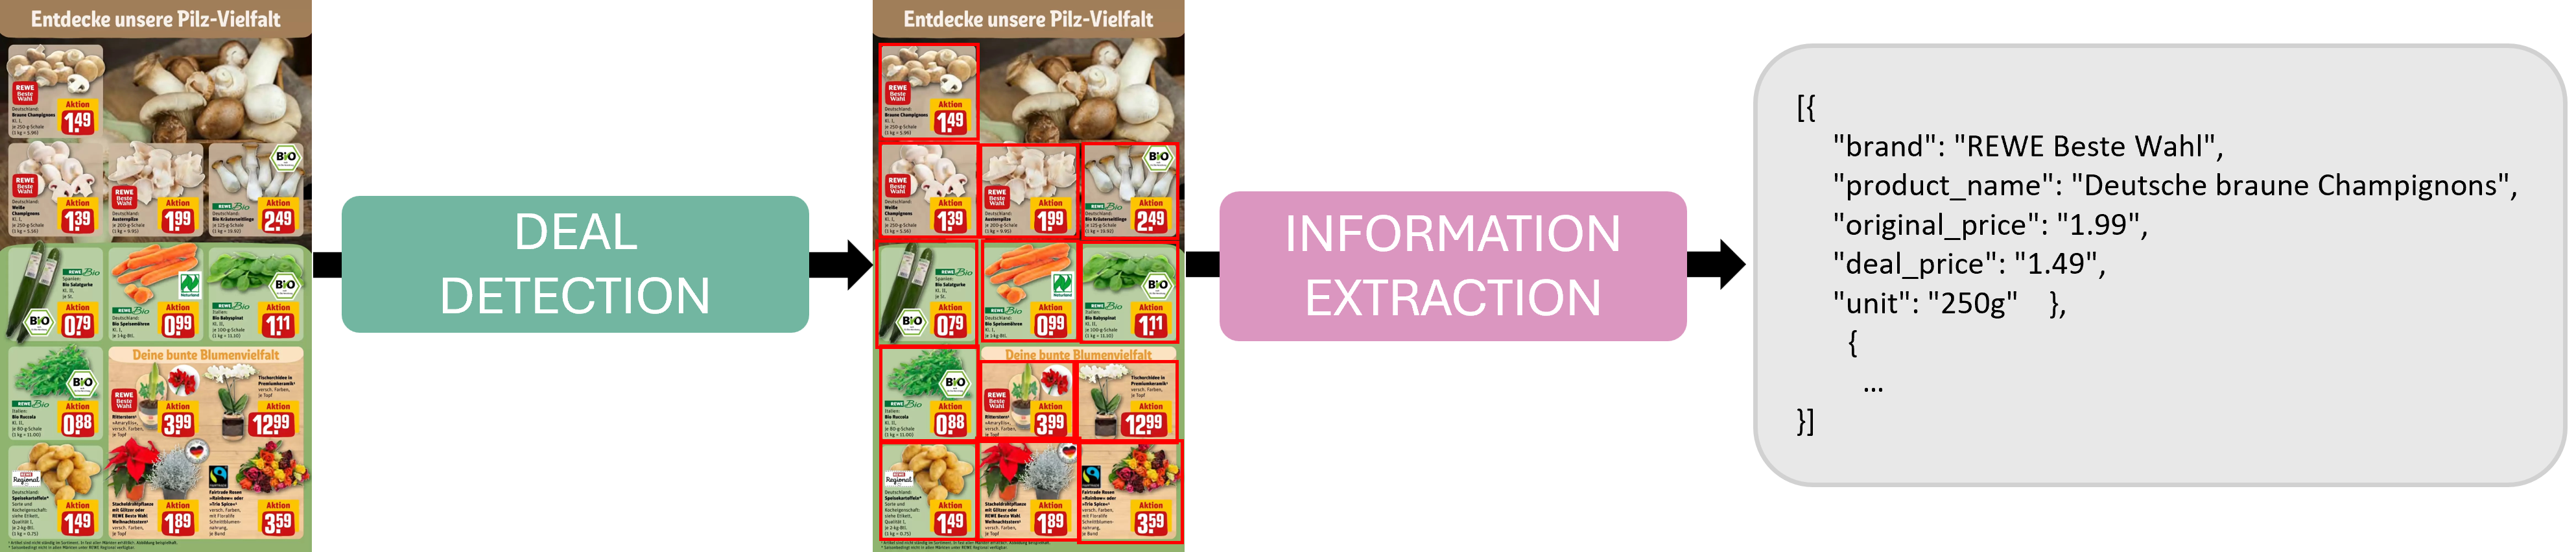
\includegraphics[width=0.8\linewidth]{figures/overview.png}
    \caption{Overview of the proposed approach to digitalizing and structuring supermarket leaflet information.}
    \label{fig:overview}
\end{figure*}

To enhance usability, an \emph{interactive application} is developed that allows consumers to browse, filter, and compare deals across multiple supermarket chains. In addition, a feature allows an entire leaflet to be uploaded and the entire pipeline to be run in order to examine the deals in detail. This application serves as a proof of concept for the proposed system and demonstrates its practical utility.

To facilitate research and development in this domain, \emph{Leaflet-IE}, an end-to-end benchmark dataset for information extraction from supermarket leaflets, is introduced. This dataset stands as a valuable resource for evaluating and comparing different models and approaches in the field.

\subsection{Structure}
This work is structured to systematically address supermarket deal detection and information extraction, beginning with a scientific overview of related works in \secref{sec:related_works}. The nature of supermarket leaflet data is analyzed in \secref{sec:leaflets_data}, formalizing challenges such as layout variability, OCR noise, and multimodal fusion. Deal detection is covered in \secref{sec:deal_detection}, detailing an own dataset creation, instance segmentation model selection, and experimental results for identifying promotional content. Information extraction is extended in \secref{sec:information_extraction}, detailing an own benchmark dataset construction, popular architectural approach and their performance evaluation for extracting structured product and pricing information. Thereafter, the proposed interactive application is introduced in \secref{sec:application}, outlining its features, design, and user interface. The work concludes with a summary of contributions and future research directions in \secref{sec:conclusion}.


\section{Related Works}
\label{sec:related_works}

\indent{\textbf{Supermarket Leaflet Analysis}.}
The field of supermarket leaflet analysis has evolved to tackle key challenges such as product classification, promotion identification, and customer interaction. Recent studies have leveraged AI-driven techniques to enhance efficiency and accuracy in this domain. For instance, cite{ladwig2023} explore fine-grained product classification in leaflet advertisements, while \cite{arroyo2020} employ multi-label classification methods to analyze promotions using both textual and visual information. Additionally, Zhang et al. \cite{zhang2024} introduce PKU-GoodsAD, a dataset designed for unsupervised anomaly detection and segmentation of supermarket goods. Complementing these efforts,\cite{nandkumar2024} propose a multi-level Large Language Model (LLM) conversational interface to enhance supermarket robot interactions by handling diverse customer intents.

\indent{\textbf{Deal Detection}.}
There are no direct approaches for detecting deals, including product image, price, name and more, in supermarket leaflets. However, the detection of specific elements in documents, or more generally, the detection of objects in images, is a widely researched area. When it comes to just the actual detection of these elements without understanding the semantic meaning, models such as YOLO or Faster R-CNN prove to be effective. These models are able to recognize objects in images and mark them with bounding boxes and further classify them. 
% TODO: Add more advanced methods for object/instant segmentation

\indent{\textbf{Information Extraction}.}
Recent advancements in OCR, LLMs, and end-to-end multimodal architectures have significantly refined the landscape of document information extraction. These improvements have led to increased accuracy, efficiency, and versatility in processing structured and unstructured text from diverse document formats.

OCR technology has evolved from traditional rule-based approaches to sophisticated deep learning-driven systems. Open-source OCR frameworks such as Tesseract \cite{tesseract}, PaddleOCR \cite{ppocrv2}, EasyOCR \cite{easyocr}, and DocTR \cite{doctr} integrate state-of-the-art methodologies to enhance both text detection \cite{liao2019, liao2022} and recognition \cite{shi2015, li2022}. These systems employ deep neural networks to improve accuracy in complex document layouts, including distorted and low-quality images. Preprocessing techniques play a crucial role in optimizing OCR performance. Methods such as rectification \cite{shi2019}, deskewing \cite{pham2022}, and denoising \cite{zhao2018} significantly enhance text clarity by mitigating distortions, reducing noise, and improving alignment. These preprocessing steps are especially useful in real-world scenarios where scanned or photographed documents contain various inconsistencies. LLMs have emerged as powerful tools for refining OCR outputs through context-aware reasoning and semantic corrections. Models like GPT-3 \cite{brown2020} and LLaMA \cite{touvron2023} demonstrate their performance in natural language understanding, enabling improved entity recognition and post-processing of extracted text \cite{yenduri2023}. These models enhance the reliability of OCR by resolving ambiguities, correcting misinterpretations, and providing structured outputs in diverse domains such as finance, healthcare, and legal documentation.

Transformer-based architectures \cite{vaswani2017, dosovitskiy2021} have also revolutionized document understanding by integrating vision and language processing into unified frameworks. These models leverage attention mechanisms to jointly process textual and visual cues, achieving state-of-the-art performance in document analysis \cite{kim2022,appalaraju2021}. These models are particularly effective in handling complex layouts, handwriting recognition, and tabular data extraction. Furthermore, multimodal approaches \cite{peng2022, li2021} introduce hybrid learning techniques that enhance information retrieval from scanned documents and digital forms.

The integration of large vision-language models (LVLMs) has further expanded the capabilities of document intelligence since they utilize large-scale multimodal training to perform sophisticated image-text reasoning \cite{touvron2023,qwen2025,dai2023}. These advancements enable robust document understanding, particularly in scenarios where textual information is closely intertwined with graphical elements. Recent contributions \cite{li2024, wei2024} emphasize the growing potential of LVLMs. 

\section{The Nature of Supermarket Leaflet Data}  
\label{sec:leaflets_data}
Supermarket leaflets constitute a complex multimodal data domain characterized by heterogeneous layouts, ambiguous associations, and noisy signal extraction. As illustrated in \figref{fig:leaflet_data_samples}, these documents present unique computational challenges that demand joint reasoning over visual, textual, and contextual modalities. We formalize the key obstacles below.

Leaflets exhibit extreme variability in design elements that impede automated parsing. The spatial heterogeneity, thus the non-standardized arrangements of product images, prices, and promotions across retailers, is a primary concern. The layout of leaflets can vary significantly, with product images, prices, and promotional text appearing in diverse configurations. Additionally, typography challenges, such as superscripted decimals, struck-through original prices, and font inconsistencies between deals and regular text, further complicate the extraction process. Overlapping elements, where text is occluded by product images or graphical overlays, violate the assumptions of OCR systems, which assume planar text.

\begin{figure}[h!]
    \centering
    \includegraphics[width=0.8\linewidth]{figures/samples.png}
    \caption{Common German supermarket deals.}
    \label{fig:leaflet_data_samples}
\end{figure}

Inherently, these leaflets contain both textual and visual information, which must be jointly processed to extract meaningful insights. The textual elements include product names, brands, prices, and units, while the visual components consist of product images, logos, and promotional graphics. The challenge lies in aligning these modalities to extract structured information accurately. Furthermore, the multimodal nature of the data introduces semantic ambiguities, where textual and visual elements maintain non-strict correspondences. For instance, a product image may correspond to multiple text entries, or price interpretation may require visual grounding.

Due to these characteristics, leaflets are prone to linguistic ambiguities, conversion errors and cultural-specific semantics. The German language, with its compound nouns, specific punctuation conventions, and diverse word forms, poses unique challenges for text extraction. OCR errors, such as glyph confusion and tokenization failures, are common due to font artifacts and compound nouns. Multilingual mix, where English promotion terms appear alongside German body text, further complicates the parsing process. Price disambiguation, distinguishing unit prices from total prices without weight references, is a critical challenge. Additionally, more complex offer strategies, such as buy-one-get-one-free, coupon-based discounts, and permanent price reductions, require nuanced interpretation beyond simple text extraction.

Additionally, supermarket leaflets are commonly scheduled for a weekly release, with each leaflet containing a set of deals that are valid for a specific period. However, not every supermarket chain follows this pattern, and some may release leaflets bi-weekly, monthly or even irregularly. This temporal grounding problem requires associating each deal with an expiry time, which is often implicit in the leaflet text. For instance, a deal may be valid only in specific store branches or for a limited time, indicated by small print codes or context clues.

This multifaceted nature demands architectures that jointly optimize for visual-textual alignment, error-resilient parsing, and contextual plausibility.

\section{Deal Detection}
\label{sec:deal_detection}
Detecting deals within supermarket leaflets is a crucial step in the process of extracting structured data. The ultimate end-to-end goal of deal detection is to accurately identify and separate individual deals from digital supermarket leaflets, enabling further analysis and integration into a structured database for an application. This step is fundamental for creating a comprehensive, queryable system that allows users to compare deals across different retailers efficiently. Directly detecting deals within leaflets is necessary because supermarket deals are not standardized, and each leaflet can contain multiple overlapping deals, diverse layouts, and varying fonts, making simple text-based extraction approaches insufficient.

\subsection{Dataset}
An approach to obtaining deal data would be direct web scraping from supermarket websites, as these days they present their deals digitally in a structured way. However, this method is highly error-prone and difficult to generalize due to the distinct and frequently changing layouts of different supermarket websites. Additionally, many retailers do not provide direct, easily scrappable structured deal data. Instead, an alternative source has been identified. Websites that aggregate and upload full promotional leaflets from various German supermarkets on a weekly basis. These leaflets provide a more standardized input format and can be systematically downloaded using an automated script.
% TODO: add url source 

The collected dataset consists of approximately 13,000 images from a diverse range of supermarket chains, including well-known retailers such as Penny, Aldi, and Kaufland, as well as less conventional ones like Metro. The primary focus remains on supermarkets that sell groceries and drugstore products, as these are the most relevant for the intended applications. Each leaflet page contains multiple distinct deals, which must be individually detected. This is achieved through object detection techniques, which can either utilize bounding boxes or instance segmentation. While bounding box detection provides a straightforward way to localize deals, it often struggles with overlapping deals, which can lead to inaccurate information extraction and misclassification of deals later on. Instance segmentation is therefore the preferred approach, as it allows for more precise extraction of deal regions without interference from neighboring deals. Deal Objects in the dataset are categorized into four main classes:

\begin{itemize}
    \item Standard Deal: A regular product discount.
    \item Product Category Deal: A discount on an entire product category (e.g., "20\% off all canned goods").
    \item Coupon Deal: Special offers requiring the use of coupons (e.g., Payback).
    \item Miscellaneous: Deals outside the primary categories, such as travel promotions.
\end{itemize}

\begin{figure*}[h!]
    \centering
    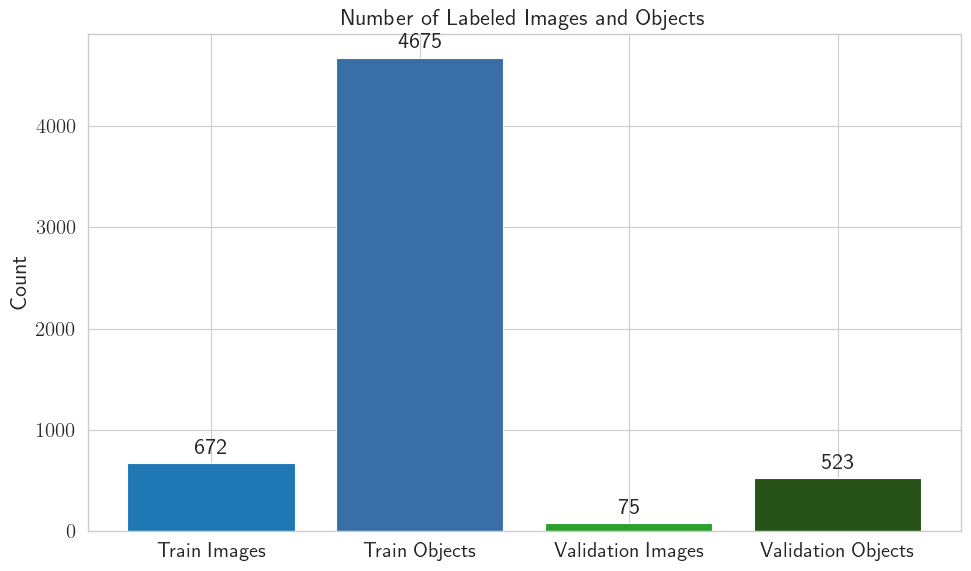
\includegraphics[width=0.7\linewidth]{figures/deal_detection/dataset_count.png}
    \caption{Distribution of labeled leaflet pages and deals in training and validation sets.}
    \label{fig:ddetect_dataset_count}
\end{figure*}

The primary focus is on standard deals, as they are the most common and directly useful for consumers. No publicly available dataset fully aligns with this task as it involves both instance segmentation and deal categorization, specifically in the context of German supermarkets. So, a subset of the collected pages was manually annotated. The result is a dataset of 672 annotated leaflet pages, with 4,675 individual deals in training and 75 pages with 523 deals in the validation set as shown in \figref{fig:ddetect_dataset_count}. In cases where no overlapping elements were present, bounding boxes were used. For overlapping offers, instance segmentation masks were created. Depending on the training requirements, annotations can be converted between bounding boxes and segmentation masks, although segmentation masks provide a more granular representation.

% TODO: Referenz auf untenstehende Figures.

\begin{figure*}[h!]
    \centering
    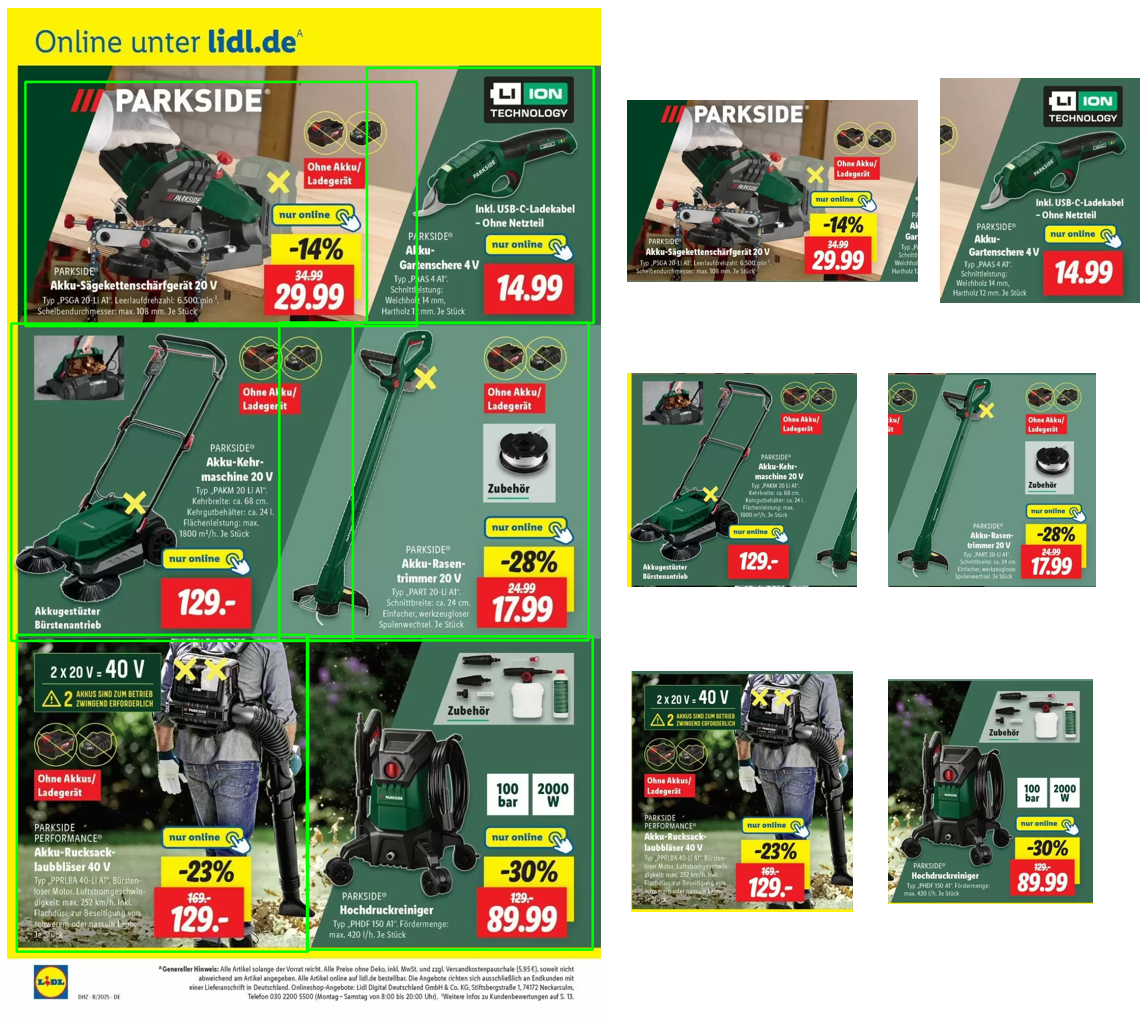
\includegraphics[width=0.6\linewidth]{figures/deal_detection/bbox_page.png}
    \caption{Bounding box detection results on a leaflet page resulting in overlapping bounding boxes.}
    \label{fig:ddetect_bbox_page}
\end{figure*}

\begin{figure*}[h!]
    \centering
    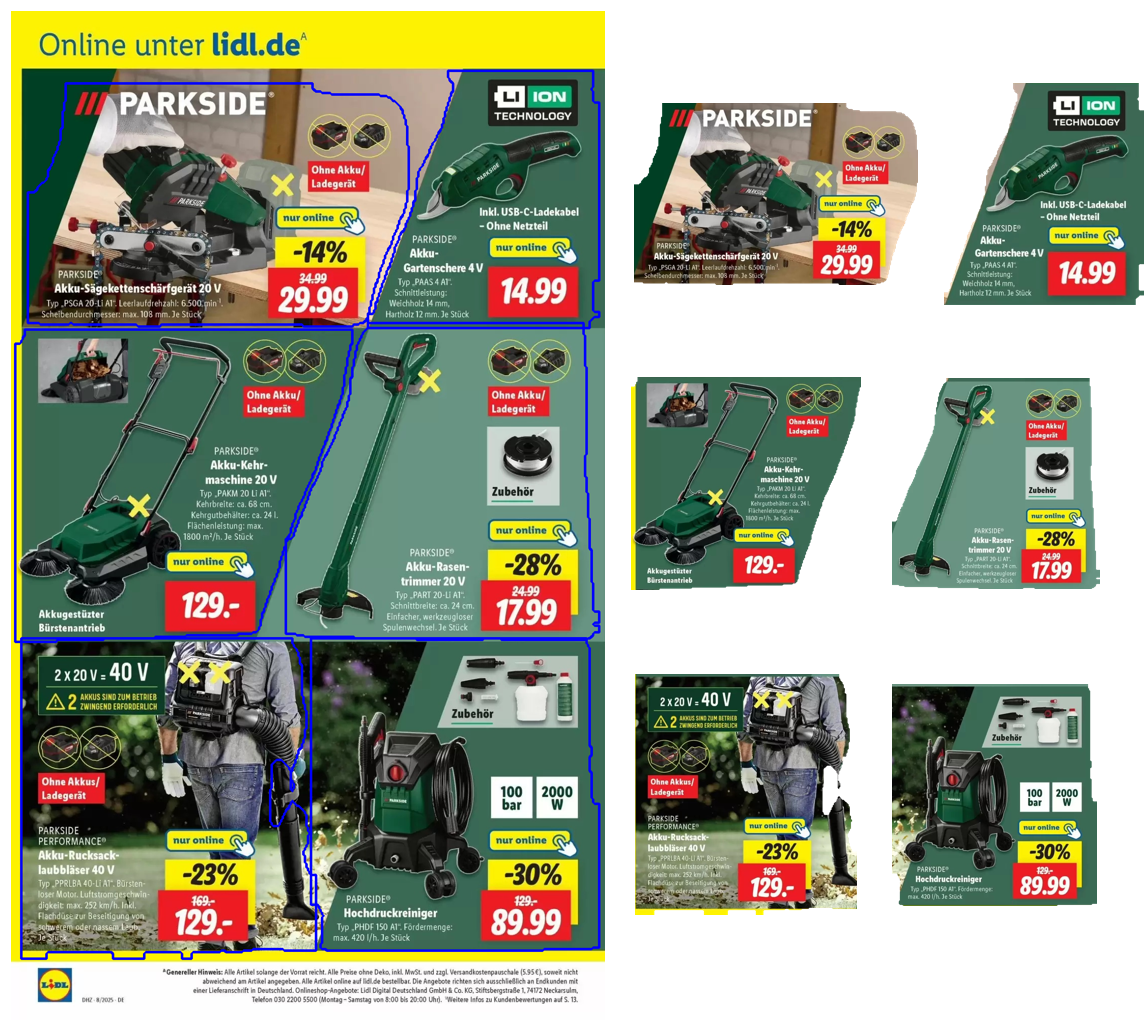
\includegraphics[width=0.6\linewidth]{figures/deal_detection/mask_page.png}
    \caption{Instance segmentation results on a leaflet page showing precise deal separation.}
    \label{fig:ddetect_mask_page}
\end{figure*}

\subsection{Model}
Object detection and segmentation tasks require identifying objects within an image while determining their locations. The simplest form of image analysis, image classification, assigns a single label to an entire image, providing no information about object positions. However, multiple deal detection in supermarket leaflets demands the identification of multiple deals, whose number is unknown beforehand, along with their precise locations to extract them later.

Object detection models can be broadly categorized into multi-stage (multi-shot) detectors and single-stage (single-shot) detectors. Multi-stage detectors, such as the R-CNN family (R-CNN, Fast R-CNN, Faster R-CNN, Mask R-CNN), follow a sequential process. First, they generate a set of region proposals, indicating potential object locations. These proposals are then classified in a second stage. While this method achieves high accuracy, it introduces significant computational overhead. Earlier versions, such as R-CNN, even relied on separate, non-learnable algorithms for proposal generation. Faster R-CNN improved efficiency by integrating the Region Proposal Network (RPN) directly into the model, eliminating the need for external proposal algorithms. However, even this approach remains computationally demanding. In contrast, single-stage detectors, such as YOLO (You Only Look Once), perform detection in a single forward pass, predicting object locations and classifications simultaneously. This significantly reduces inference time, making these models well-suited for real-time applications. YOLO, in particular, has established itself as one of the most widely used architectures due to its speed and competitive accuracy. Given the requirement of processing thousands of leaflet pages efficiently, a single-stage detector was chosen for deal detection, with a particular focus on YOLO-based architectures.

The YOLO model follows a grid-based detection approach, where the input image is divided into an SxS grid. Each grid cell is processed for predicting objects whose centers fall within it. Instead of relying on separate region proposal mechanisms, YOLO processes the image in a single forward pass, directly predicting bounding box coordinates, confidence scores, and class probabilities per grid cell. The bounding boxes are parameterized by their center coordinates, width, and height, while the confidence scores indicate the model’s certainty that a given bounding box contains an object. The class probabilities further specify which category the detected object belongs to. Traditional object detection frameworks like YOLO produce bounding boxes that encapsulate detected objects in rectangular shapes. However, supermarket leaflets contain deals that frequently overlap or feature irregular layouts, making bounding box-based detection less effective. Instance segmentation extends YOLO by incorporating an additional segmentation head that predicts pixel-level masks for each detected object. This approach enables the model to distinguish individual deals more precisely, reducing the risk of grouping multiple offers within a single bounding box. The segmentation mechanism operates by first detecting objects using the standard YOLO pipeline. Once a bounding box is identified, the model refines its prediction by generating a binary mask that determines which pixels within the bounding box belong to the detected object. The segmentation head shares feature representations with the object detection components, ensuring efficient training and inference. This method enhances the model’s ability to isolate individual deals even in cluttered layouts, making it particularly suited for supermarket leaflets where offers frequently overlap or appear with complex backgrounds.

\subsection{Experiments}
Evaluating the performance of instance segmentation models requires an analysis of how well detected objects align with ground-truth annotations. The primary metric used in this assessment is \emph{Mean Average Precision (mAP)}, which quantifies detection accuracy at different levels of overlap between predicted and actual objects. The core component of mAP is Intersection over Union (IoU). IoU is defined as the ratio of the intersection area between the predicted and ground-truth segmentation masks to their union. A higher IoU indicates a better match between the prediction and the actual object, while a lower IoU suggests that the detected region is misaligned or includes excessive background. In the case of bounding boxes, IoU is calculated based on the overlap of rectangular regions, whereas for instance segmentation, it is computed on a pixel level, capturing the true shape of the detected objects. To evaluate model performance, different IoU thresholds are applied. A commonly used metric is mAP@50, which considers a detection correct if the IoU between the predicted and ground-truth mask exceeds 50\%. This threshold provides insight into how well a model identifies objects in general but does not strictly enforce precision in localization. A more comprehensive metric is mAP@50-95, which averages precision across multiple IoU thresholds, ranging from 50\% to 95\% in increments of 5\%. This approach penalizes models that fail to produce accurate segmentations and is particularly useful for assessing how well the model distinguishes closely packed or irregularly shaped deals.

\begin{figure*}[h!]
    \centering
    \begin{tabular}{cc}
    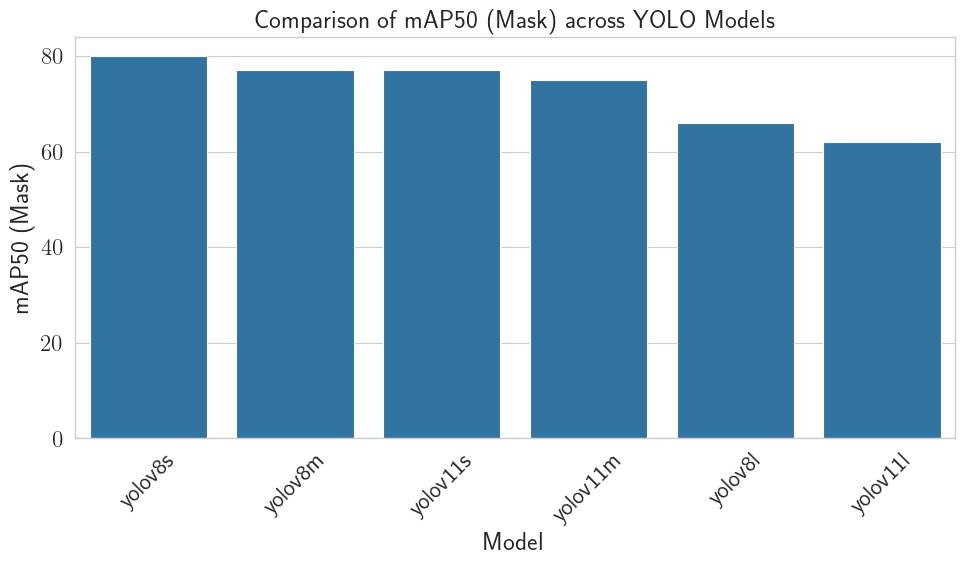
\includegraphics[width=0.5\linewidth]{figures/deal_detection/map50_all_yolo.png} &   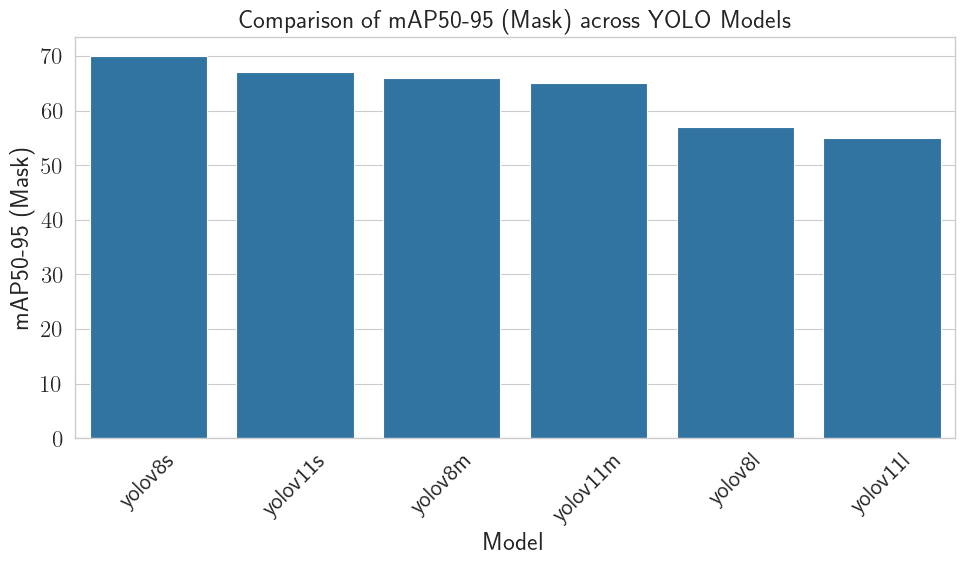
\includegraphics[width=0.5\linewidth]{figures/deal_detection/map50_95_all_yolo.png} \\
    (a) Results for mAP50 & (b) Results for mAP50-95 \\[2pt]
    \end{tabular}
    \caption{Performance comparison of YOLOv8 and YOLOv11 models on the deal detection validation set.}
    \label{fig:all_yolo_results}
\end{figure*}

The first set of experiments focused on comparing different YOLO variants trained on the dataset. Each model was trained for 20 epochs without additional data augmentation. The results, shown in Figure \ref{fig:all_yolo_results} (a), present the mAP50 (mask) scores for YOLOv8 and YOLOv11 in their small, medium, and large configurations. The findings indicate that the smallest version of YOLOv8 achieved the highest validation mAP50, outperforming larger models in this setting. A second analysis, visualized in Figure \ref{fig:all_yolo_results} (b), examines mAP50-95 scores for the same models, reinforcing the observation that a lightweight YOLO model is sufficient for this particular task. The lower performance of larger models suggests that the dataset’s structure, with relatively uniform layouts, does not require highly complex architectures to achieve strong results.

\begin{figure*}[h!]
    \centering
    \begin{tabular}{cc}
    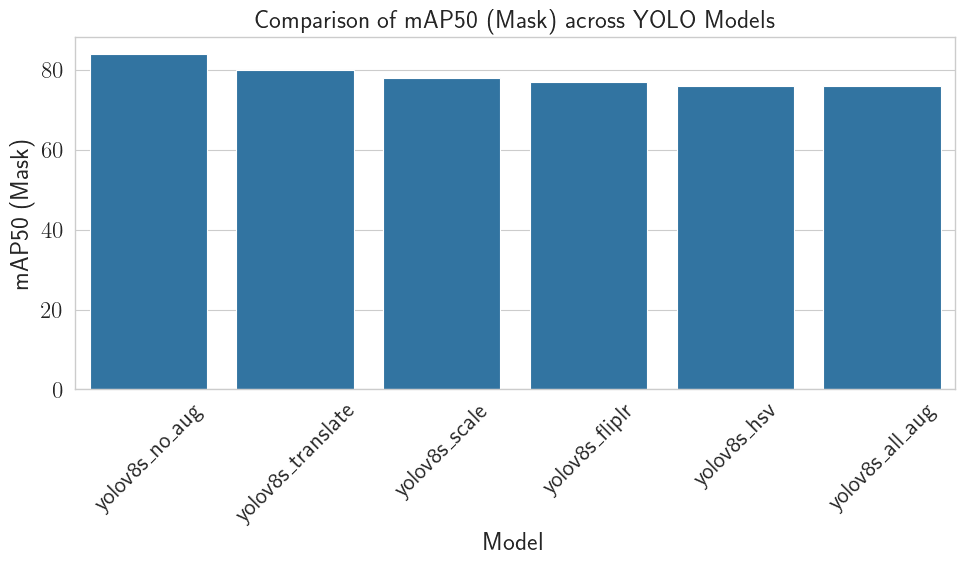
\includegraphics[width=0.5\linewidth]{figures/deal_detection/map50_yolo8.png} &   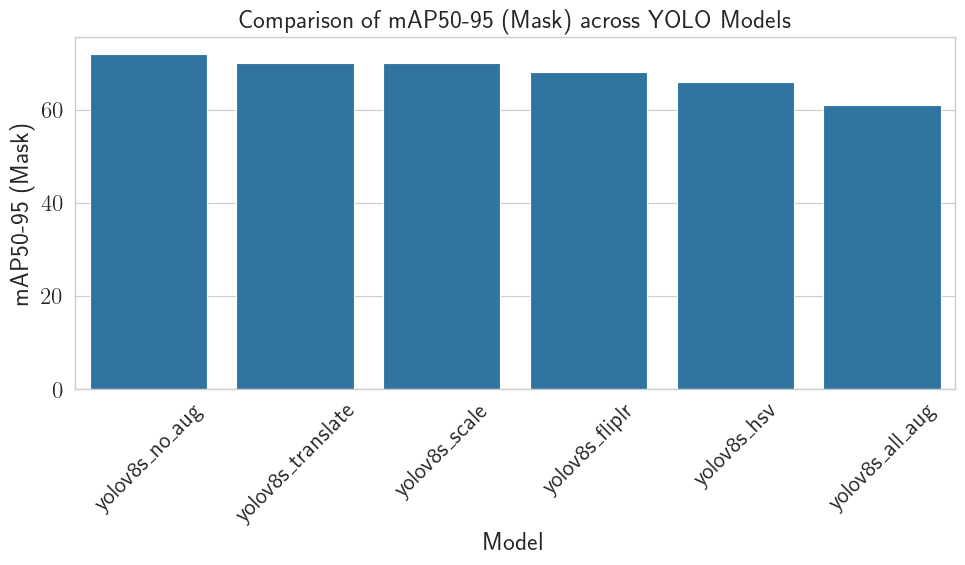
\includegraphics[width=0.5\linewidth]{figures/deal_detection/map50_95_yolo8.png} \\
    (a) Results for mAP50 & (b) Results for mAP50-95 \\[2pt]
    \end{tabular}
    \caption{Performance comparison of YOLOv8s models with and without data augmentation on the deal detection validation set.}
    \label{fig:yolo8_results}
\end{figure*}

Following this baseline evaluation, additional experiments investigated the impact of data augmentation on segmentation performance. Various augmentation strategies were applied, including translation, scaling, horizontal flipping, and color transformations. The goal was to determine whether these transformations improved the model’s ability to generalize across different leaflet layouts. Each augmented model was trained for ten additional epochs, and the results are displayed in Figure \ref{fig:yolo8_results}. While certain augmentation techniques led to slight improvements in segmentation accuracy, particularly for models trained with random translations, the overall best-performing model remained the one trained without any augmentation. This outcome suggests that the dataset already contains sufficient variation to ensure robust generalization without the need for extensive artificial augmentations.

The final model selection was based on the combination of high segmentation accuracy and computational efficiency. Given the results, \emph{YOLOv8s} was chosen as the preferred model, as it consistently outperformed more complex variants while maintaining a lower computational cost. The model’s ability to detect deals with high precision makes it a strong candidate for further applications. And this is particularly important because everything else builds on it.

\section{Information Extraction of Supermarket Deals}
\label{sec:information_extraction}
Subsequently to the detection and separation of supermarket deals, the overarching goal of using these in applications requires the extraction of the various useful information from these deals. 
The task of extracting meaningful and structured information from supermarket deal images is a complex and multi-faceted problem, requiring the integration of various modalities, overcoming challenges posed by noisy data, and leveraging deep learning techniques. This section provides a detailed exploration of methodologies, as well as the theoretical and practical framework needed to perform such extraction.

\subsection{Approaches to Information Extraction}
Formally, the task of information extraction from a deal image can be defined as the identification of specific entities, including the product name, brand, original price, deal price, and unit. We define the following set of output labels:
\begin{equation}
\mathcal{Y} = \{y_{i}\}_{i=1}^{n},
\end{equation}
where $y_{i}$ represents the $i$-th entity in the deal image. In the following, the entities are defined as:
\begin{itemize}
    \item \code{$y_{\text{product\_name}}$}: The name of the product.
    \item \code{$y_{\text{brand}}$}: The brand of the product.
    \item \code{$y_{\text{original\_price}}$}: The original price of the product.
    \item \code{$y_{\text{deal\_price}}$}: The deal price of the product.
    \item \code{$y_{\text{unit}}$}: The unit of the product (e.g., weight, volume).
\end{itemize}

To extract these entities, the target is to learn a function $f(\cdot)$ that maps an input image $I$ to the desired outputs:
\begin{equation}
    f: I \to \mathcal{Y},
\end{equation}
where $ I $ is the deal image, and $ \mathcal{Y} $ represents the extracted entities.

The choice of the function $ f(\cdot) $ is an architectural decision that depends on the specific requirements of the task, the nature of the data, the available resources, and the desired performance metrics. 

Among the various existing architectural approaches to learn $ f(\cdot) $ for information extraction, several methodologies have been developed to address the inherent complexities in supermarket deal images. These methods can be categorized into classical approaches, multi-stage traditional models, hybrid OCR-LLM systems, and end-to-end deep learning frameworks. Each paradigm offers distinct advantages, and their applicability depends on computational resources, dataset characteristics, and performance requirements.

\subsubsection{Traditional and Hybrid Approaches for Supermarket Leaflet Information Extraction}  
Information extraction from supermarket leaflets has traditionally been approached through a pipeline of sequential sub-tasks, each addressed by specialized systems. These methods, while extensively studied and methodologically diverse, are typically divided into three main stages: text detection, text recognition, and key-value pair extraction. Although effective in certain scenarios, these approaches suffer from inherent limitations, including computational overhead, error propagation, and suboptimal performance on edge cases. Recent advancements in LLMs have led to the development of hybrid OCR-LLM architectures, which combine the precision of OCR with the contextual reasoning capabilities of LLMs. Below, we formalize these approaches and discuss their strengths and limitations.

Traditional architectures decompose the problem into independent sub-tasks, each handled by specialized models. While this modularity allows for targeted optimization, it introduces complexity and inefficiencies due to the lack of end-to-end training and error propagation across stages.

The first stage, \emph{text detection}, involves identifying regions in the image $ I \in \mathbb{R}^{H \times W \times 3} $ that contain textual information. This is typically achieved using rule-based systems or neural networks designed for small object detection. The output is a set of $ M $ bounding boxes $ \{b_i\}_{i=1}^{M} $, where each $ b_i = (x_{\text{min}}, y_{\text{min}}, x_{\text{max}}, y_{\text{max}}) $ defines the coordinates of a text region. 

Each detected bounding box $ b_i $ is cropped and processed by a \emph{text recognition} model to convert the visual representation into a textual one. This task is challenging due to decoding errors caused by noisy backgrounds, stylized fonts, and ambiguous characters. Given the set of bounding boxes $ \{b_i\}_{i=1}^{M} $, the goal is to predict the corresponding textual entities $ \{t_i\}_{i=1}^{M} $ as the maximum likelihood sequence.

To use the recognized texts for information extraction, the final stage involves parsing the textual entities into structured outputs. This is typically achieved through rule-based systems or sequence-to-sequence models that generate key-value pairs from the recognized text. The output is a set of structured entities $ \{y_i\}_{i=1}^{N} $, where each $ y_i $ represents one of the desired attributes.

The rise of \emph{large language models }(LLMs) has enabled the development of hybrid OCR-LLM architectures, which combine the strengths of OCR tools with the linguistic and reasoning capabilities of LLMs. These approaches retain the traditional OCR pipeline for converting visual text into machine-readable form but leverage LLMs to enhance robustness through contextual reasoning and structured output generation.

In a hybrid OCR-LLM system, the OCR stage processes the input image $ I $ to produce a set of unstructured text fragments $ T = \{t_i\}_{i=1}^{M} $ with associated spatial coordinates. These fragments are serialized into a prompt and fed into a pretrained LLM, which performs contextual parsing and generates some linguistic output that, in most cases, has to be somewhat postprocessed to extract the desired information.

Hybrid OCR-LLM models offer several advantages over traditional pipelines. By integrating contextual reasoning, they reduce error propagation and improve robustness to noisy or ambiguous inputs. Additionally, the use of pretrained LLMs eliminates the need for task-specific training, simplifying system development. However, these models still rely on the accuracy of the OCR stage, and misrecognitions (e.g., "O" vs. "0") can propagate to the LLM. Furthermore, the computational cost of LLM inference can be prohibitive for large-scale applications.

\subsubsection{End-to-End Models}  
End-to-End (E2E) approaches unify document understanding by learning a direct mapping $ F: I \to \mathcal{D} $ and thus jointly optimize visual feature extraction and semantic parsing. We formalize two dominant paradigms: vision-encoder-decoder architectures and large vision-language models (LVLMs), which share foundational principles but diverge in scale and architectural complexity.

Foundationally, all E2E models decompose into three components: a vision encoder, a representation projection, and a decoder. The vision encoder extracts hierarchical visual features $ \mathbf{Z} = \text{Enc}(I) $, which are then aligned with textual semantics through a representation projection. The decoder generates structured output $ \mathbf{Y} $ autoregressively. \figref{fig:e2e_arch} illustrates the unified architecture.

\begin{figure}[h!]
    \centering
    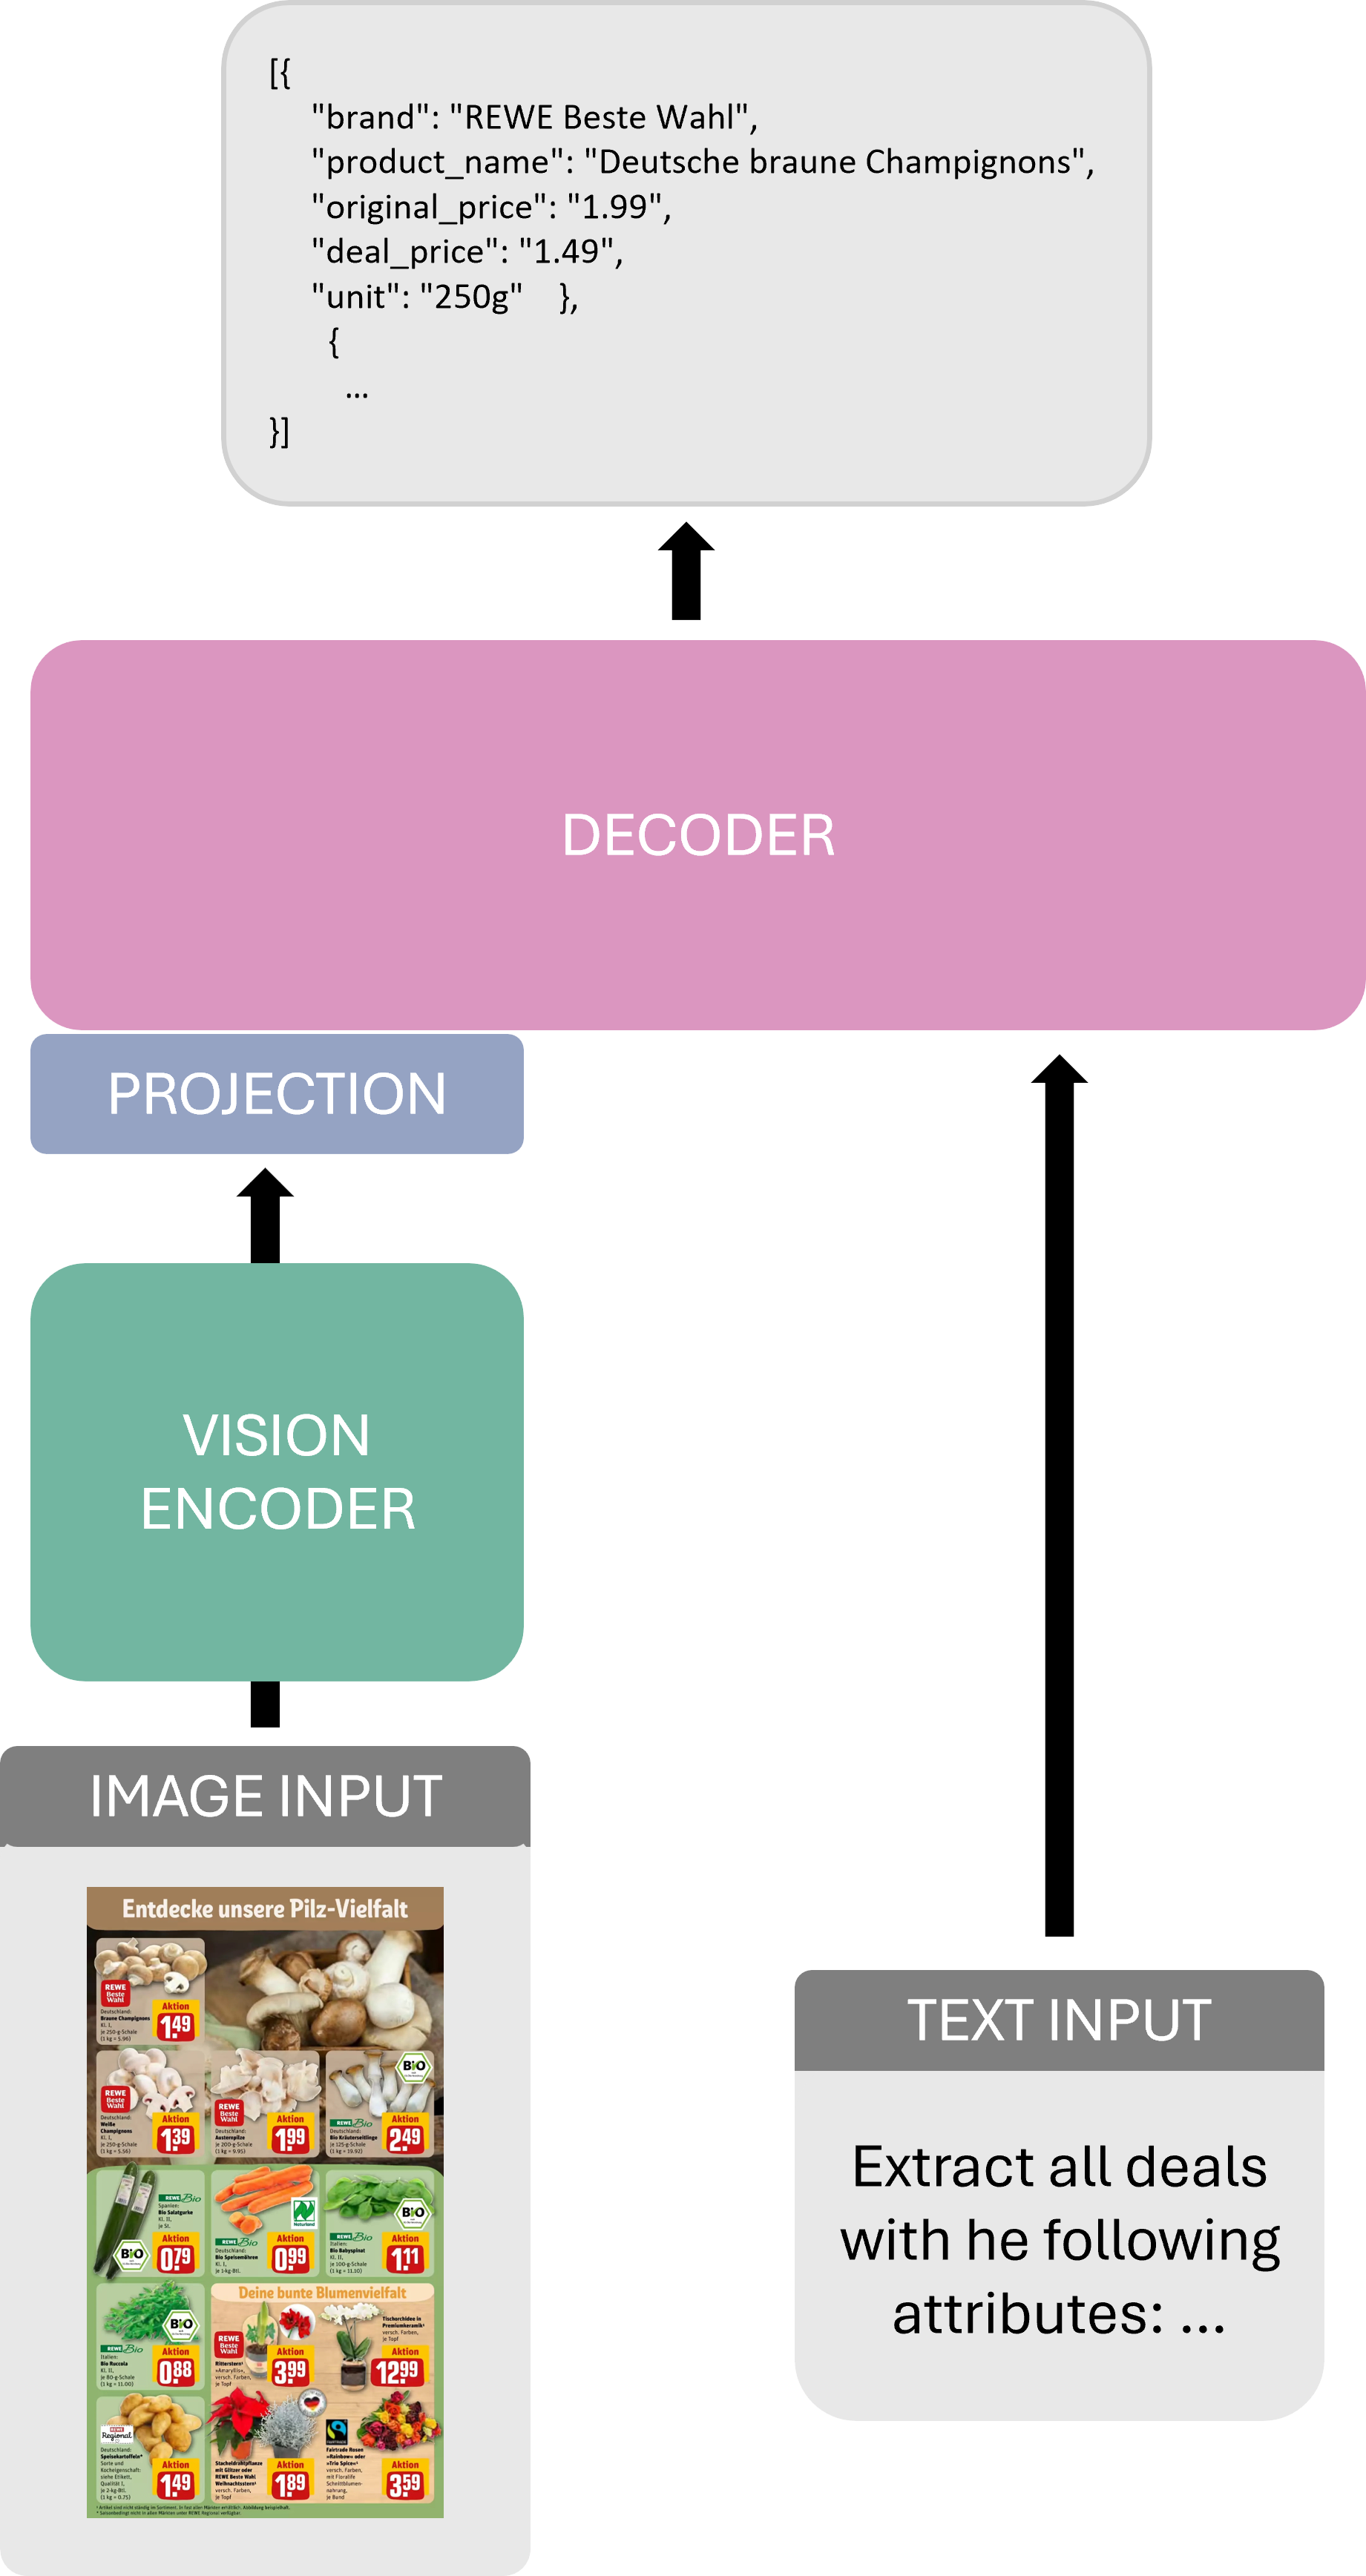
\includegraphics[width=0.5\linewidth]{figures/vlm_arch.png}
    \caption{End-to-End Vision-Encoder-Decoder Architecture.}
    \label{fig:e2e_arch}
\end{figure}

\indent{\textbf{Donut \cite{kim2022}}.} This model employs a compact transformer-based encoder-decoder. Let $ I $ be partitioned into patches, each linearly projected to an encoded input $X$. The used vision encoder $E$ computes an encoded representation mainly through:
\begin{equation}
Z = E(I) = \text{FFN}(\text{MSA}(X) + X) + \text{MSA}(X)
\end{equation}  
where $\text{MSA}$ denotes multi-head self-attention and $\text{FFN}$ a feed-forward network. The hierarchical structure captures local textural patterns as well as global layout cues.  

Subsequently, a transformer decoder generates tokens $ Y = (y_1, \dots, y_T) $ using cross-attention over $ Z $:  
\begin{equation}
P(y_t | y_{<t}, Z) = \text{Softmax}(\text{FFN}(\text{MSA}(Y) + Z)),
\end{equation}  
where $ Y $ is the token sequence and $ Z $ the encoded image features. The model is trained end-to-end with a maximum likelihood objective \cite{vaswani2017}.

\indent{\textbf{Large Vision-Language Models (LVLMs)}.} In the realm of upscaling language models into LLMs, computer vision utilizes this trend to process multimodal data. LVLMs like Llama 3.2 Vision \cite{touvron2023} scale this framework by integrating pretrained vision encoders with LLMs. These architectures utilize \emph{cross-modal projection}, which aligns visual features with the LLM's embedding space, and \emph{multimodal decoding}, which attends to both visual tokens and textual prompts. The LVLM's strength lies in zero-shot reasoning and leveraging pretrained knowledge for structured output generation.

While smaller models like Donut offer efficiency and direct output generation, LVLMs provide zero-shot reasoning and open-world capabilities at increased computational cost.

\subsection{Dataset Creation}

\begin{table}[h!]
    \centering
    \caption{Leaflet-IE Dataset with a sum of 372 annotated deals.}
    \label{tab:ie_dataset}
    \begin{tabular}{lc}
    \toprule
    Entity           & Sample Size \\
    \midrule
    \code{brand}            & 357  \\
    \code{product\_name}    & 370  \\
    \code{original\_price}  & 286  \\
    \code{deal\_price}      & 372  \\
    \code{unit}           & 369  \\
    \bottomrule
    \end{tabular}
\end{table}

Since the availability of German supermarket leaflet data is literally not findable, a custom dataset was created by manually annotating a collection of supermarket deal images. The dataset includes images from the most common supermarket chains, each with unique layout, fonts, and colors to, in general, ensure the highest diversity and robustness possible. Each image is annotated with a corresponding label file that includes the desired entities as well as the image identificator. The dataset is split into a training (\~{} 80\%) 
and a validation set (\~{} 20\%) for each model to be trained and evaluated on. \tabref{tab:ie_dataset} provides an overview of the dataset with the sample size for each entity and \figref{fig:ie_dataset_samples} shows some sample images with their annotations.

Even though the Leaflet-IE dataset is relatively small, the reader will be able to see that the dataset is sufficient to evaluate the performance of different IE appraoches as well as to train an competitive end-to-end model. However, as the reader may notice, the dataset is solely focused on single product deals at this point and explicitly does not include
% TODO: Missing Text (ILYI)

\begin{figure*}[h!]
\centering
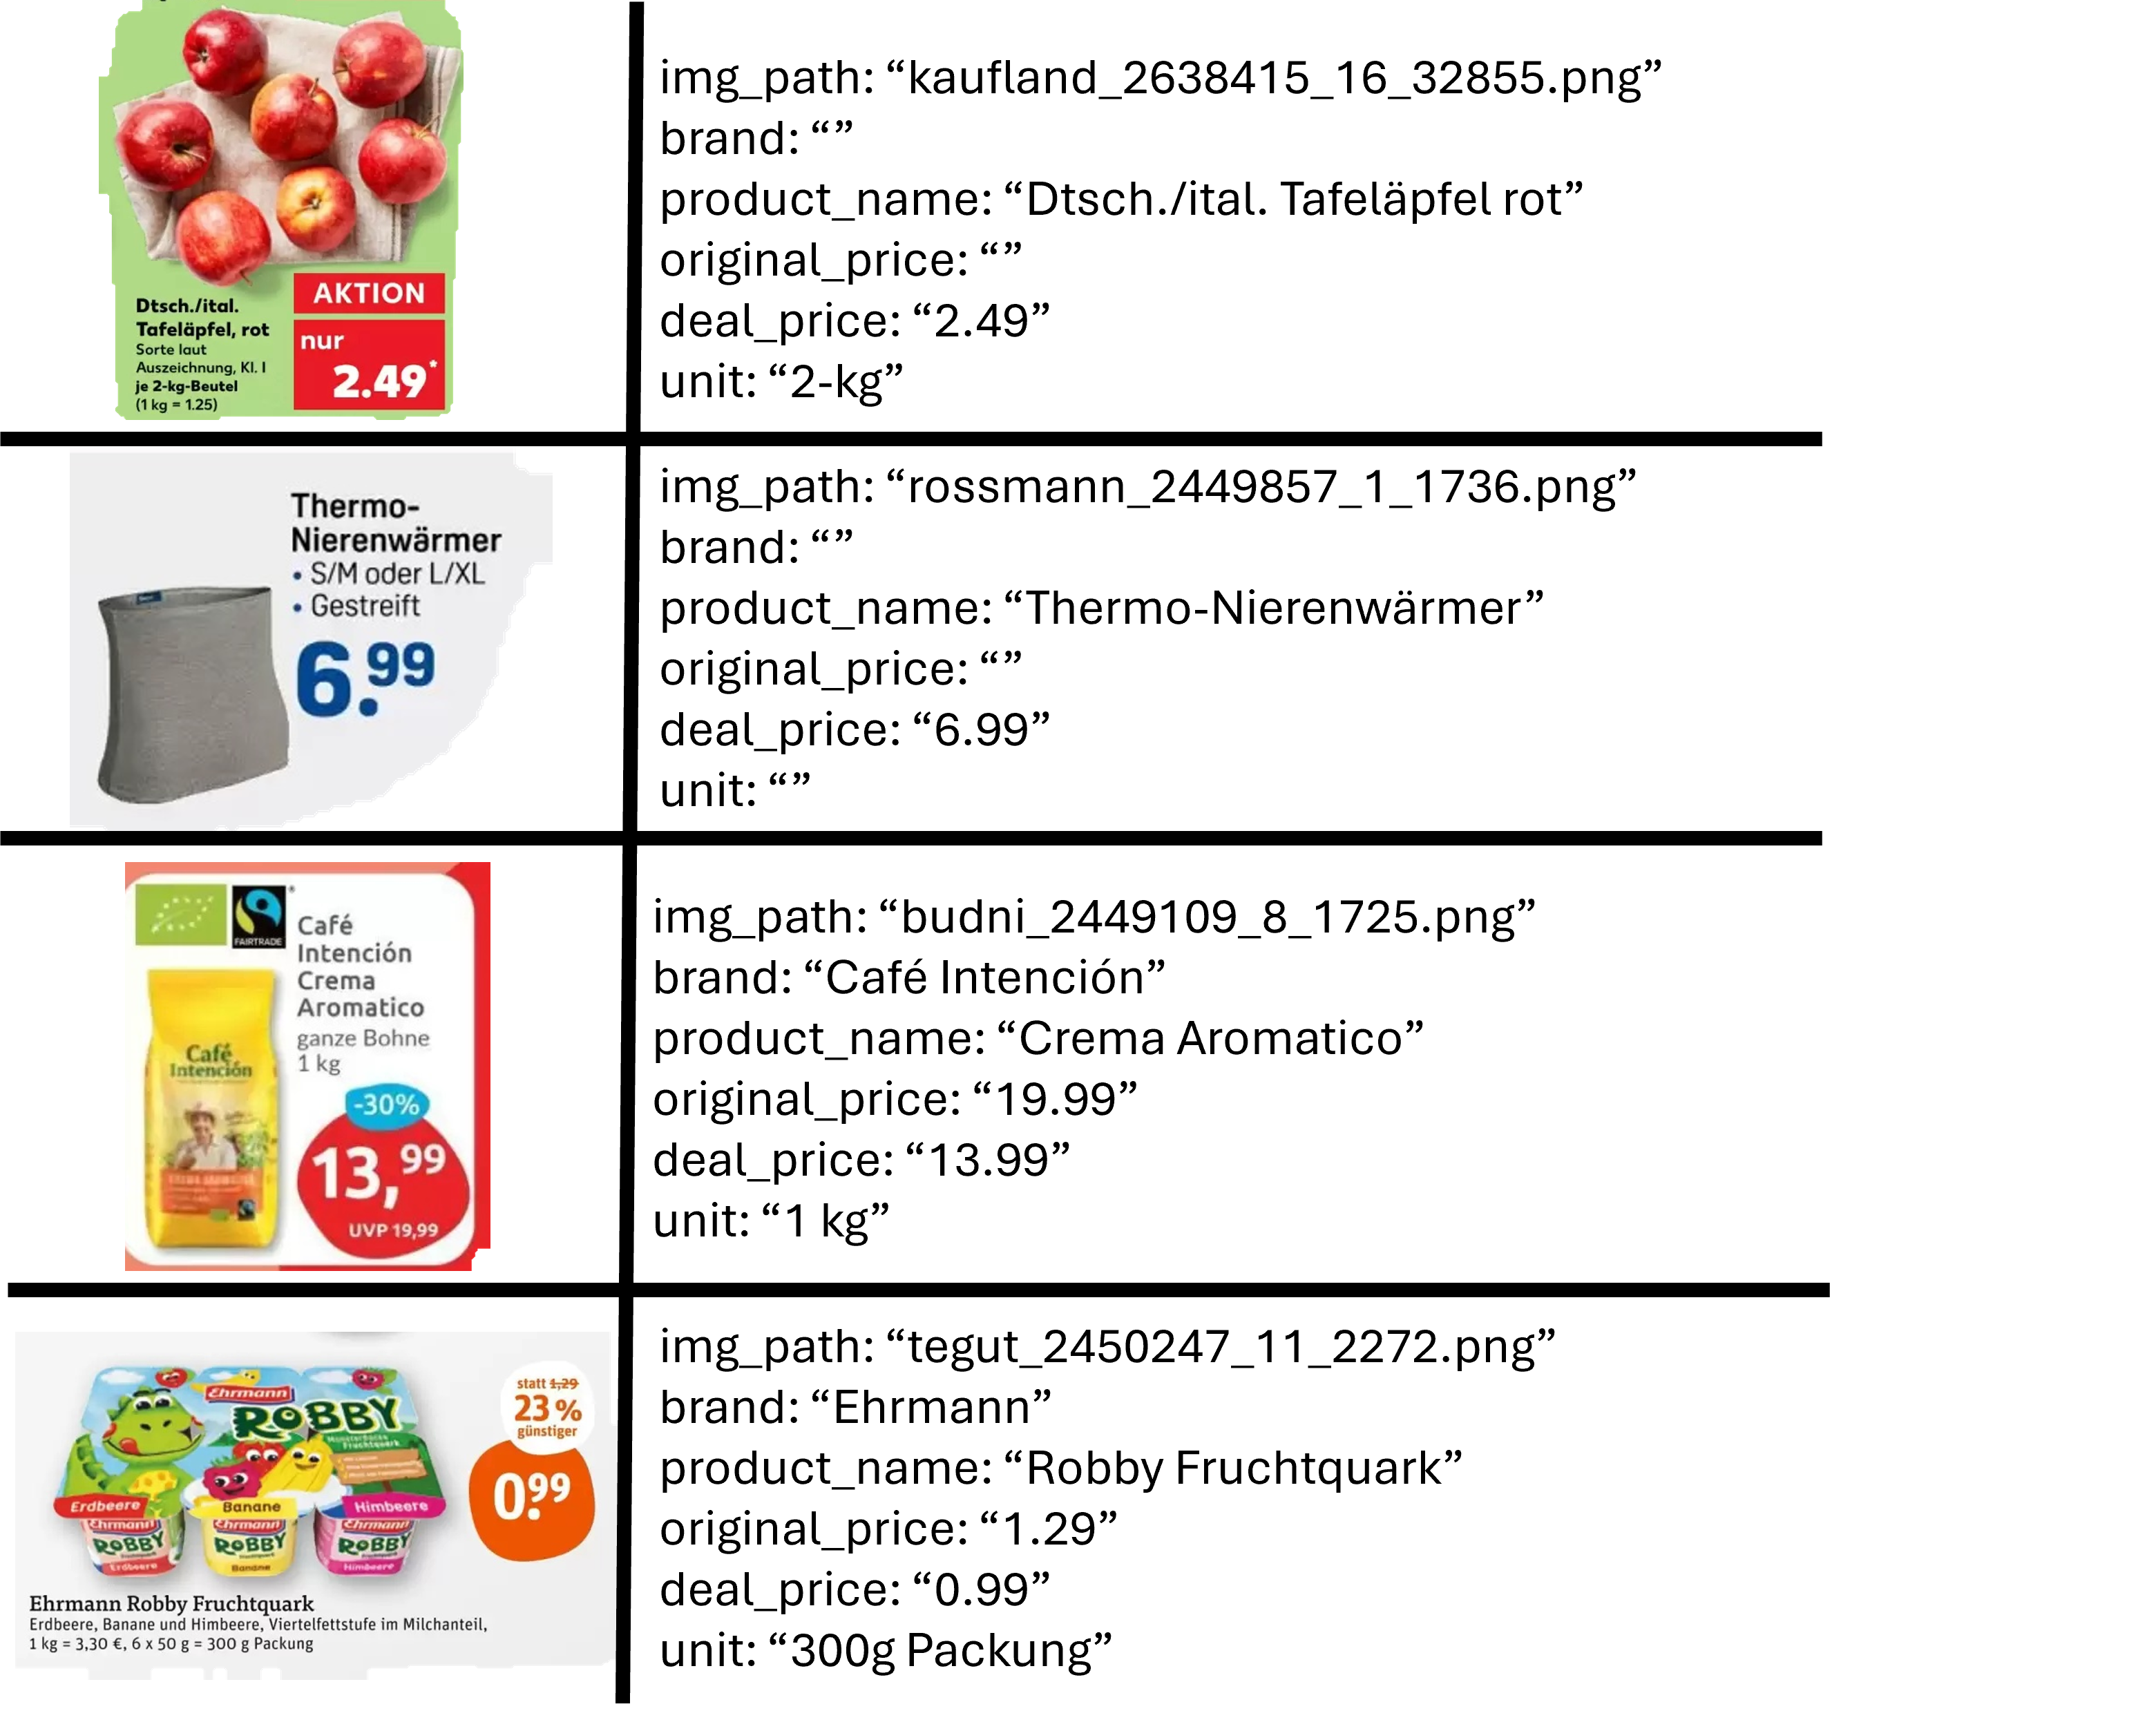
\includegraphics[width=0.5\linewidth]{figures/ie_samples.png}
\caption{Sample images with annotations from the custom dataset.}
\label{fig:ie_dataset_samples}
\end{figure*}

\subsection{Experiments}

% TODO: Remove cause of ambiguity? (ILYI)
% The experiments aim to identify the most effective methodology for extracting structured information from supermarket leaflets by evaluating three candidate approaches: (1) Hybrid OCR + LLM pipelines, (2) end-to-end Vision-Encoder-Decoder models, and (3) LVLMs. The evaluation is structured into four sequential phases to systematically assess performance and scalability.

First, Plain Deal OCR Performance establishes a baseline by measuring the accuracy of standalone OCR systems in extracting textual content from leaflets, highlighting challenges such as font variability and noisy backgrounds. Second, OCR + LLM Performance evaluates the combined pipeline, where OCR outputs are processed by large language models to resolve ambiguities and extract structured information. Third, Donut Fine-Tuning Performance assesses the Vision-Encoder-Decoder model's effectiveness after fine-tuning on leaflet-specific data, focusing on its ability to handle multimodal inputs without intermediate OCR steps. Finally, the MAIN experiment conducts a comprehensive comparison of Hybrid OCR+LLM, Donut, and LVLM approaches, analyzing their accuracy, robustness, and computational efficiency in real-world leaflet data scenarios.


\subsubsection{Implementation Details}
The experiments were conducted on two distinct computational workstations - station 1 equipped with an NVIDIA RTX 4080 GPU and station 2 with an NVIDIA GTX 1080 GPU. Therefore, the experiments could be conducted in parallel, ensuring efficient model training and evaluation.

The software stack includegraphics Python with PyTorch\footnote{\href{https://pytorch.org/}{https://pytorch.org/}} as the primary deep learning framework, HuggingFace Transformers \footnote{\href{https://huggingface.co/transformers/}{https://huggingface.co/transformers/}}
for leveraging pre-trained models, ollama \footnote{\href{https://ollama.com/}{https://ollama.com/}}
and lmstudio \footnote{\href{https://lmstudio.ai/}{https://lmstudio.ai/}} for LVLMs, and OpenCV \footnote{\href{https://opencv.org/}{https://opencv.org/}} for image preprocessing and data augmentation, as well as various other libraries for data pre-and post-processing, visualization, data management and monitoring \footnote{The codebase is available at \href{https://github.com/ilyii/leaflets}{https://github.com/ilyii/leaflets}}.
% TODO: Remove this section or move it to the appendix or introduction because it is also relevant for deal detection chapter? (ILYI)


% SUB-STUDIES
\subsubsection{Plain Deal OCR Performance}
The aim of this experiment is to evaluate the performance of various OCR models in extracting text from supermarket leaflets. The evaluation focuses on the accuracies of the extracted entities from \tabref{tab:ie_dataset} and the impact of different normalization levels on the recognition performance. The results provide insights into the robustness and accuracy of different OCR models in handling the complexities of supermarket leaflet data.

The most commonly used OCR models include:
\begin{itemize}
    \item Tesseract \footnote{\href{https://github.com/tesseract-ocr/tesseract}{https://github.com/tesseract-ocr/tesseract}},
    \item EasyOCR \footnote{\href{https://github.com/JaidedAI/EasyOCR}{https://github.com/JaidedAI/EasyOCR}},
    \item PaddleOCR \footnote{\href{https://github.com/PaddlePaddle/PaddleOCR}{https://github.com/PaddlePaddle/PaddleOCR}},
    \item DocTR \footnote{\href{https://github.com/mindee/doctr}{https://github.com/mindee/doctr}}.
\end{itemize}
These models have been trained on a variety of datasets and are known for their robustness and accuracy in text extraction. Since it is likely that none of the OCR models have seen this data before, all 372 samples of the Leaflet-IE dataset were used for evaluation. While OCR alone is not capable of generating key-value mappings, the evaluation used a different set of metrics:

\begin{itemize}
    \item \textbf{Accuracy}: Measures whether the expected value is present in the OCR output.
    \item \textbf{N-gram Accuracy}: Determines if an n-gram substring of the expected value exists in the OCR output, computed for $n \in \left[\frac{|v|}{2}, |v| - 1\right]$, where $|v|$ represents the string length of the ground truth entity value.
\end{itemize}

Given that language-specific OCR errors are common, the evaluation was conducted at different levels of normalization to improve comparability. The text normalization included the following layers:
\begin{itemize}
    \item \textbf{Level 1:} Text stripping and string conversion.
    \item \textbf{Level 2:} Lowercasing and basic replacements.
    \item \textbf{Level 3:} Use-case specific replacements.
    \item \textbf{Level 4:} Punctuation and whitespace removal.
\end{itemize}
Each level includes the normalization steps of the previous levels. Therefore, the normalization procedure can be thought of as a gradual alignment of the OCR output to the ground truth to investigate the OCR model's robustness to different normalization levels. A detailed description of the normalization procedure can be found in \secref{app:ocr_normalization}.

\indent{\textbf{Results}.} Figure \ref{fig:eval_ocr_accuracies} presents a comparative analysis of various OCR models and normalization levels based on per-entity accuracy. The results highlight several key trends regarding the recognition performance of different entities.

\begin{figure*}
    \begin{tabular}{cc}
      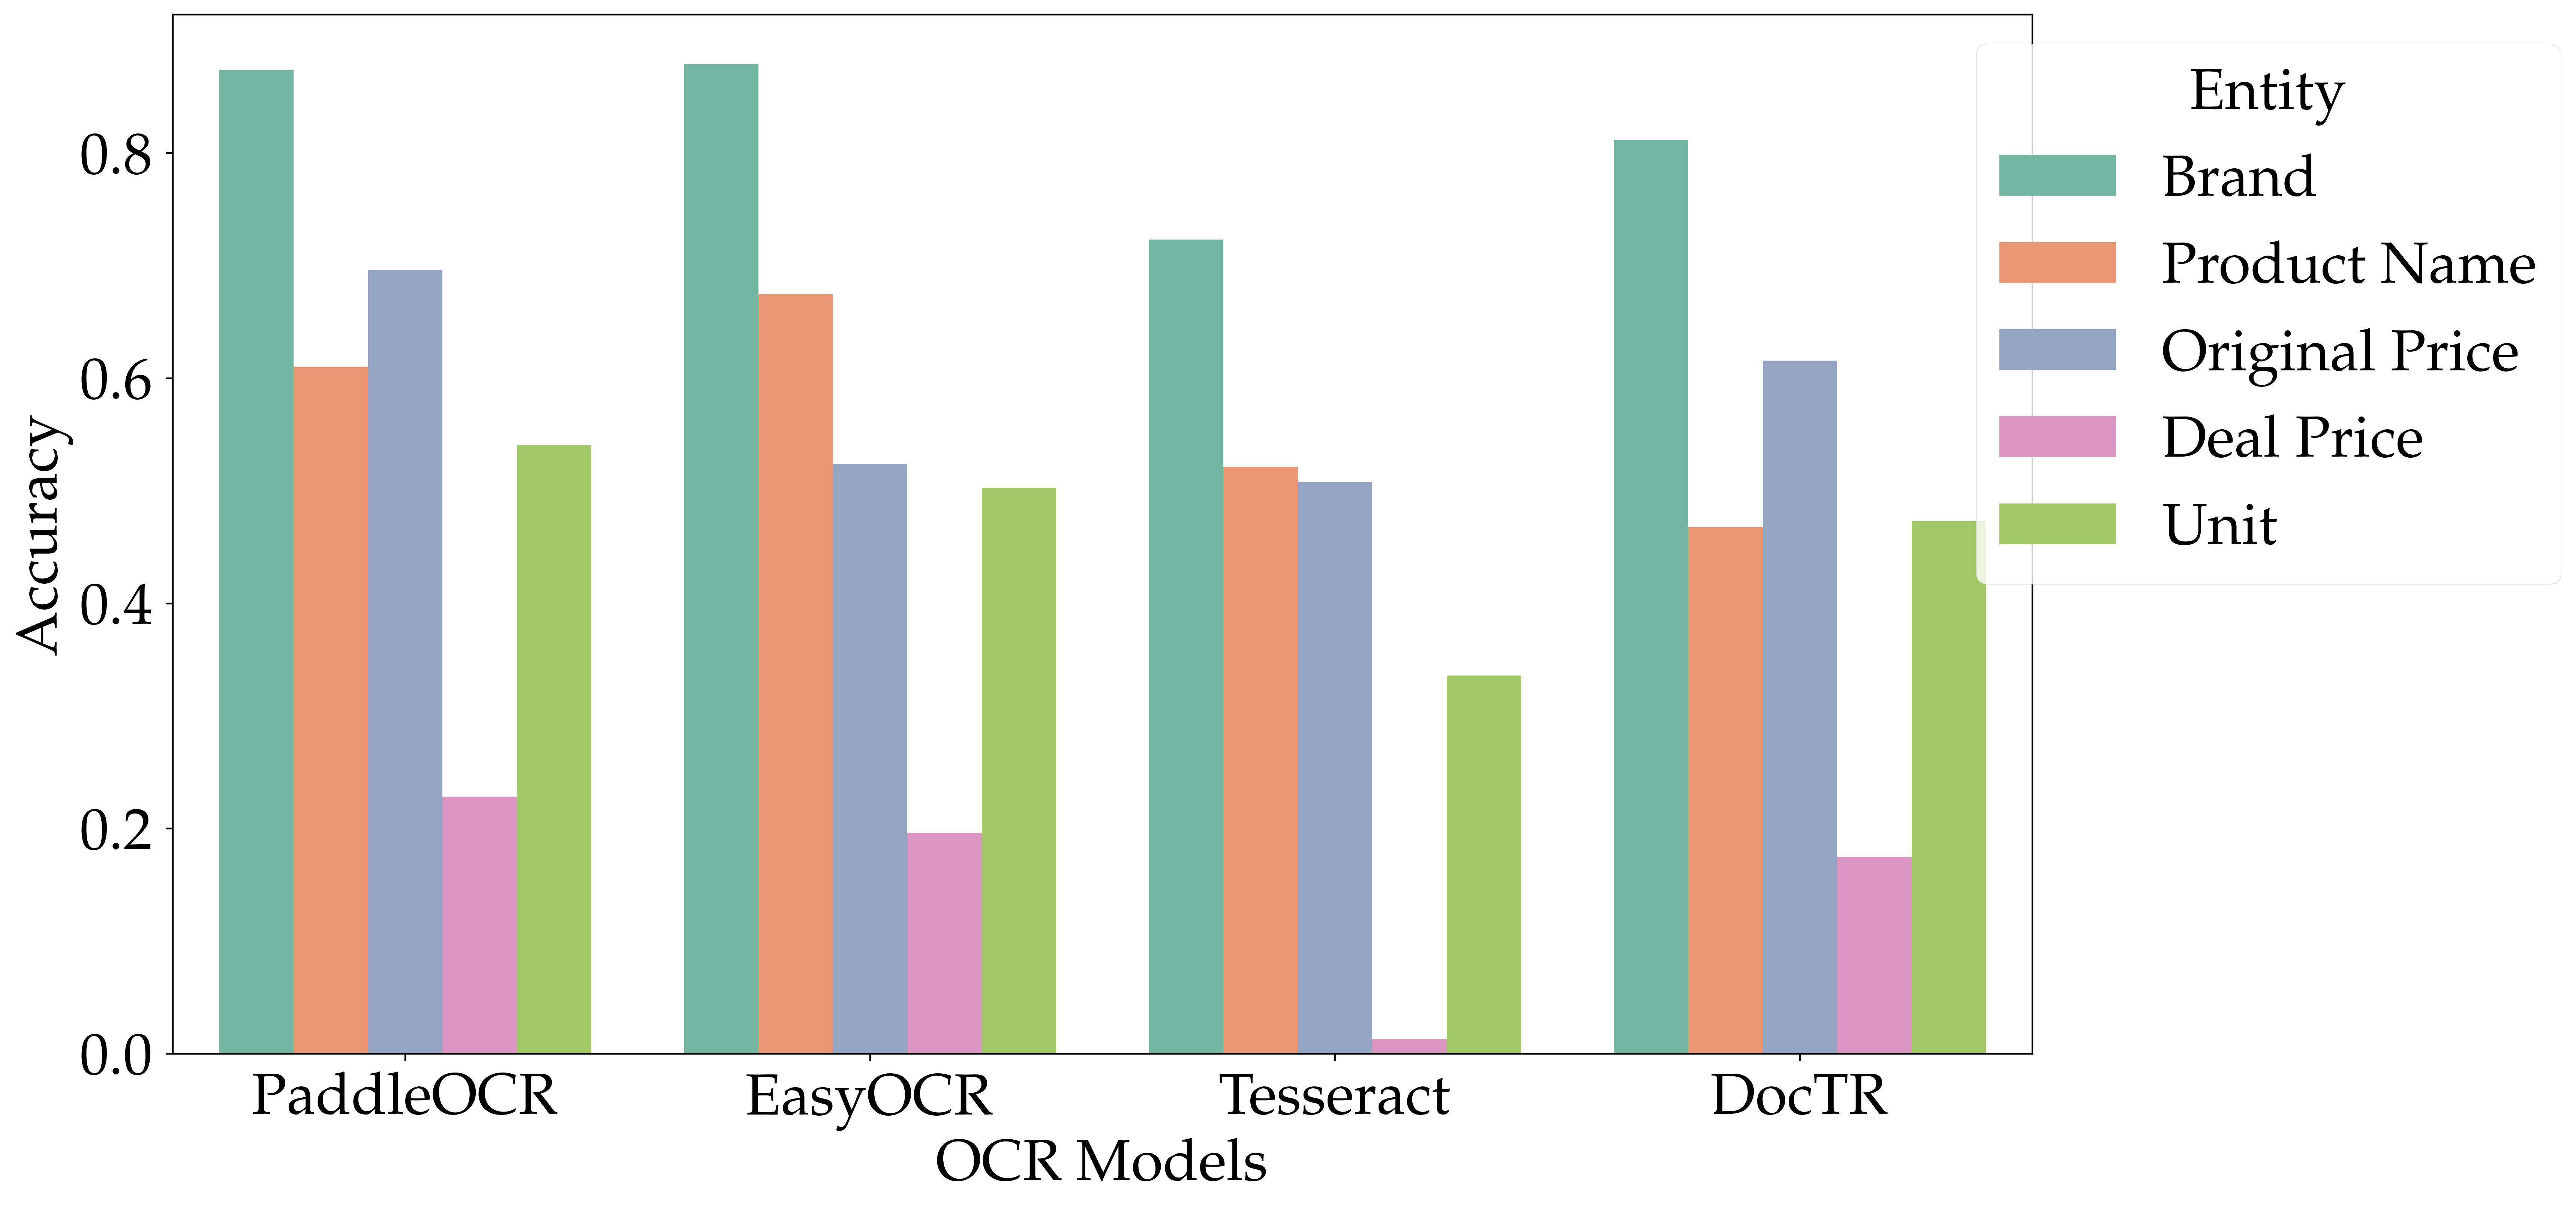
\includegraphics[width=0.5\linewidth]{figures/accuracy_level_1.png} &   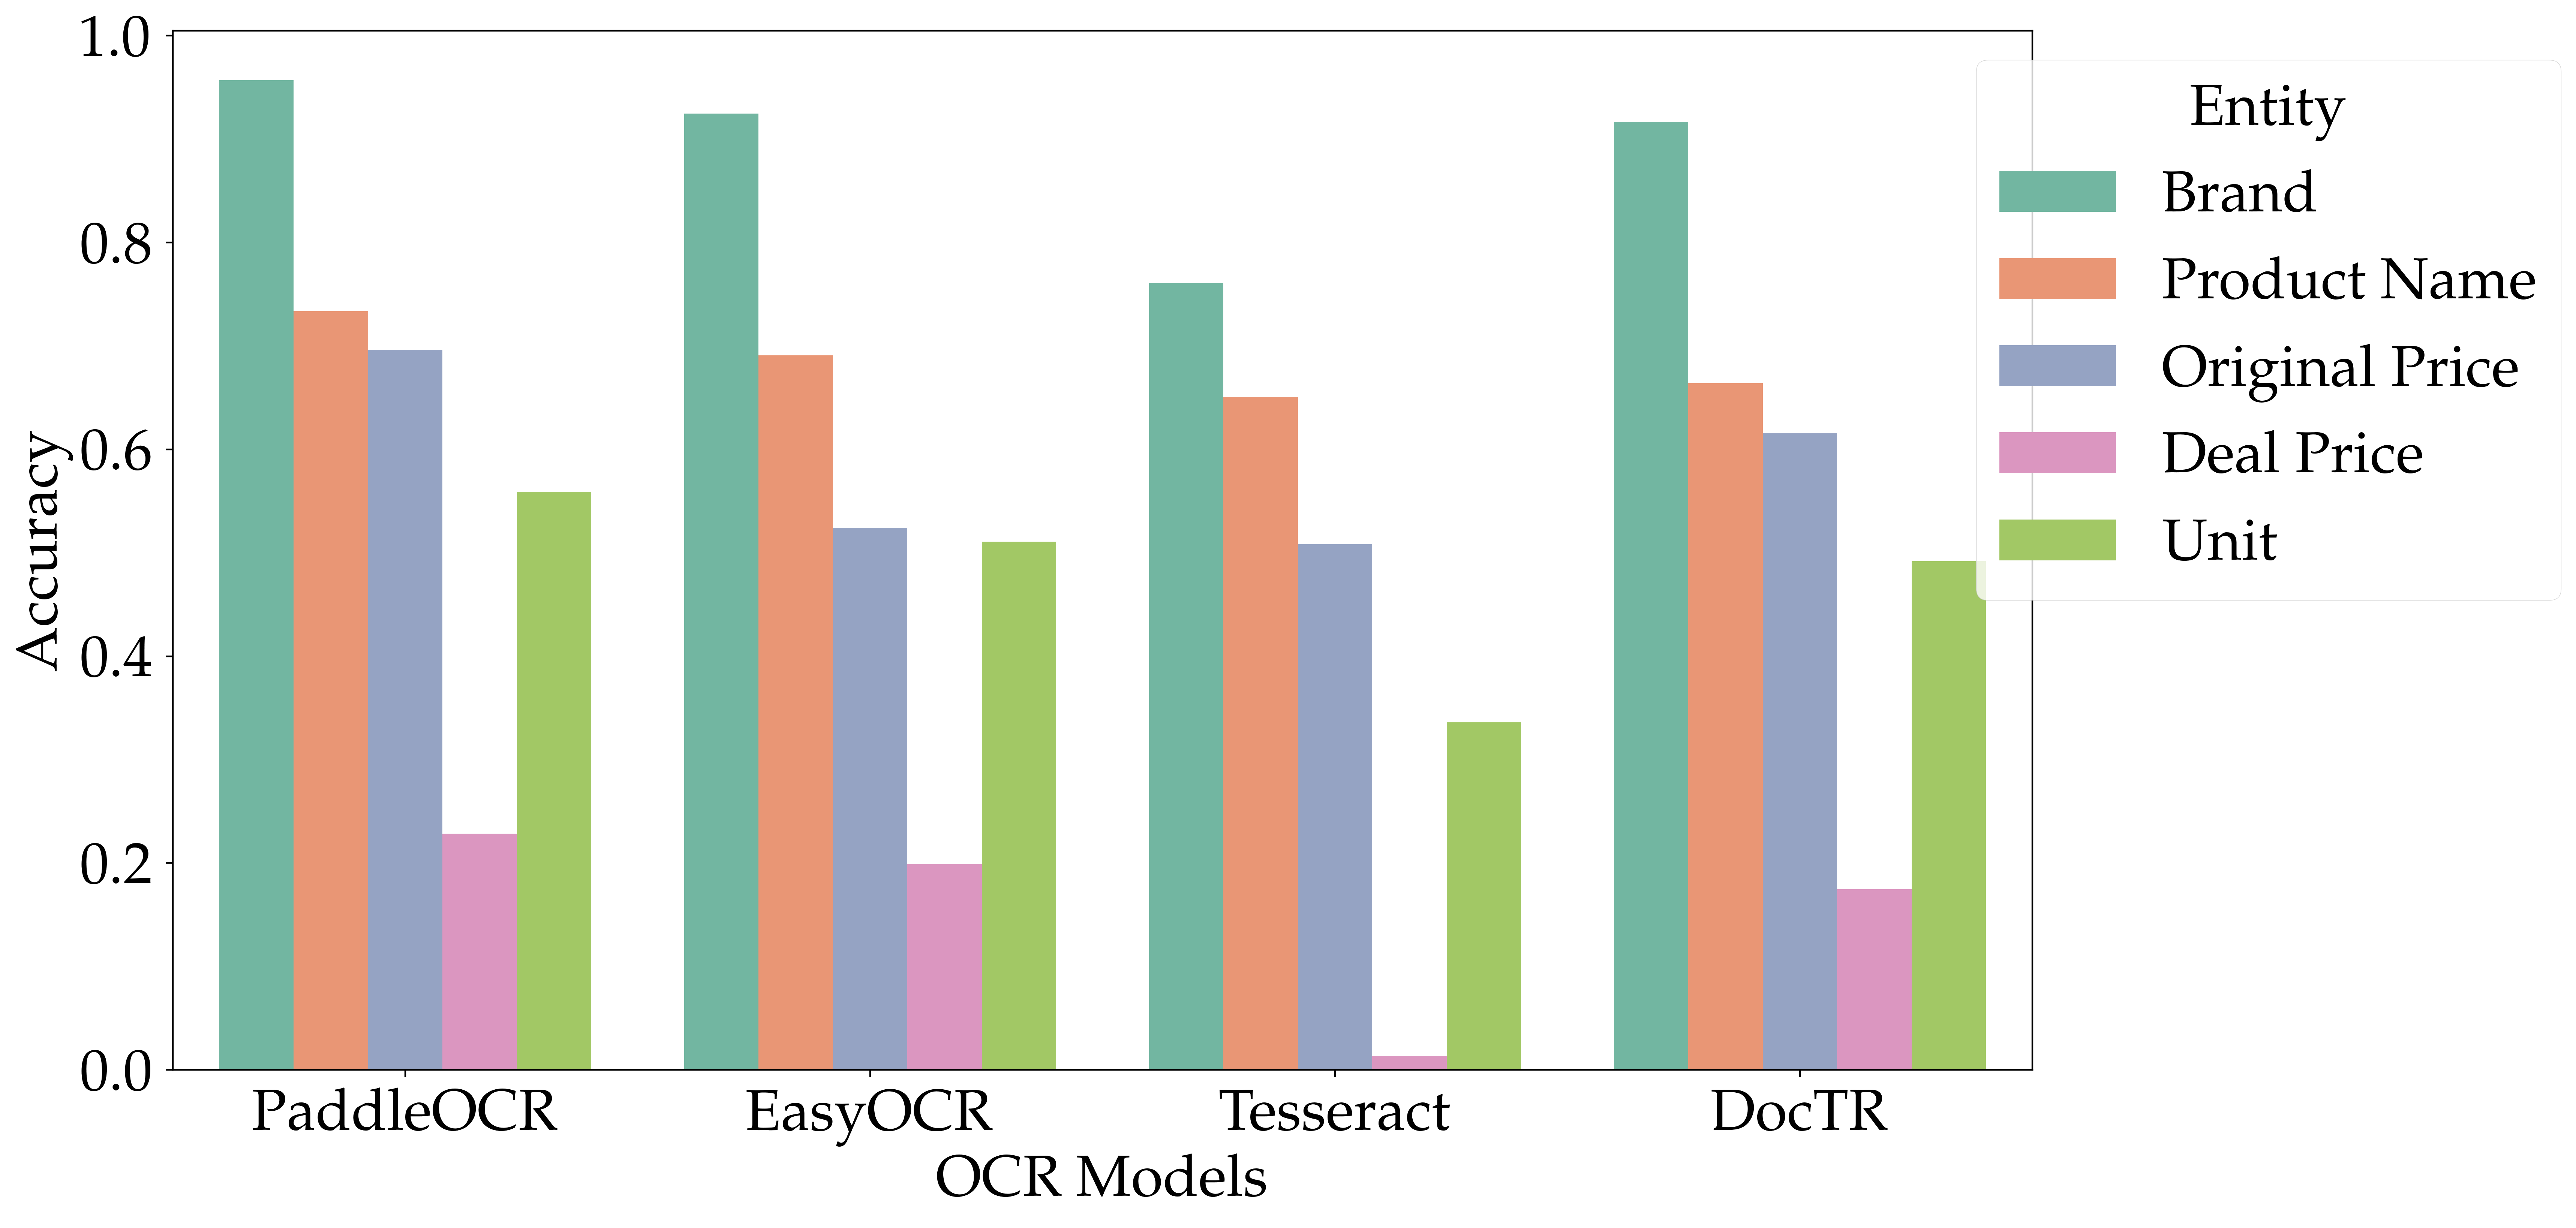
\includegraphics[width=0.5\linewidth]{figures/accuracy_level_2.png} \\
    (a) Level 1 & (b) Level 2 \\[6pt]
     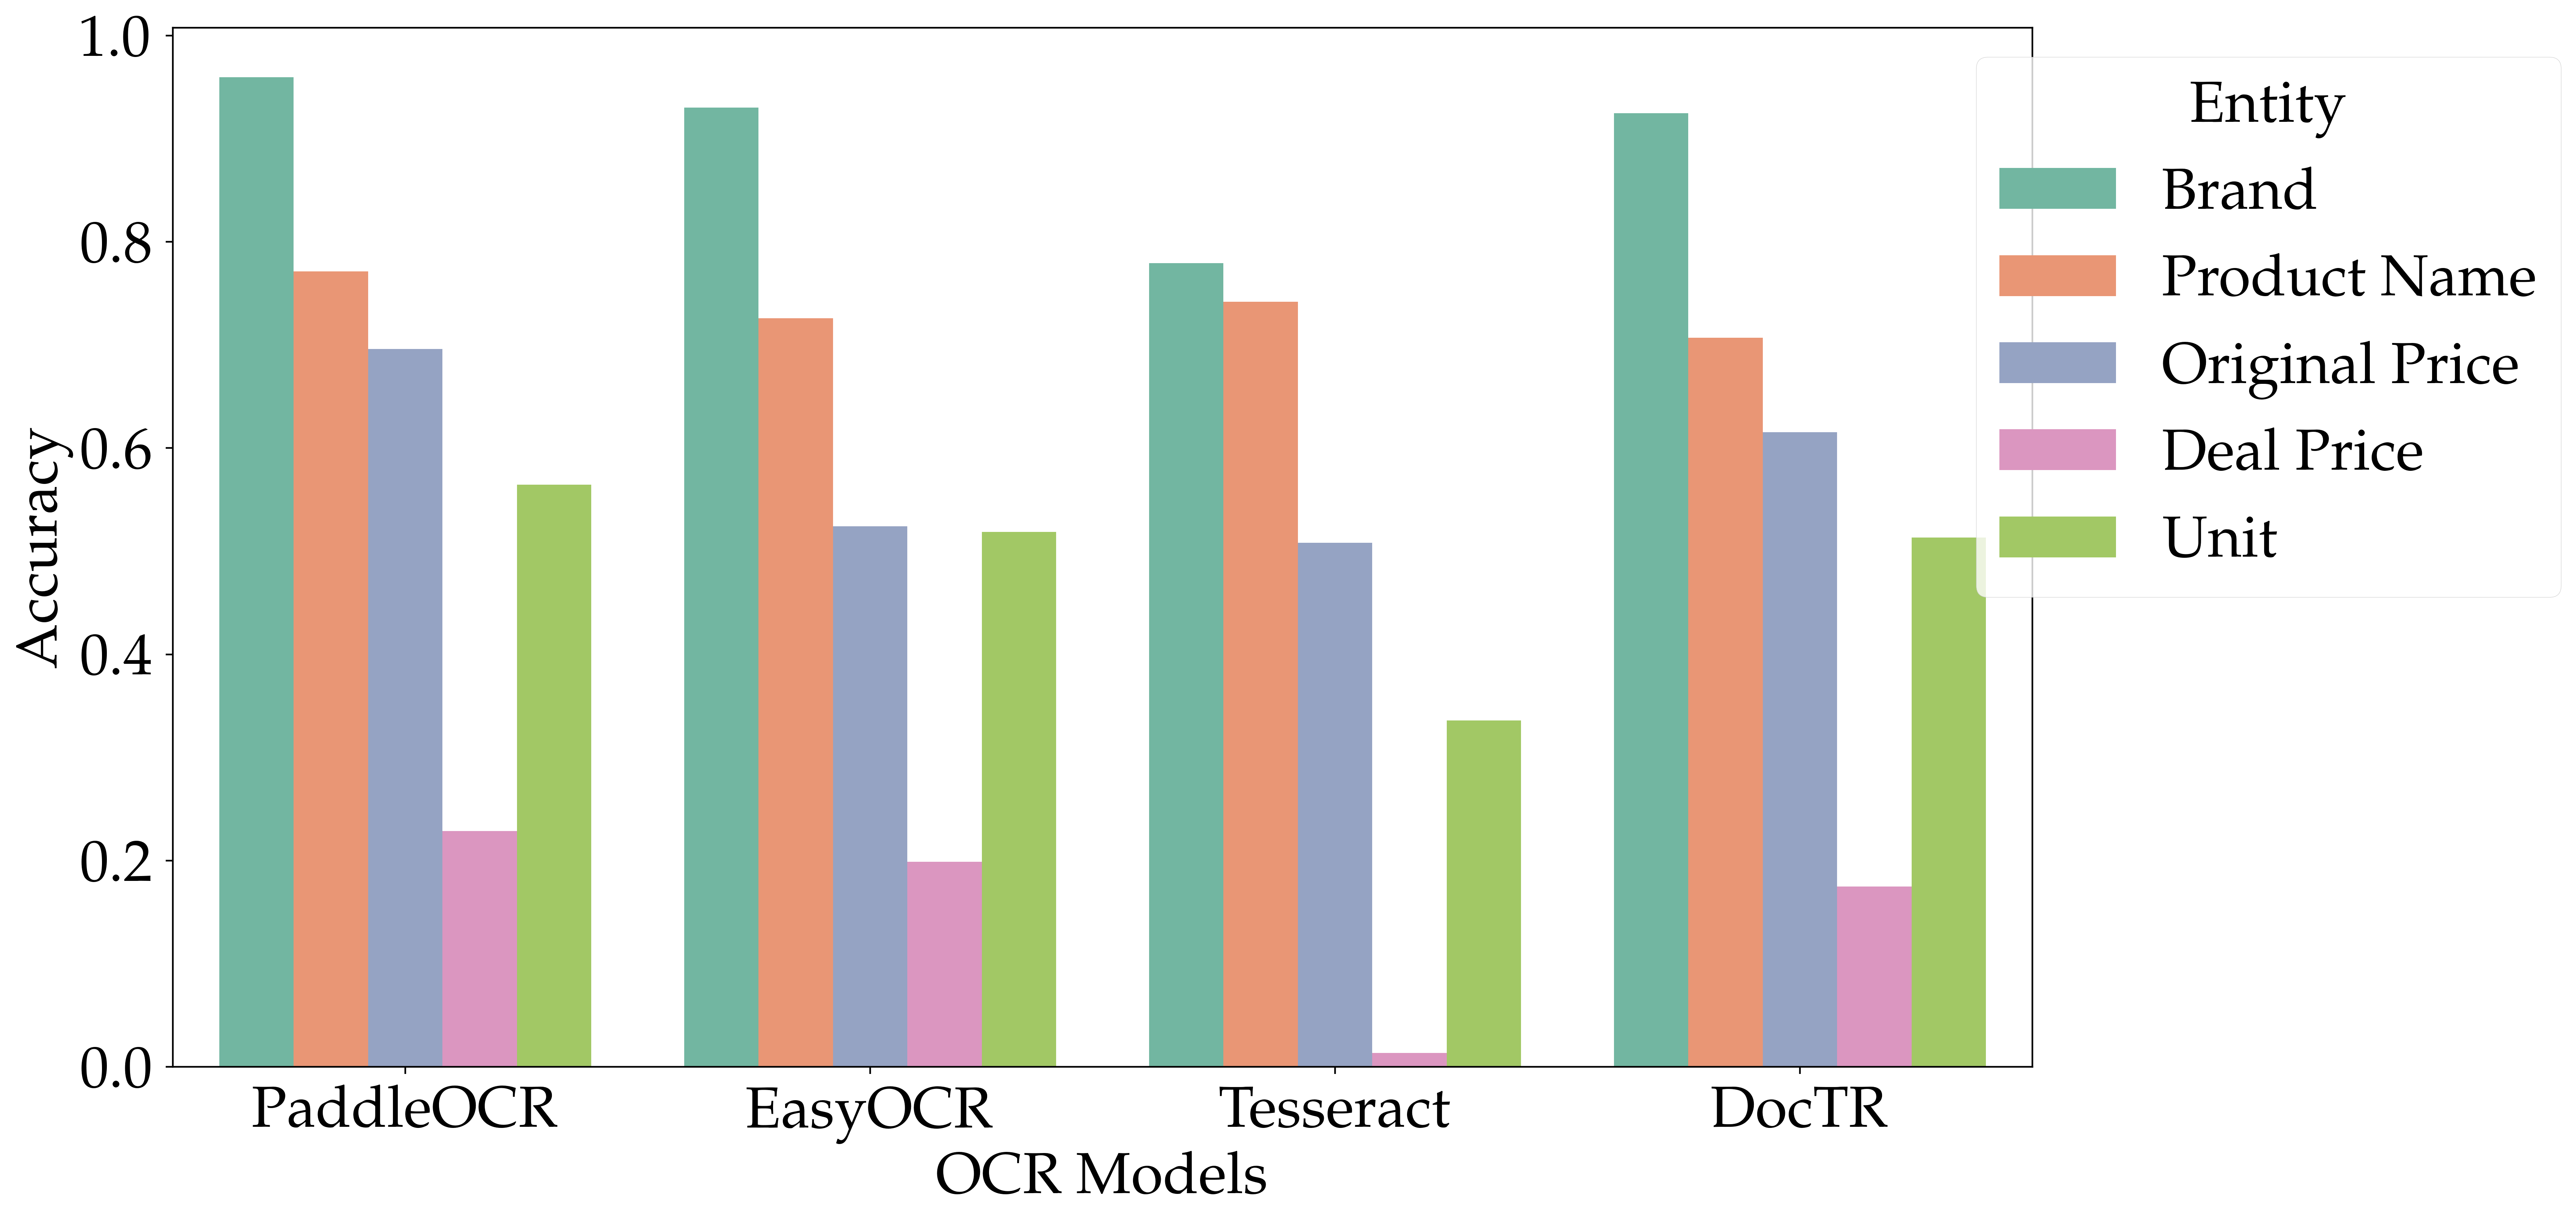
\includegraphics[width=0.5\linewidth]{figures/accuracy_level_3.png} &   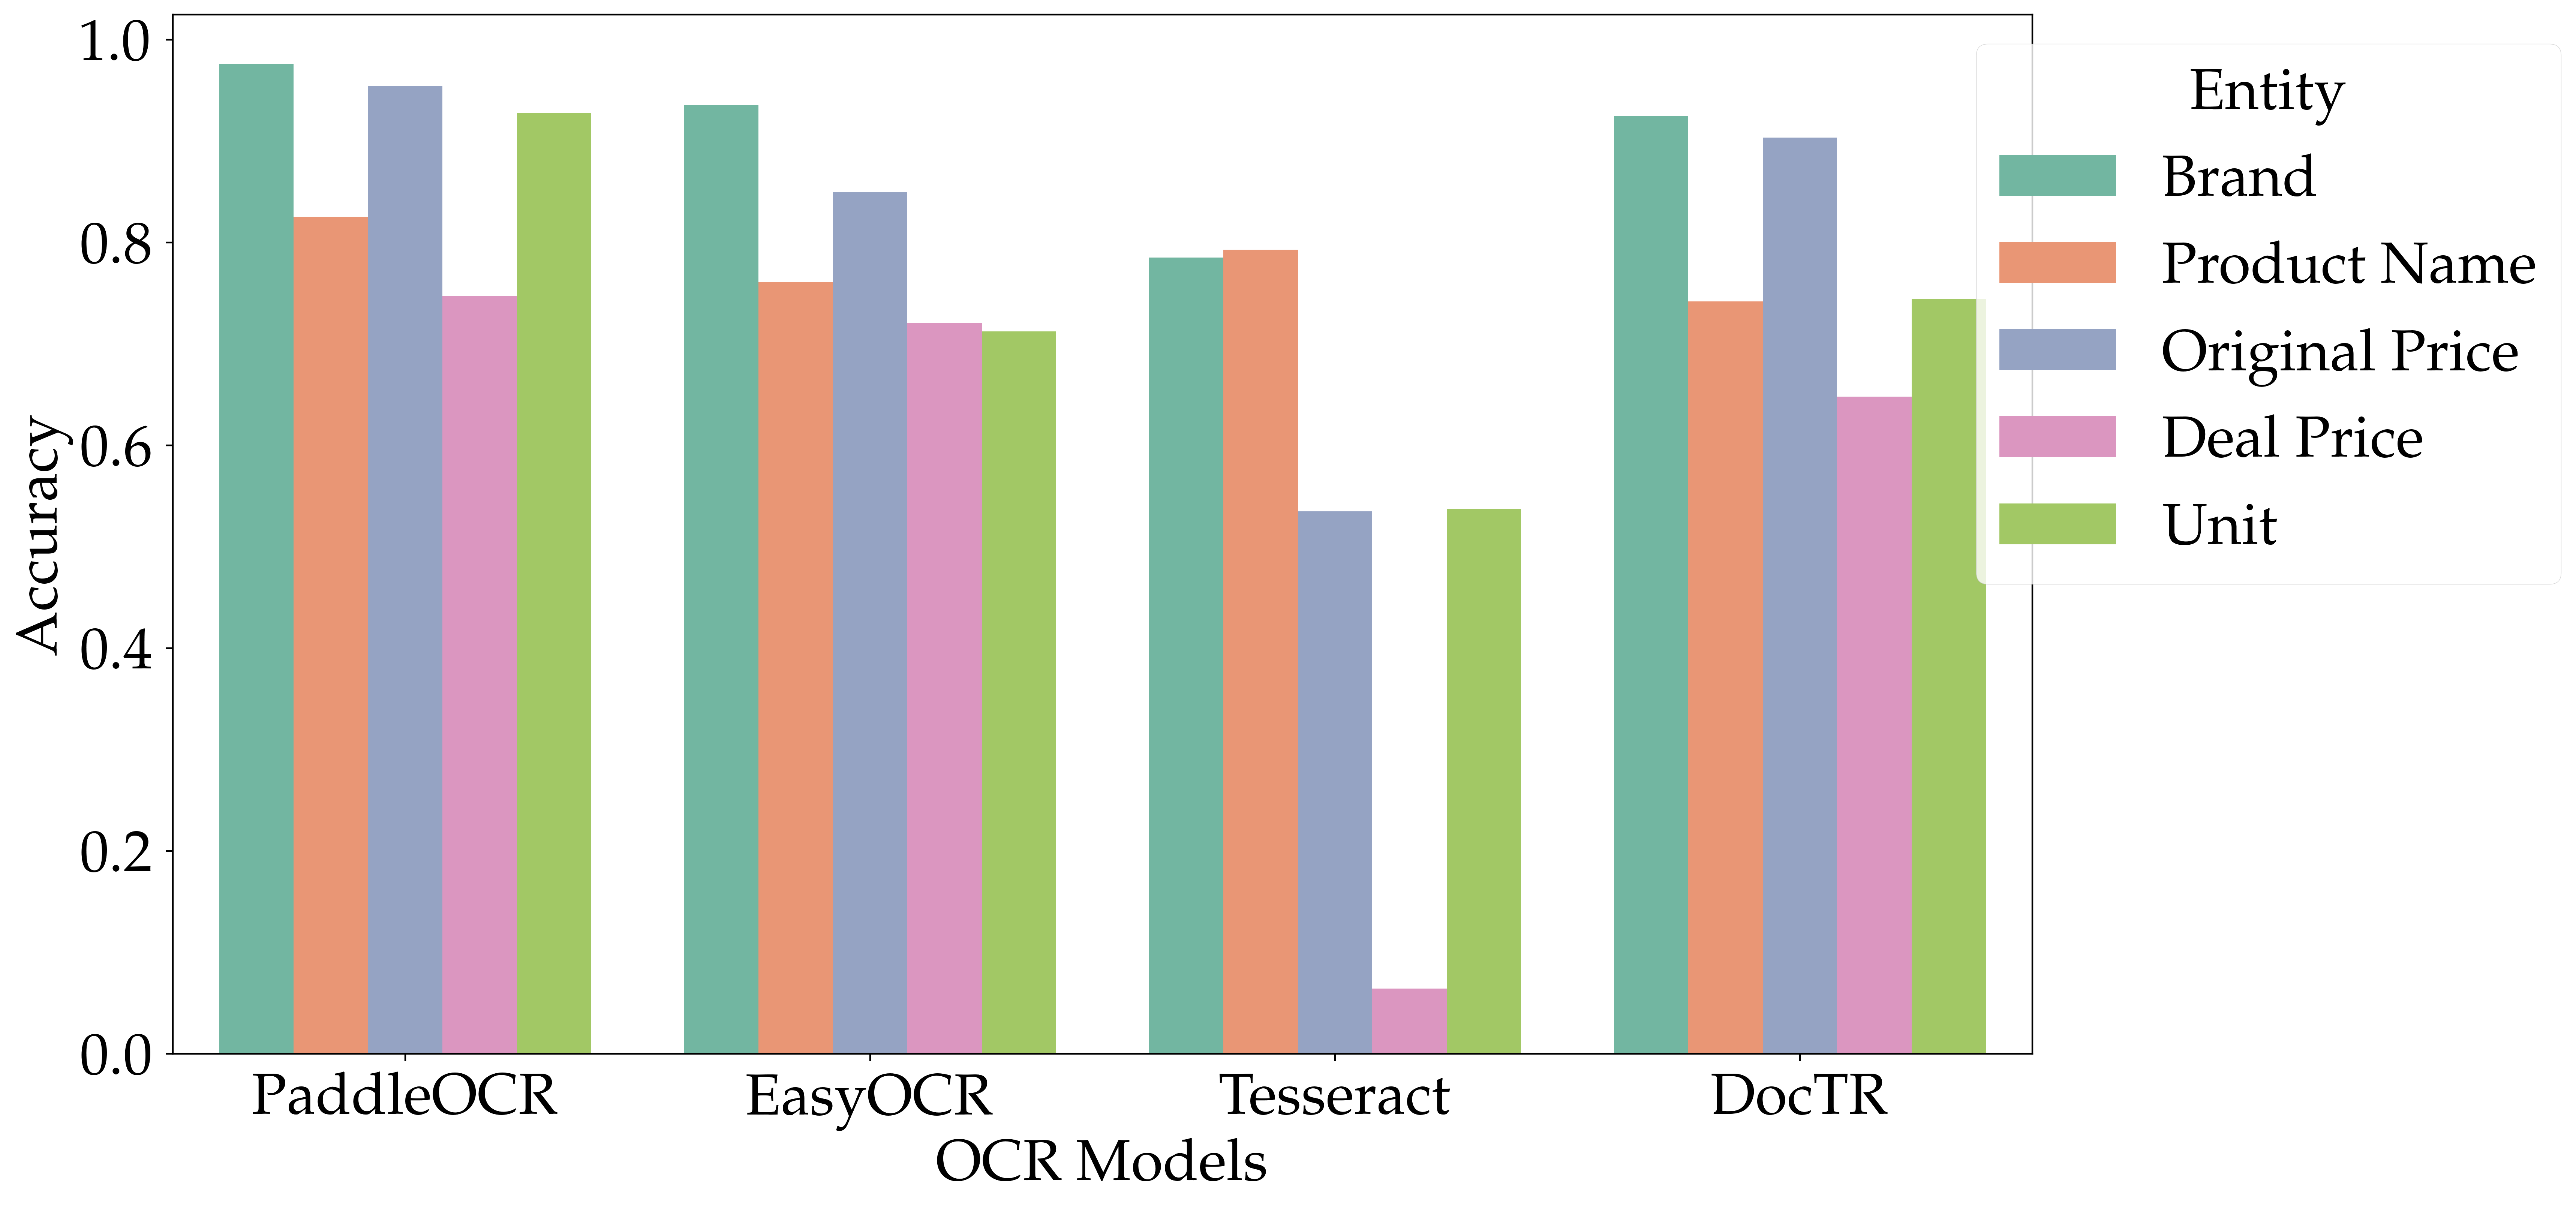
\includegraphics[width=0.5\linewidth]{figures/accuracy_level_4.png} \\
    (c) Level 3 & (d) Level 4 \\[6pt]
    \end{tabular}
    \caption{Per-Entity Accuracy of OCR Models at Different Normalization Levels.}
    \label{fig:eval_ocr_accuracies}
    \end{figure*}

In general, the OCR models exhibit superior performance in extracting words compared to numerical values. This discrepancy is particularly evident in entity-wise accuracy variations. At the baseline level (normalization level 1), the deal price entity consistently shows the lowest accuracy, whereas the brand entity achieves the highest. The accuracy of other entities varies significantly, with PaddleOCR, EasyOCR, and docTR displaying comparable performance, while Tesseract lags behind.

The overall accuracy improves with increasing normalization levels, with normalization level 4 yielding the highest accuracy gains. At this level, Tesseract continues to struggle with deal price recognition, failing in over 90\% of cases. In contrast, the other OCR models achieve accuracies exceeding 70\% across nearly all entity types.

Among the different entities, brand names are consistently recognized with the highest accuracy. This can be attributed to their simpler linguistic structure and distinct visual presentation, as brand names are often bolded or highlighted in promotional material. In contrast, product names tend to have more complex linguistic structures, making exact string matching more challenging.

The recognition of unit information lags behind brand names but remains more accurate than deal prices. The reduced accuracy can be explained by the smaller font size of unit labels, their less prominent placement, and the high variability in unit measurements (e.g., "kg", "g", "Stück"), which complicates recognition.

A significant gap is observed between deal price and original price accuracy. This can be attributed to the typographic differences between the two: deal prices are often emphasized using distinctive fonts and superscripted decimals, making them harder for OCR models to interpret correctly. In contrast, original prices are typically displayed in a standard inline format, which is easier to recognize.

\begin{figure*}[h!]
    \begin{tabular}{cc}
      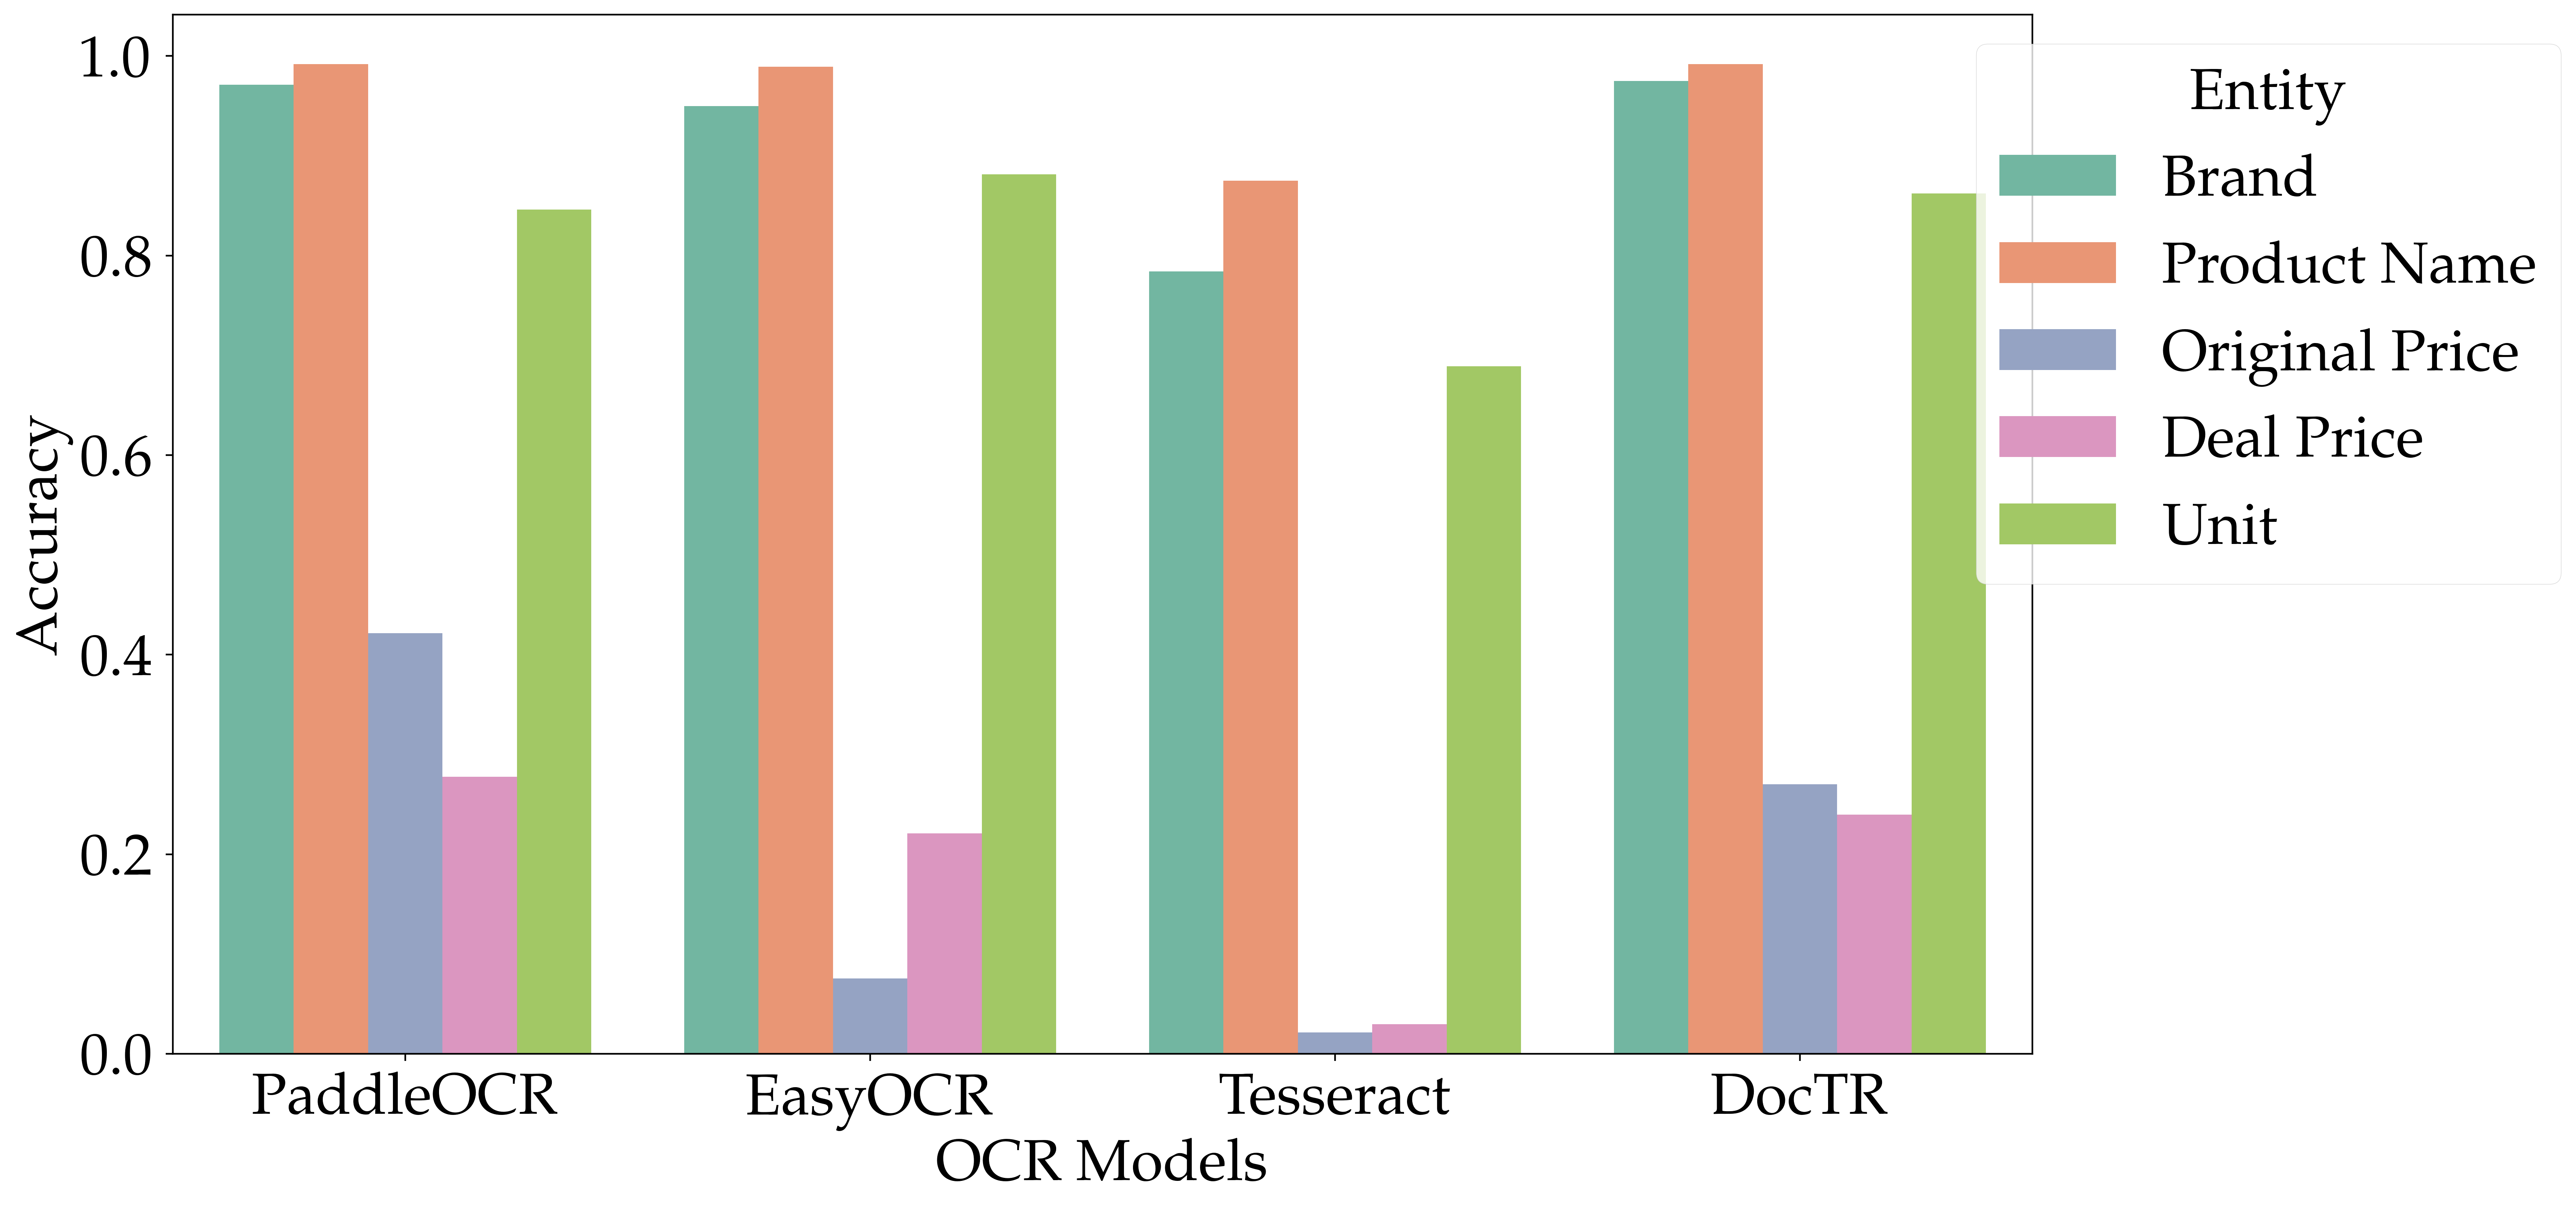
\includegraphics[width=0.5\linewidth]{figures/ngram_accuracy_level_1.png} &   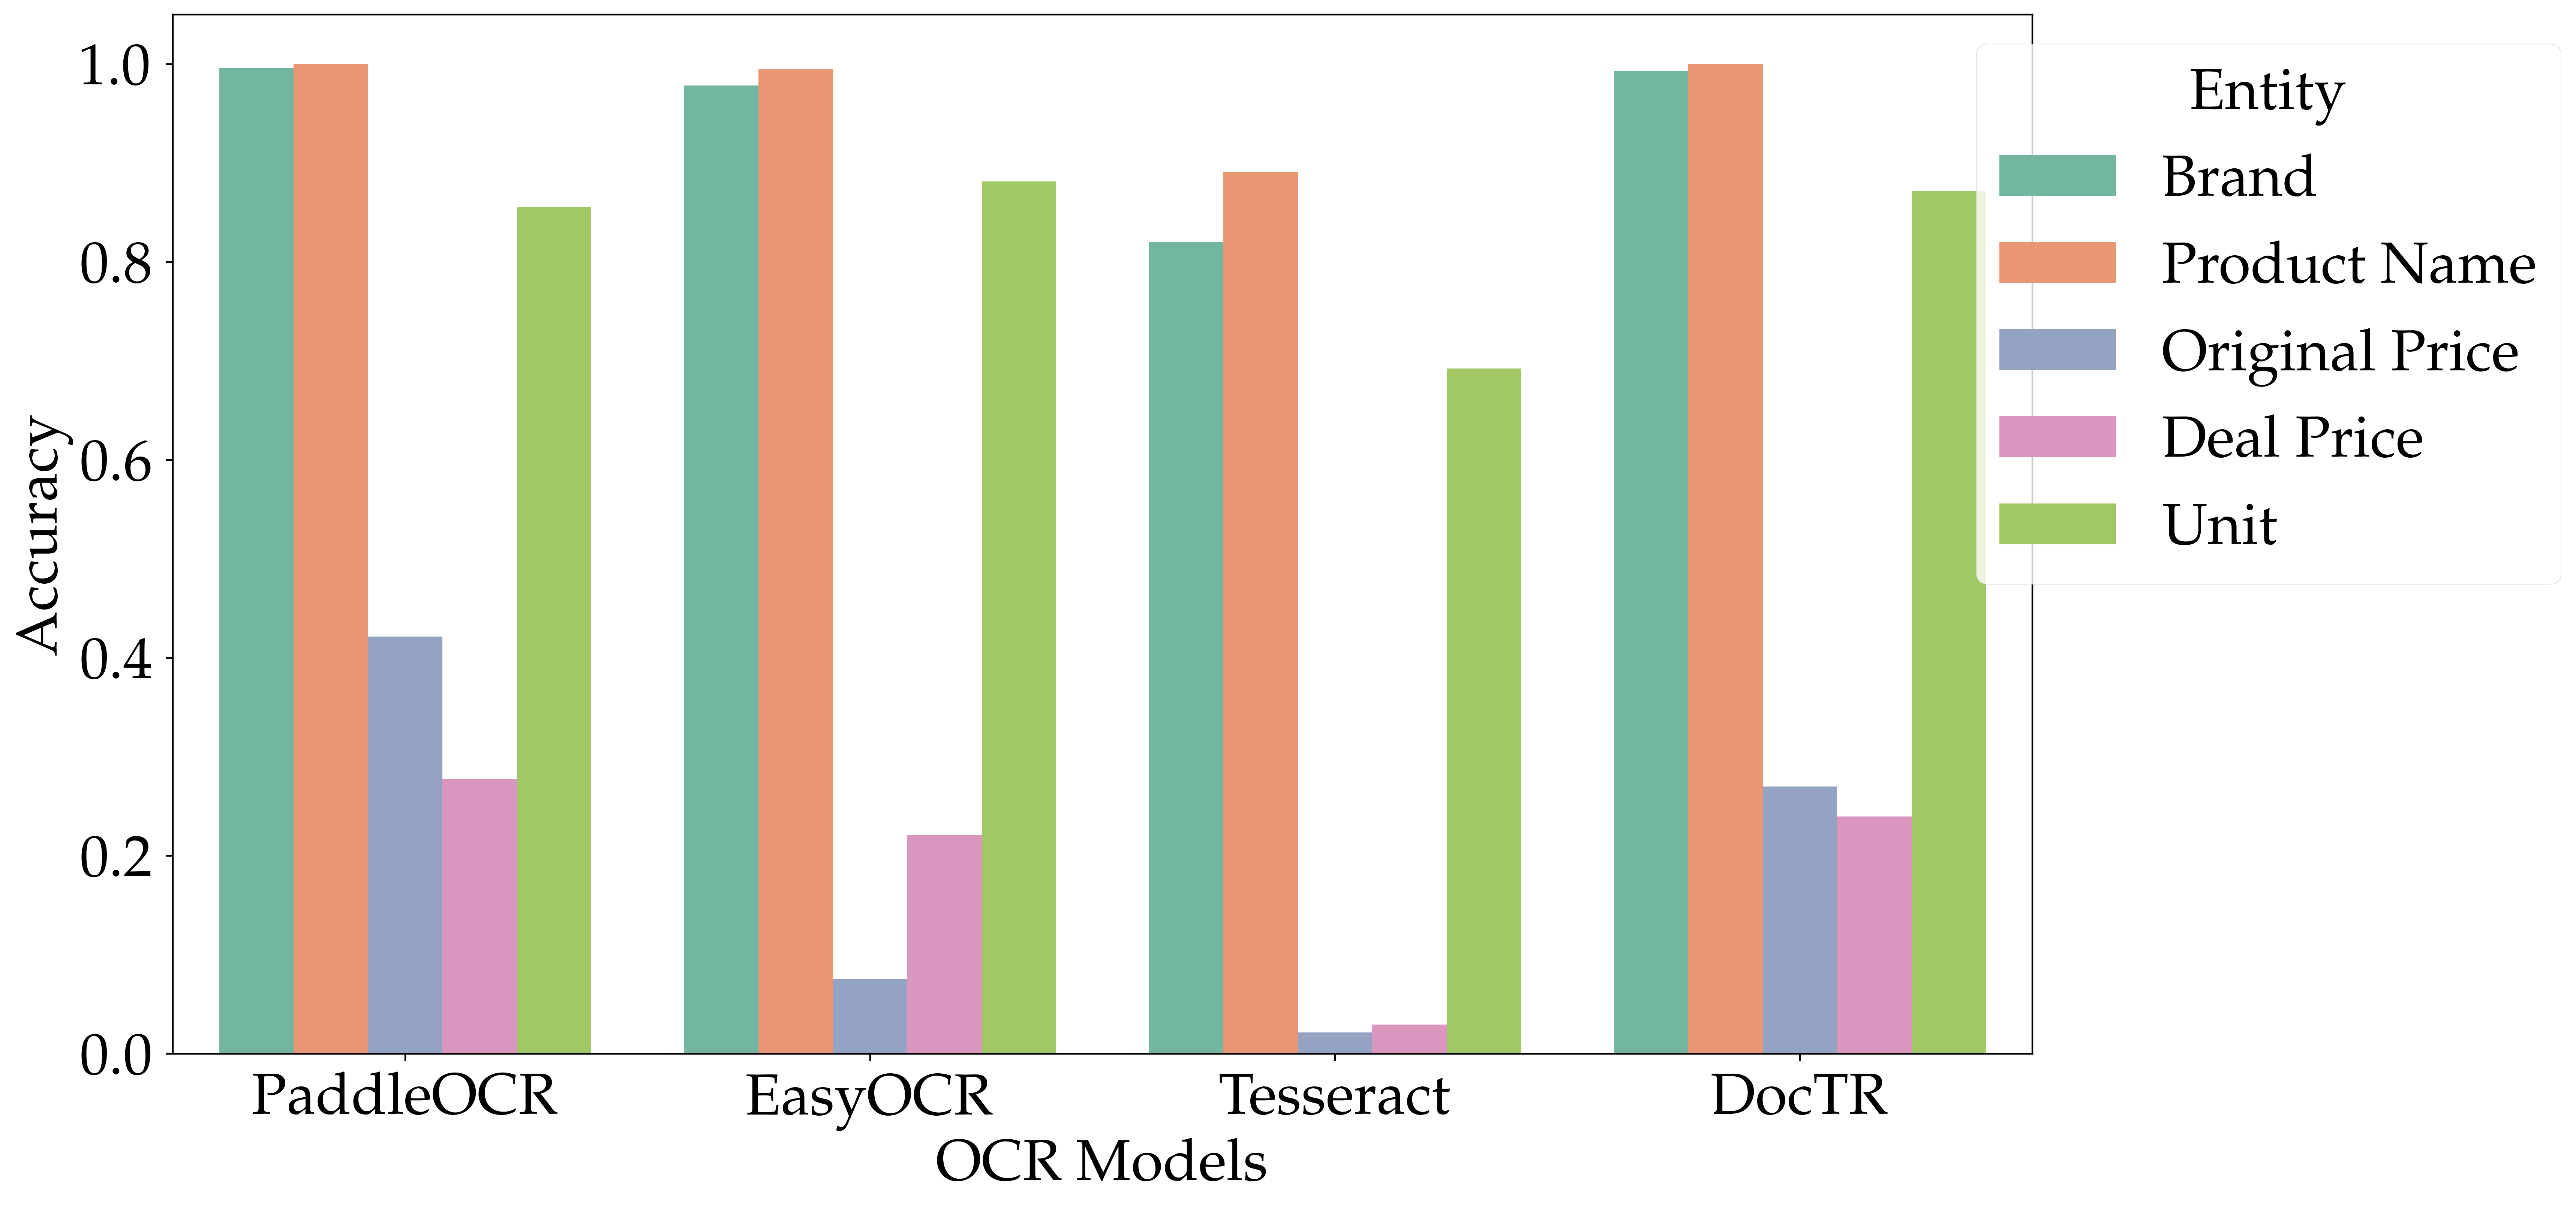
\includegraphics[width=0.5\linewidth]{figures/ngram_accuracy_level_2.png} \\
    (a) Level 1 & (b) Level 2 \\[6pt]
        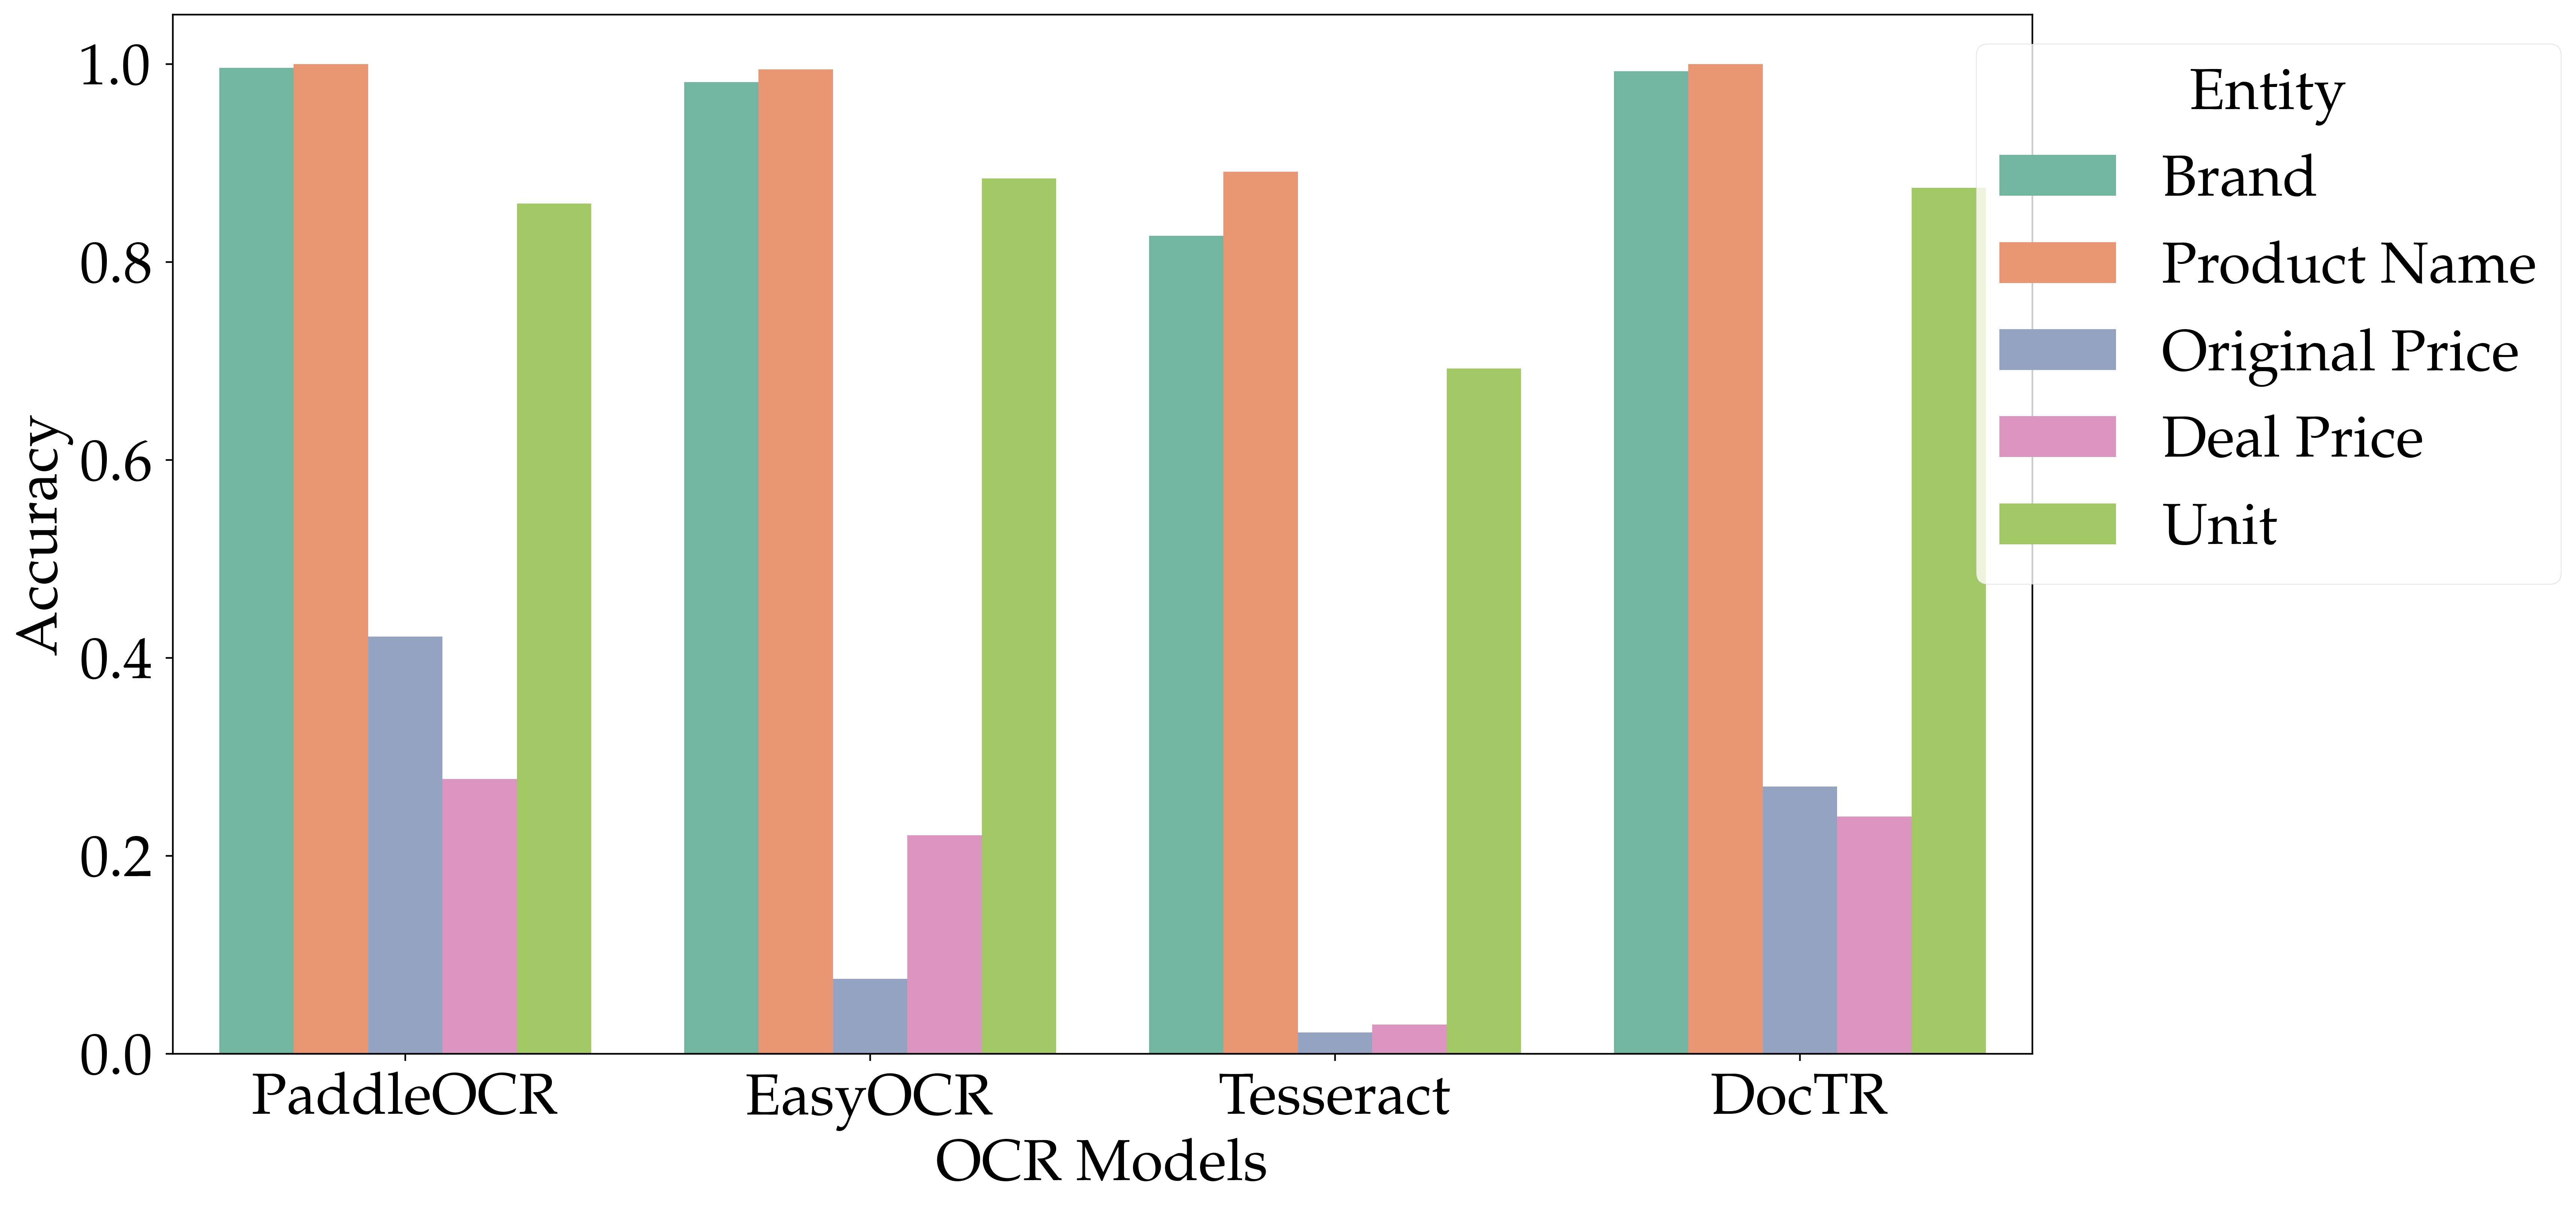
\includegraphics[width=0.5\linewidth]{figures/ngram_accuracy_level_3.png} &   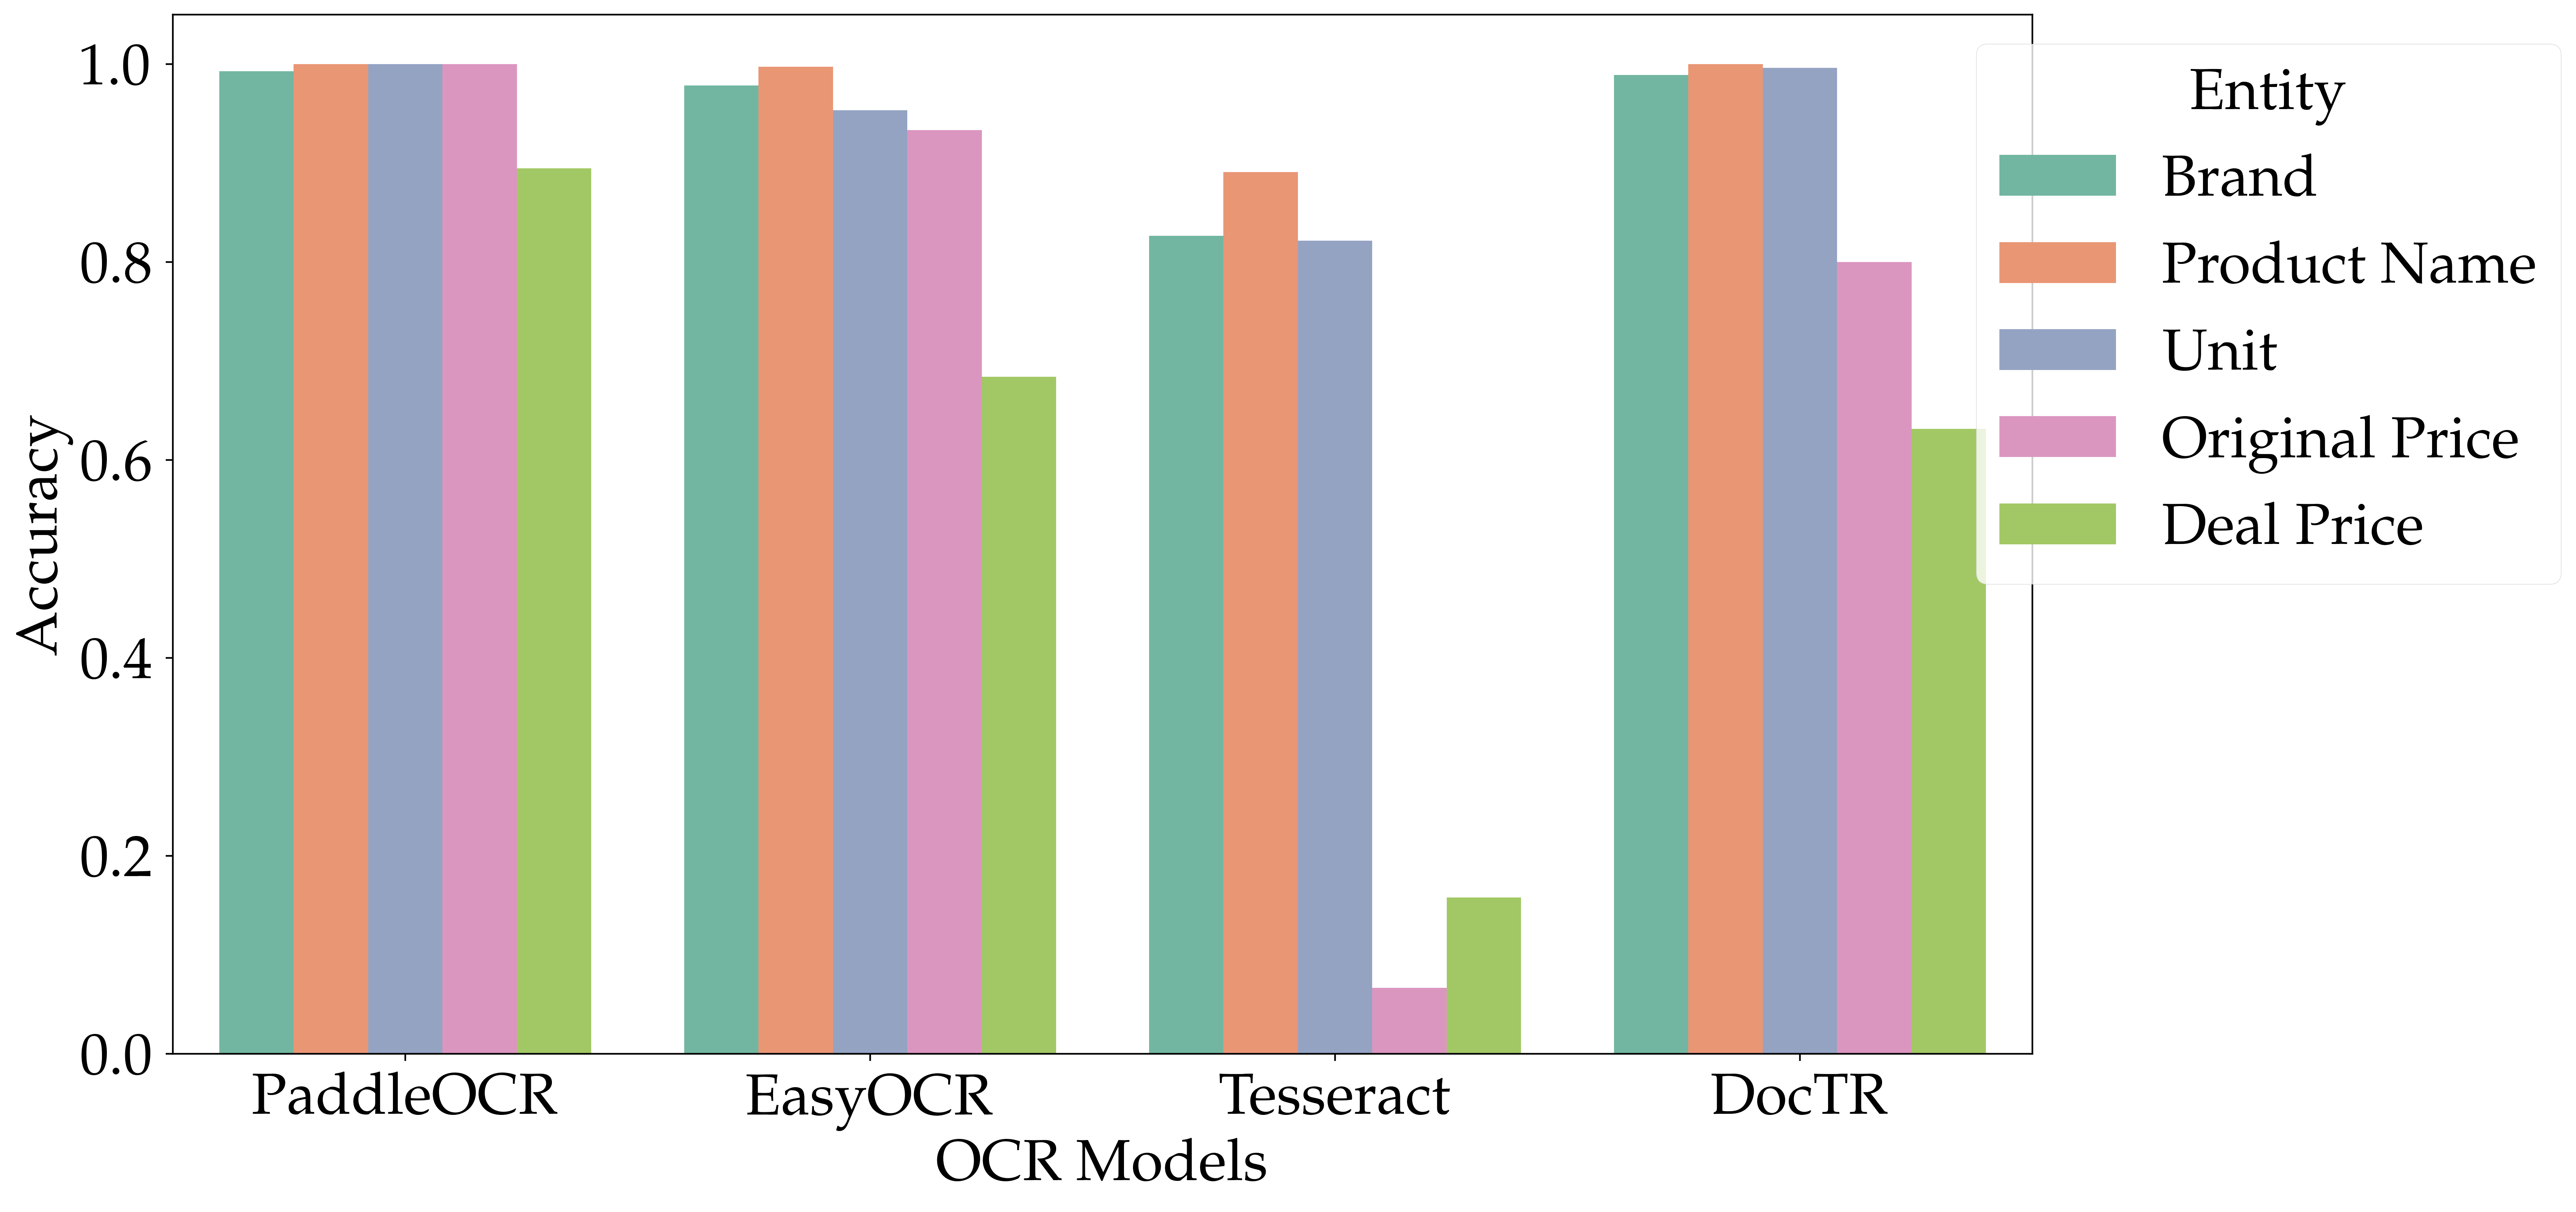
\includegraphics[width=0.5\linewidth]{figures/ngram_accuracy_level_4.png} \\
    (c) Level 3 & (d) Level 4 \\[6pt]
    \end{tabular}
    \caption{Per-Entity N-Gram Accuracy of OCR Models at Different Normalization Levels.}
    \label{fig:eval_ocr_ngram_accuracies}
\end{figure*}

When evaluating n-gram accuracy per-entity in \figref{fig:eval_ocr_ngram_accuracies}, the results reveal a similar trend to per-entity accuracy. When comparing the OCR models, PaddleOCR consistently outperforms the other models especially in the price extractions while Tesseract lacks behind in all entities.

The most significant observation is that the deal price and original price exhibit in lower normalization levels significantly worse accuracies. Since the length of n-gram sequences increase superlinearly, longer entity values, precisely the brand and product name, more likely achieve higher accuracies, which is also reflected in the results.

At the highest normalization level, most models achieve 100\% or close to 100\% n-gram accuracy in the majority of entites. Additionally, here the discrepancy of Tesseract is most visible, where it cannot nearly achieve comparable scores. Also, one can observe that the unit entity drops significantly at level 4 across all models. This can be attributed to the high variability in unit measurements, which makes it challenging to match the exact n-grams.


% EXPERIMENT: OCR+LLM
\subsubsection{Hybrid-OCR+LLM Performance}

In addition to evaluating the OCR capabilities, the performance of OCR models was assessed in conjunction with LLMs. The primary objectives were to determine the most effective OCR-LLM combination for information extraction and to evaluate the impact of different OCR models on the LLM's performance.

All 372 samples of the Leaflet-IE dataset were used for evaluation. It is assumed that neither the OCR models nor the LLMs have previously encountered this data, similar to the OCR evaluation. Since the task is to extract structured information, the evaluation metrics were adapted to reflect the performance of the OCR-LLM combination in generating key-value mappings. The evaluation metrics include:
\begin{itemize}
    \item \textbf{Accuracy (Per Entity):} Measures the accuracy (of each extracted entity).
    \item \textbf{Levenshtein Distance:} Calculates the distance between the prediction and the ground truth.
\end{itemize}

The LLMs were prompted to extract entities from the OCR output. The specific prompt used can be found in \secref{app:llm_prompt}.

\paragraph{Models Evaluated:}
\begin{itemize}
    \item \textbf{Llama 3.1 [8b, Q4]}: \texttt{llama3.1\_8b} \cite{touvron2023},
    \item \textbf{Qwen 2.5 [1.5b, Q8]}: \texttt{qwen2.5\_1.5b-instruct-q8\_0} \cite{qwen2025},
    \item \textbf{Llama 3.2 [3b, Q8]}: \texttt{llama3.2\_3b-instruct-q8\_0} \cite{touvron2023},
    \item \textbf{Qwen 2.5 [7b, Q4]}: \texttt{qwen2.5\_7b} \cite{qwen2025}.
\end{itemize}
where the LLM name and version is additionally specified through the model size (in billions of parameters) and the quantization level.

To avoid confusion with the normalization used in the OCR experiment, the OCR results were kept raw, as normalization may remove valuable information. The LLMs are expected to handle such inconsistencies and errors in the input. Instead, here the entity values were evaluated in both raw form and with a normalization applied for the comparability between the LLM prediction and the ground truth value. The normalization procedure includes usual character replacements and filtering based on linguistic artifacts commonly encountered in OCR errors. The specific normalization procedure can be found in \secref{app:ocr_llm_normalization}.
\paragraph{Results:}
The entity-averaged accuracies and Levenshtein distances for the raw OCR output are depicted in Figures \ref{fig:eval_ocr_llm_accuracies_avg} and \ref{fig:eval_ocr_llm_levdist_avg}, respectively.

\begin{figure*}[h!]
    \centering
    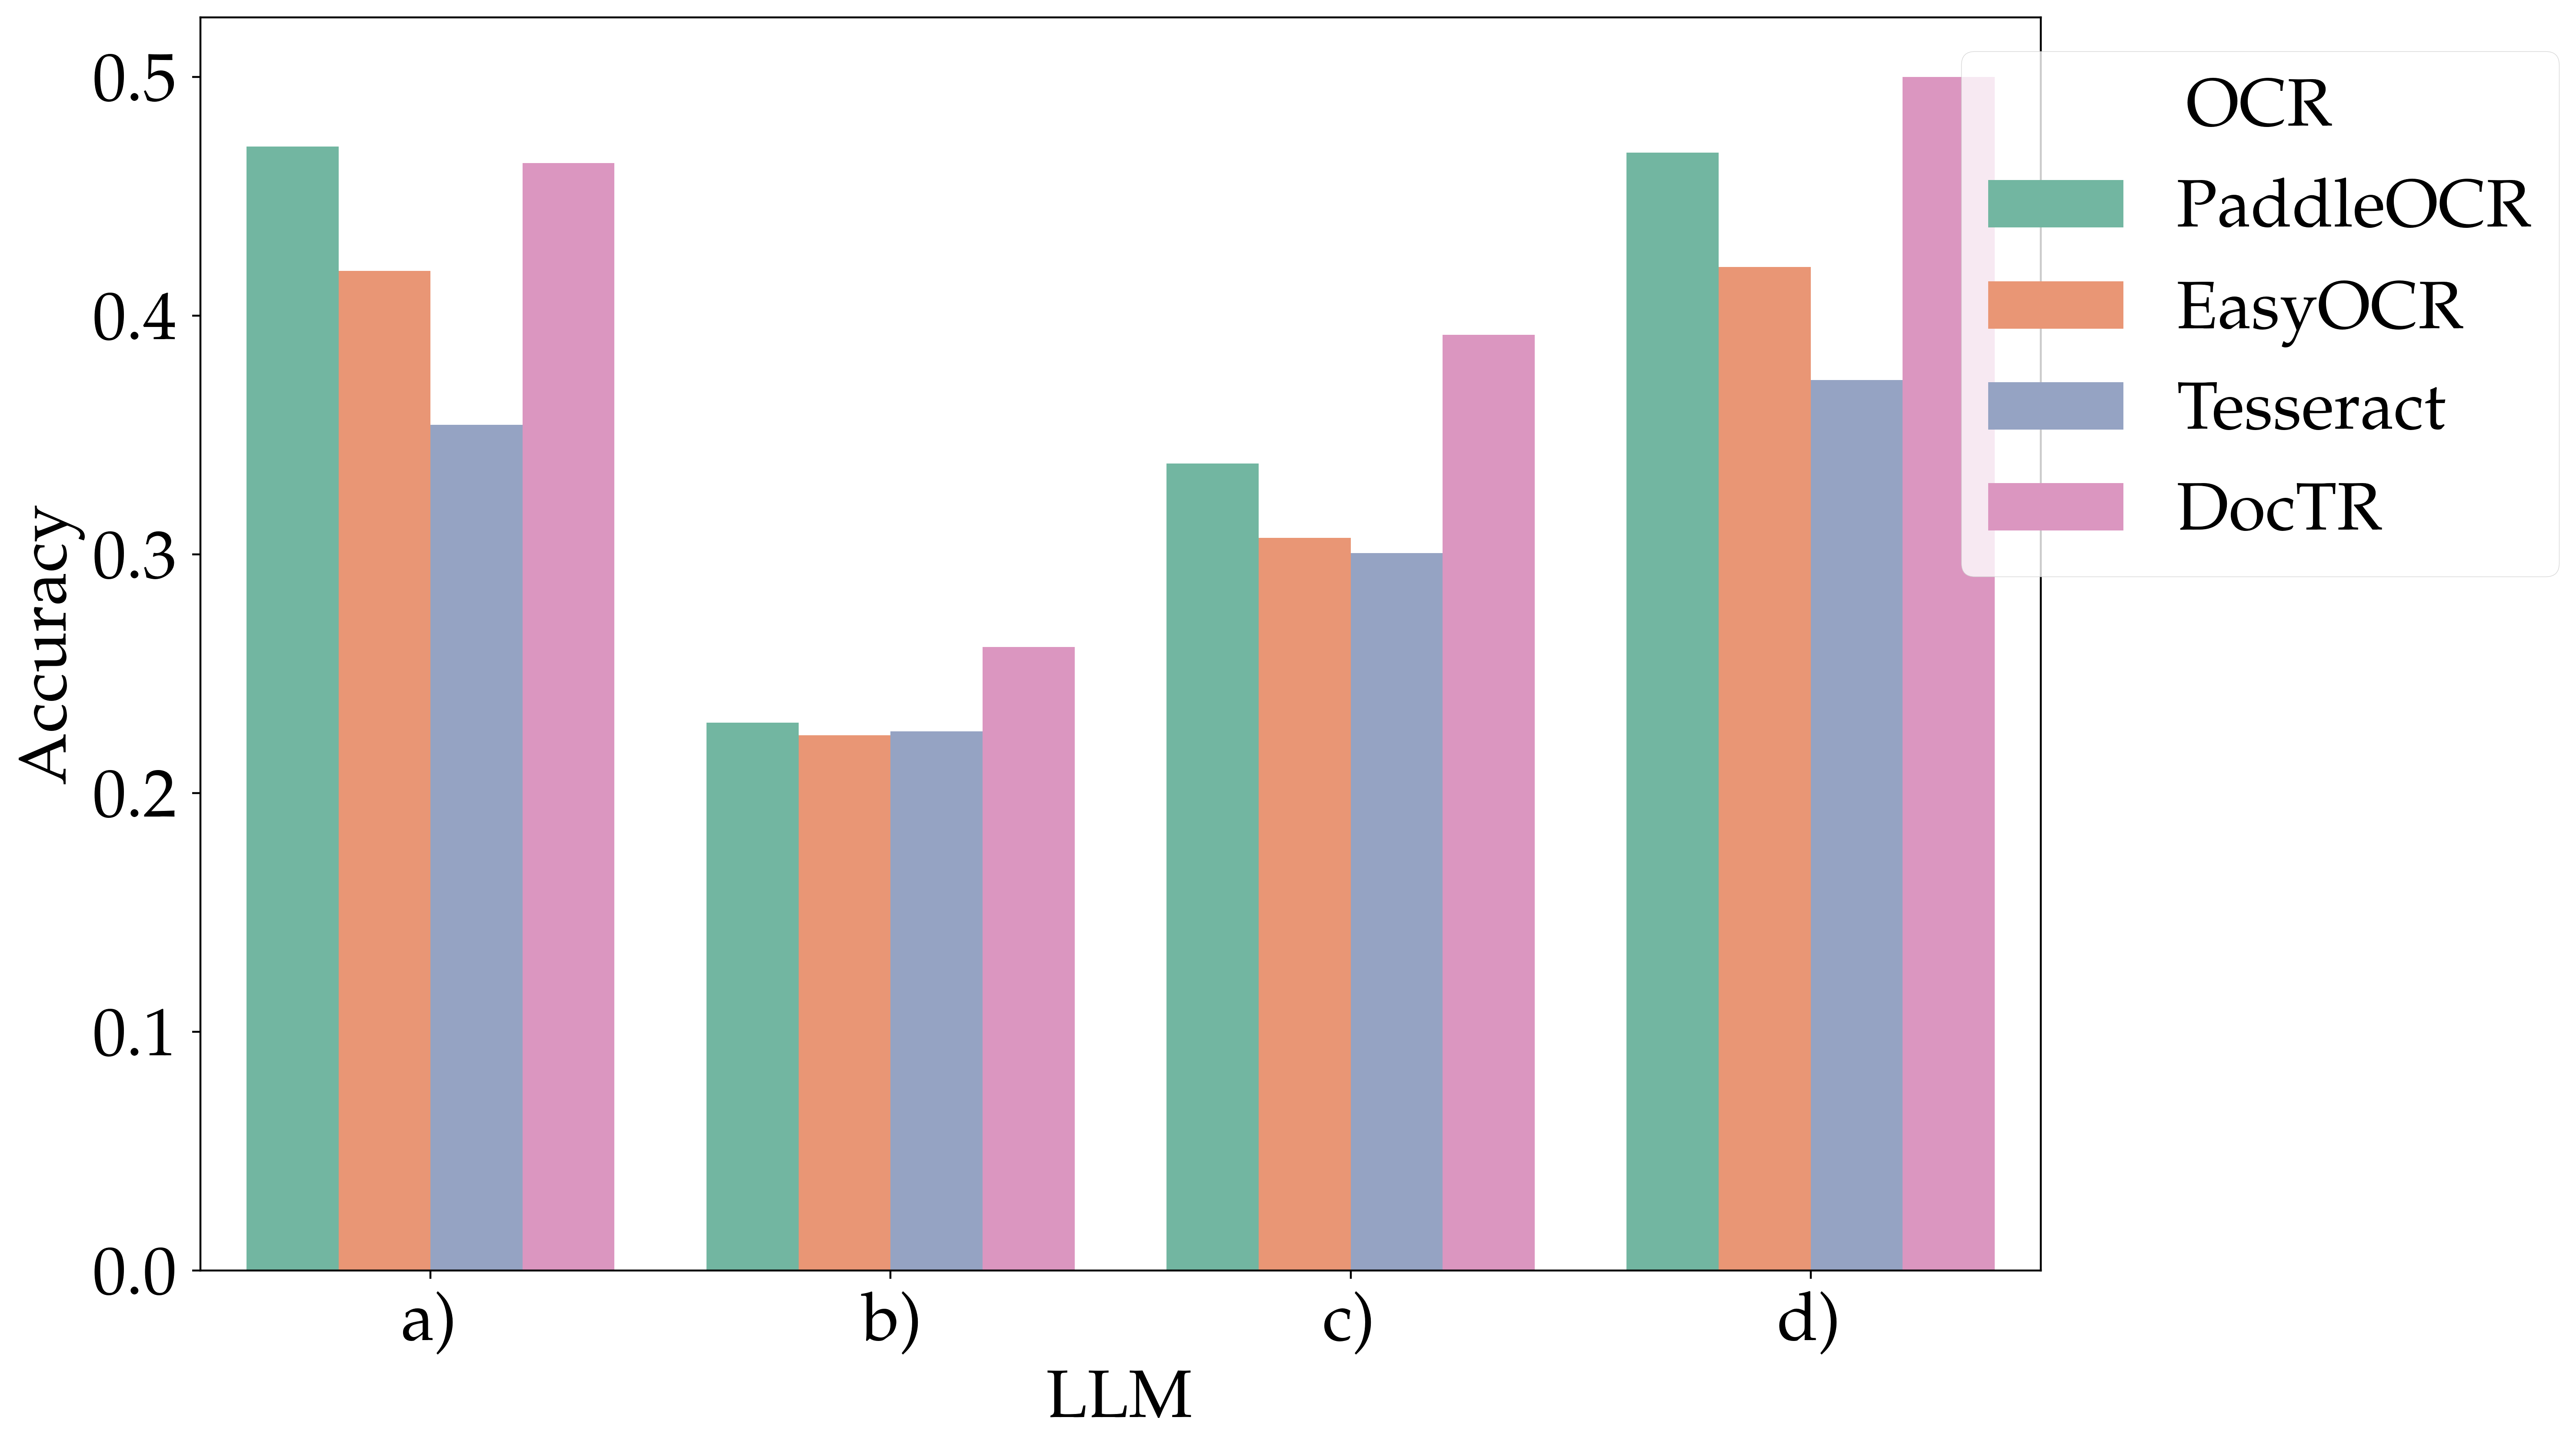
\includegraphics[width=0.8\linewidth]{figures/avg_accuracies.png}
    \caption{Entity-Averaged Accuracy of LLM Models per Raw OCR Output. a: Llama 3.1 [8b, Q4], b: Qwen 2.5 [1.5b, Q8], c: Llama 3.2 [3b, Q8], d: Qwen 2.5 [7b, Q4].}
    \label{fig:eval_ocr_llm_accuracies_avg}
\end{figure*}

The averaged accuracies reveal that a higher number of parameters is more beneficial for the LLMs in this task than a higher quantization level. Specifically, the Llama 3.1:8b and Qwen 2.5:7b models achieve significantly higher accuracy scores than their counterparts with a lower number of parameters. Qwen 2.5:1.5b in Q8 performs worse than Llama 3.2:3b in Q8, but Qwen 2.5:7b in Q4 is overall the best. These differences can be attributed to multiple factors, such as the pre-training data of the models, the model architecture, or the prompt used to extract the entities. DocTR and PaddleOCR achieve equal or better results than Tesseract and EasyOCR. Specifically, Tesseract consistently performs the worst among the evaluated models.

\begin{figure*}[h!]
    \centering
    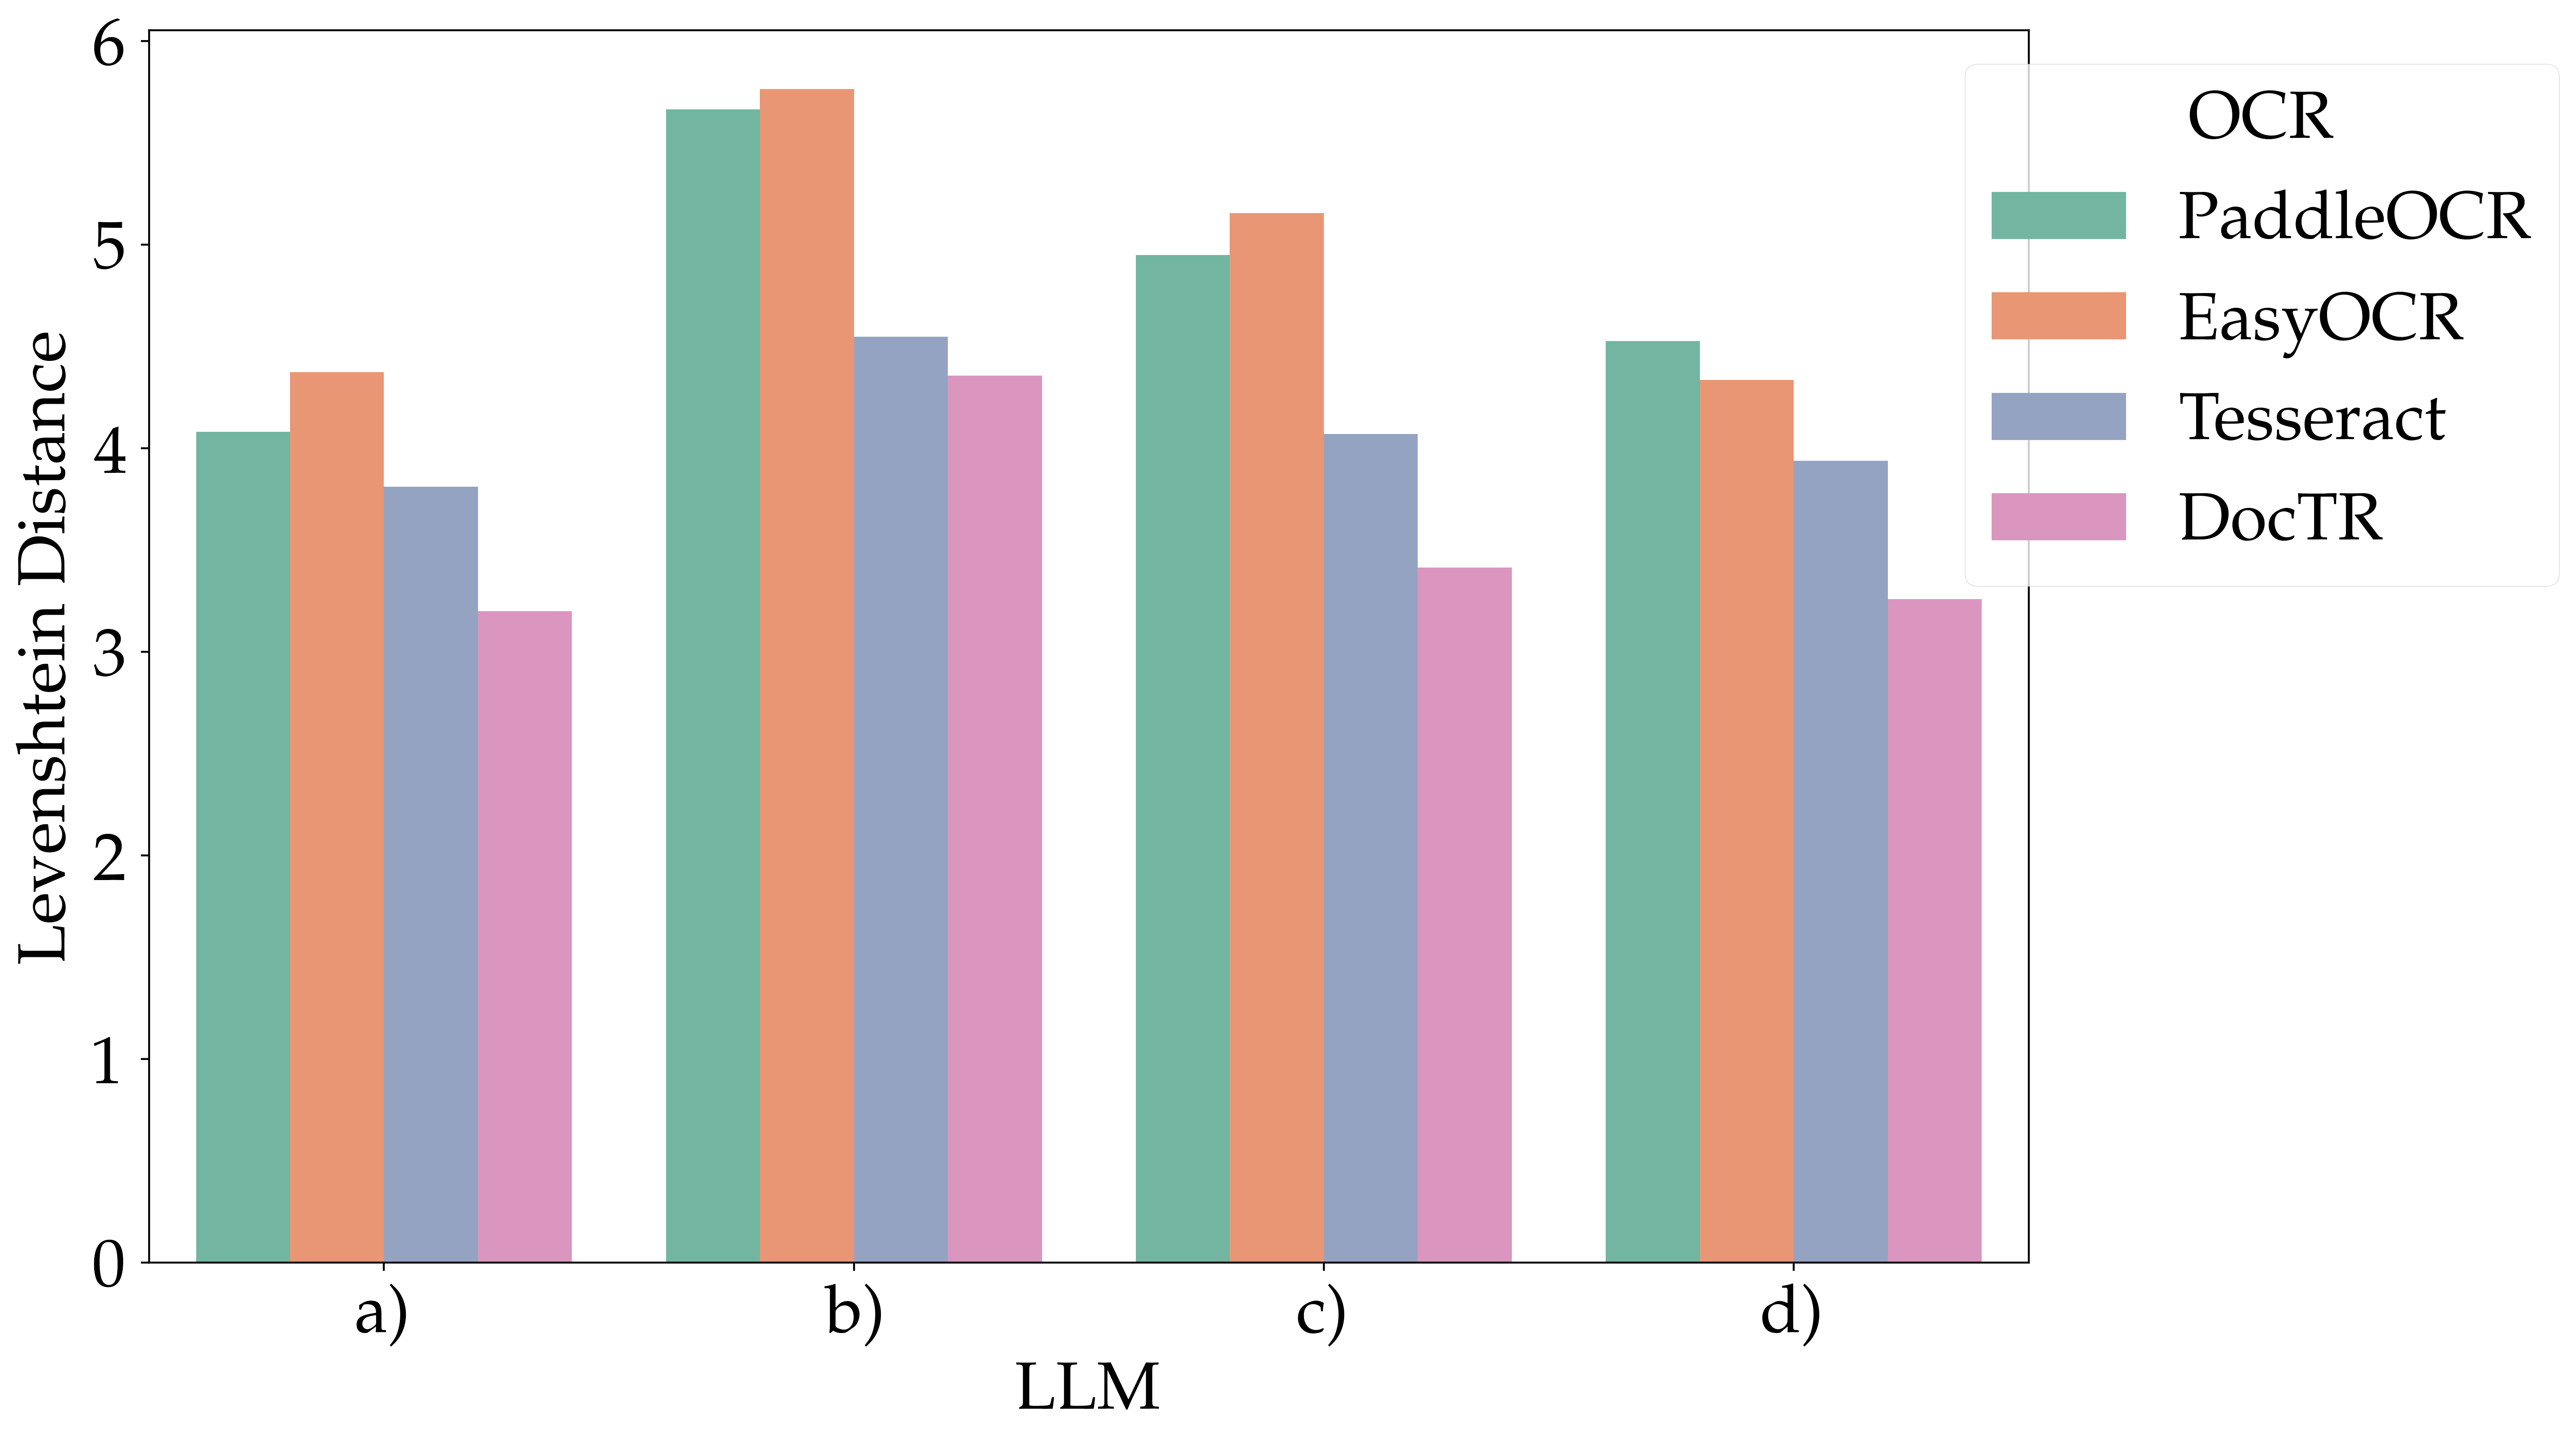
\includegraphics[width=0.8\linewidth]{figures/avg_levdistances.png}
    \caption{Entity-Averaged Levenshtein Distance of OCR-LLM Models (Raw OCR Output). a: Llama 3.1 [8b, Q4], b: Qwen 2.5 [1.5b, Q8], c: Llama 3.2 [3b, Q8], d: Qwen 2.5 [7b, Q4].}
    \label{fig:eval_ocr_llm_levdist_avg}
\end{figure*}

When regarding the levenshtein distances, the results show similar trends. DocTR delivers by far the best OCR input across all OCR models. Suprisingly, Tesseract achieves lower levenshtein distances than PaddleOCR and EasyOCR, with EasyOCR being the worst across all models. This could be due to the fact that Tesseract delivers more often slightly wrong but still similar results, while EasyOCR delivers less often wrong but more different results. The LLMs show similar trends as in the accuracy evaluation, but Llama 3.1:8b now slightly outperforms Qwen 2.5:7b. The differences between the LLMs are less pronounced than in the accuracy evaluation, which can be attributed to the unnormalized levenshtein distance calculation used. \secref{app:ocr_llm_results} provides further results on entity-level accuracies and levenshtein distances for each OCR-LLM combination.

\subsection{Donut Fine-Tuning Performance}
The experiment aims to evaluate the fine-tuning performance of the Vision Encoder-Decoder model, Donut, pretrained on the CORD dataset, to determine its capability in extracting end-to-end information from supermarket leaflet deal images. Conducted on an NVIDIA RTX 4080 (Station 1), the model has a vocabulary size of 57,580 and 201M parameters. The training configuration includes 10 epochs, validation performed every epoch, gradient clipping at 2.0, 800 training samples per epoch, a learning rate of 8e-6, batch sizes of 16 for both training and validation, 400 warmup steps, and 16-bit mixed precision.

\indent{\textbf{Results}.} The training and validation losses of Donut during fine-tuning are depicted in \figref{fig:donut_loss}. The training loss decreases rapidly, while the validation loss remains high, indicating overfitting. The overfitting is likely due to the limited number of deal layouts in the training data, which restricts the model's ability to generalize to unseen layouts. This issue is visually less pronounced, as the text is relatively consistent across deals, but textually, the model struggles to generalize due to the diverse language and layout variations. Another problem is that the model is not pretrained on the German language, which may further hinder its performance.

\begin{figure*}[h!]
    \begin{tabular}{cc}
    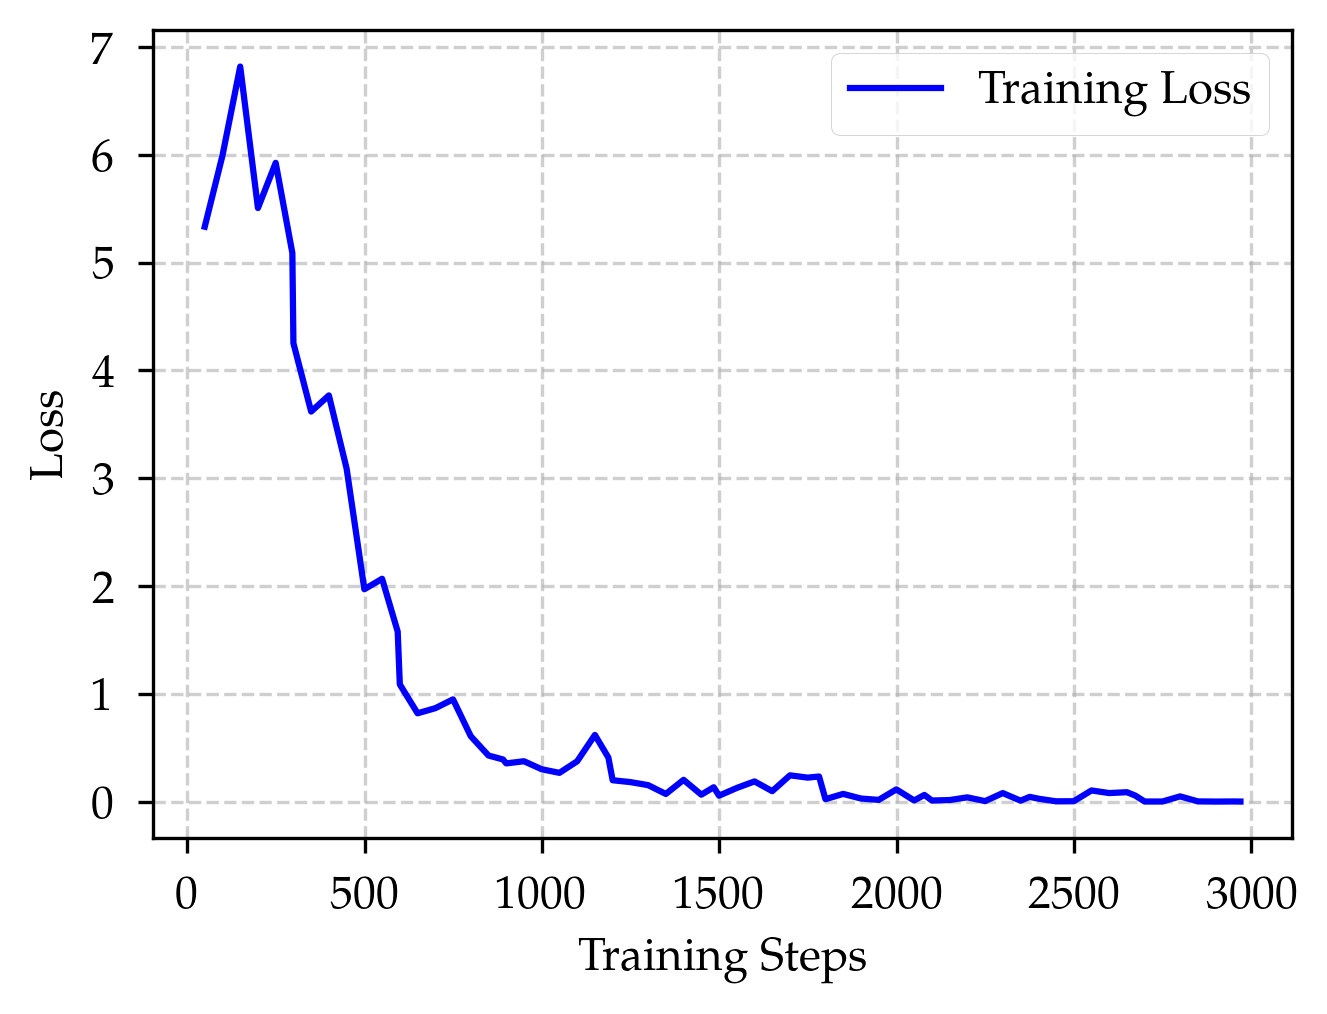
\includegraphics[width=0.4\linewidth]{figures/donut_train_loss.png} &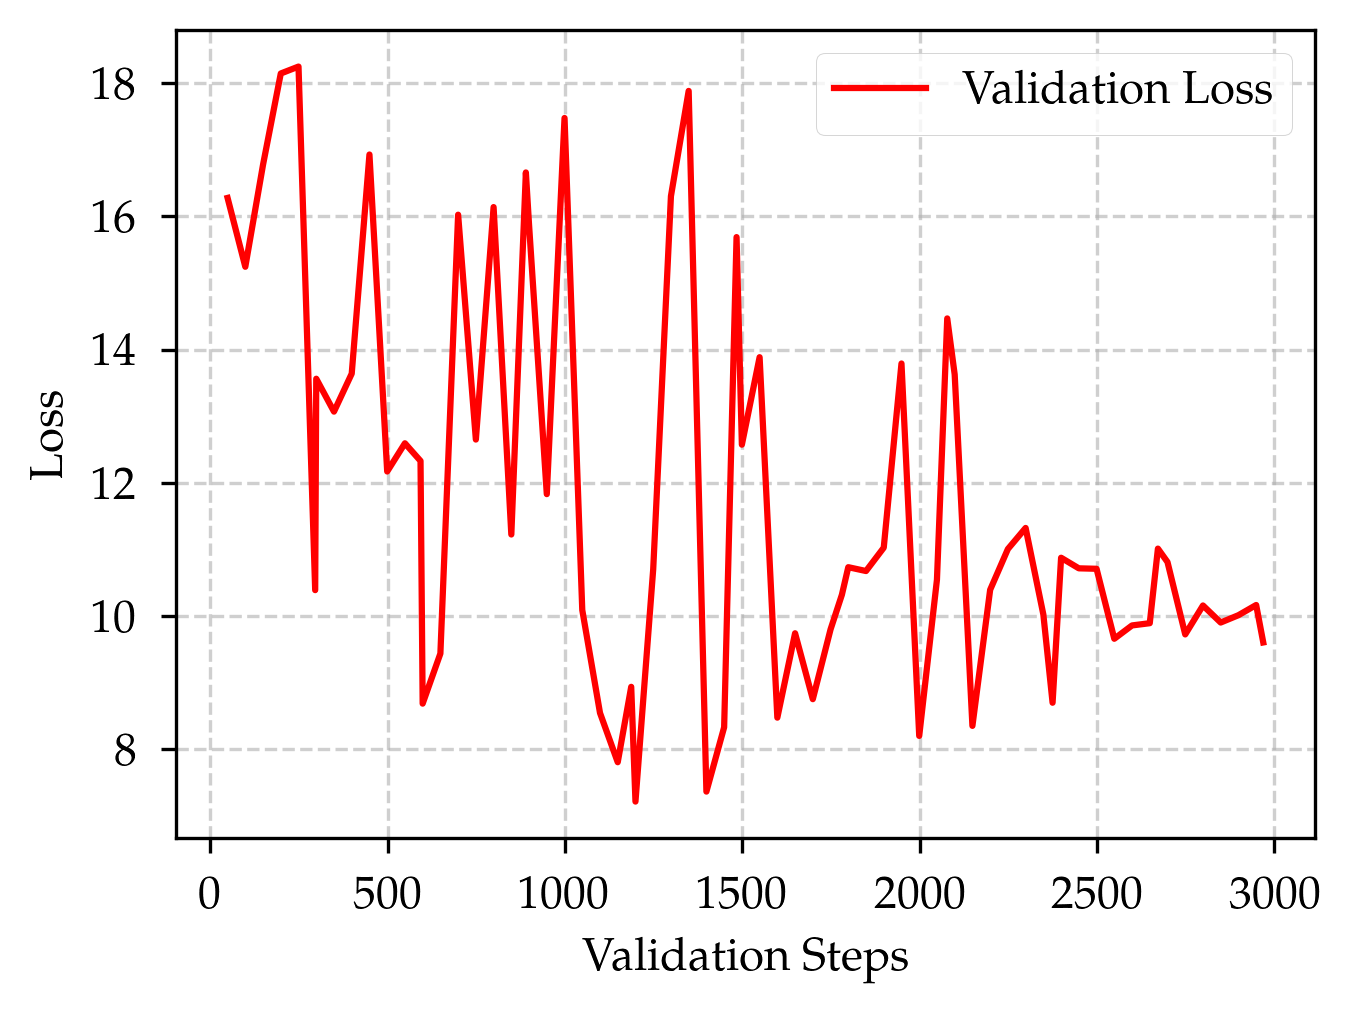
\includegraphics[width=0.4\linewidth]{figures/donut_val_loss.png} \\
    (a) Training Loss & (b) Validation Loss \\[6pt]
    \end{tabular}
    \caption{Training and Validation Loss of Donut during Fine-Tuning.}
    \label{fig:donut_loss}
\end{figure*}


\subsection{Comparison of Hybrid OCR+LLM, Donut, and LVLM}

This section presents a comparative evaluation of a hybrid OCR+LLM pipeline against end-to-end models, specifically Donut and LVLMs, for IE from supermarket deals. The assessment focuses on model performance using the best OCR+LLM configuration and two end-to-end approaches.

\subsubsection{Experimental Setup}
% TODO: Remove \subsection{Comparison of Hybrid OCR+LLM, Donut, and LVLM} because it is the same as the following? (ILYI)
The evaluation framework was designed to compare the performance of three distinct model categories: OCR+LLM pipelines, end-to-end Vision Encoder-Decoder models, and LVLMs. For the OCR+LLM approach, DocTR served as the OCR engine, paired with Qwen 2.5-7B and LLaMA 3.1-8B as the large language models, selected for their comparable performance. The Donut model, an end-to-end Vision Encoder-Decoder architecture optimized for document understanding, was included to assess its capabilities in handling structured document data. Additionally, MiniCPM-V \cite{yao2024} and LLaMA 3.2-Vision \cite{touvron2023} were chosen as representative LVLMs to evaluate their multimodal reasoning abilities.

The evaluation was conducted on the Leaflet-IE validation subset, ensuring a fair comparison across the models. Donut had already been fine-tuned on the training subset. The same metrics, accuracy and Levenshtein distance, were employed to assess model performance. To maintain consistency, the same normalization approach used in the OCR+LLM evaluation was applied uniformly to both model predictions and ground truth values. This setup ensured a rigorous and standardized comparison of model performance across the selected metrics.

\paragraph{Per-Entity Accuracy and Levenshtein Distance}  
The evaluation of per-entity accuracy and Levenshtein distance reveals distinct performance patterns across models, as illustrated in \figref{fig:eval_final_acc_raw} and \figref{fig:eval_final_levdis_raw}. Without normalization, the OCR+LLM pipeline performed significantly worse than Donut and LVLMs, achieving near 0\% accuracy for original and deal price entities, while LVLMs outperformed all models, particularly in price extraction, due to their ability to leverage spatial and contextual cues. Donut trailed closely but showed a notable drop in brand recognition accuracy. Levenshtein distance metrics mirrored these trends, with LVLMs and Donut exhibiting low distances, indicating high precision, while OCR+LLM struggled, especially with brand names, which consistently had the highest distances across models.  

\begin{figure*}[h!]
    \centering
    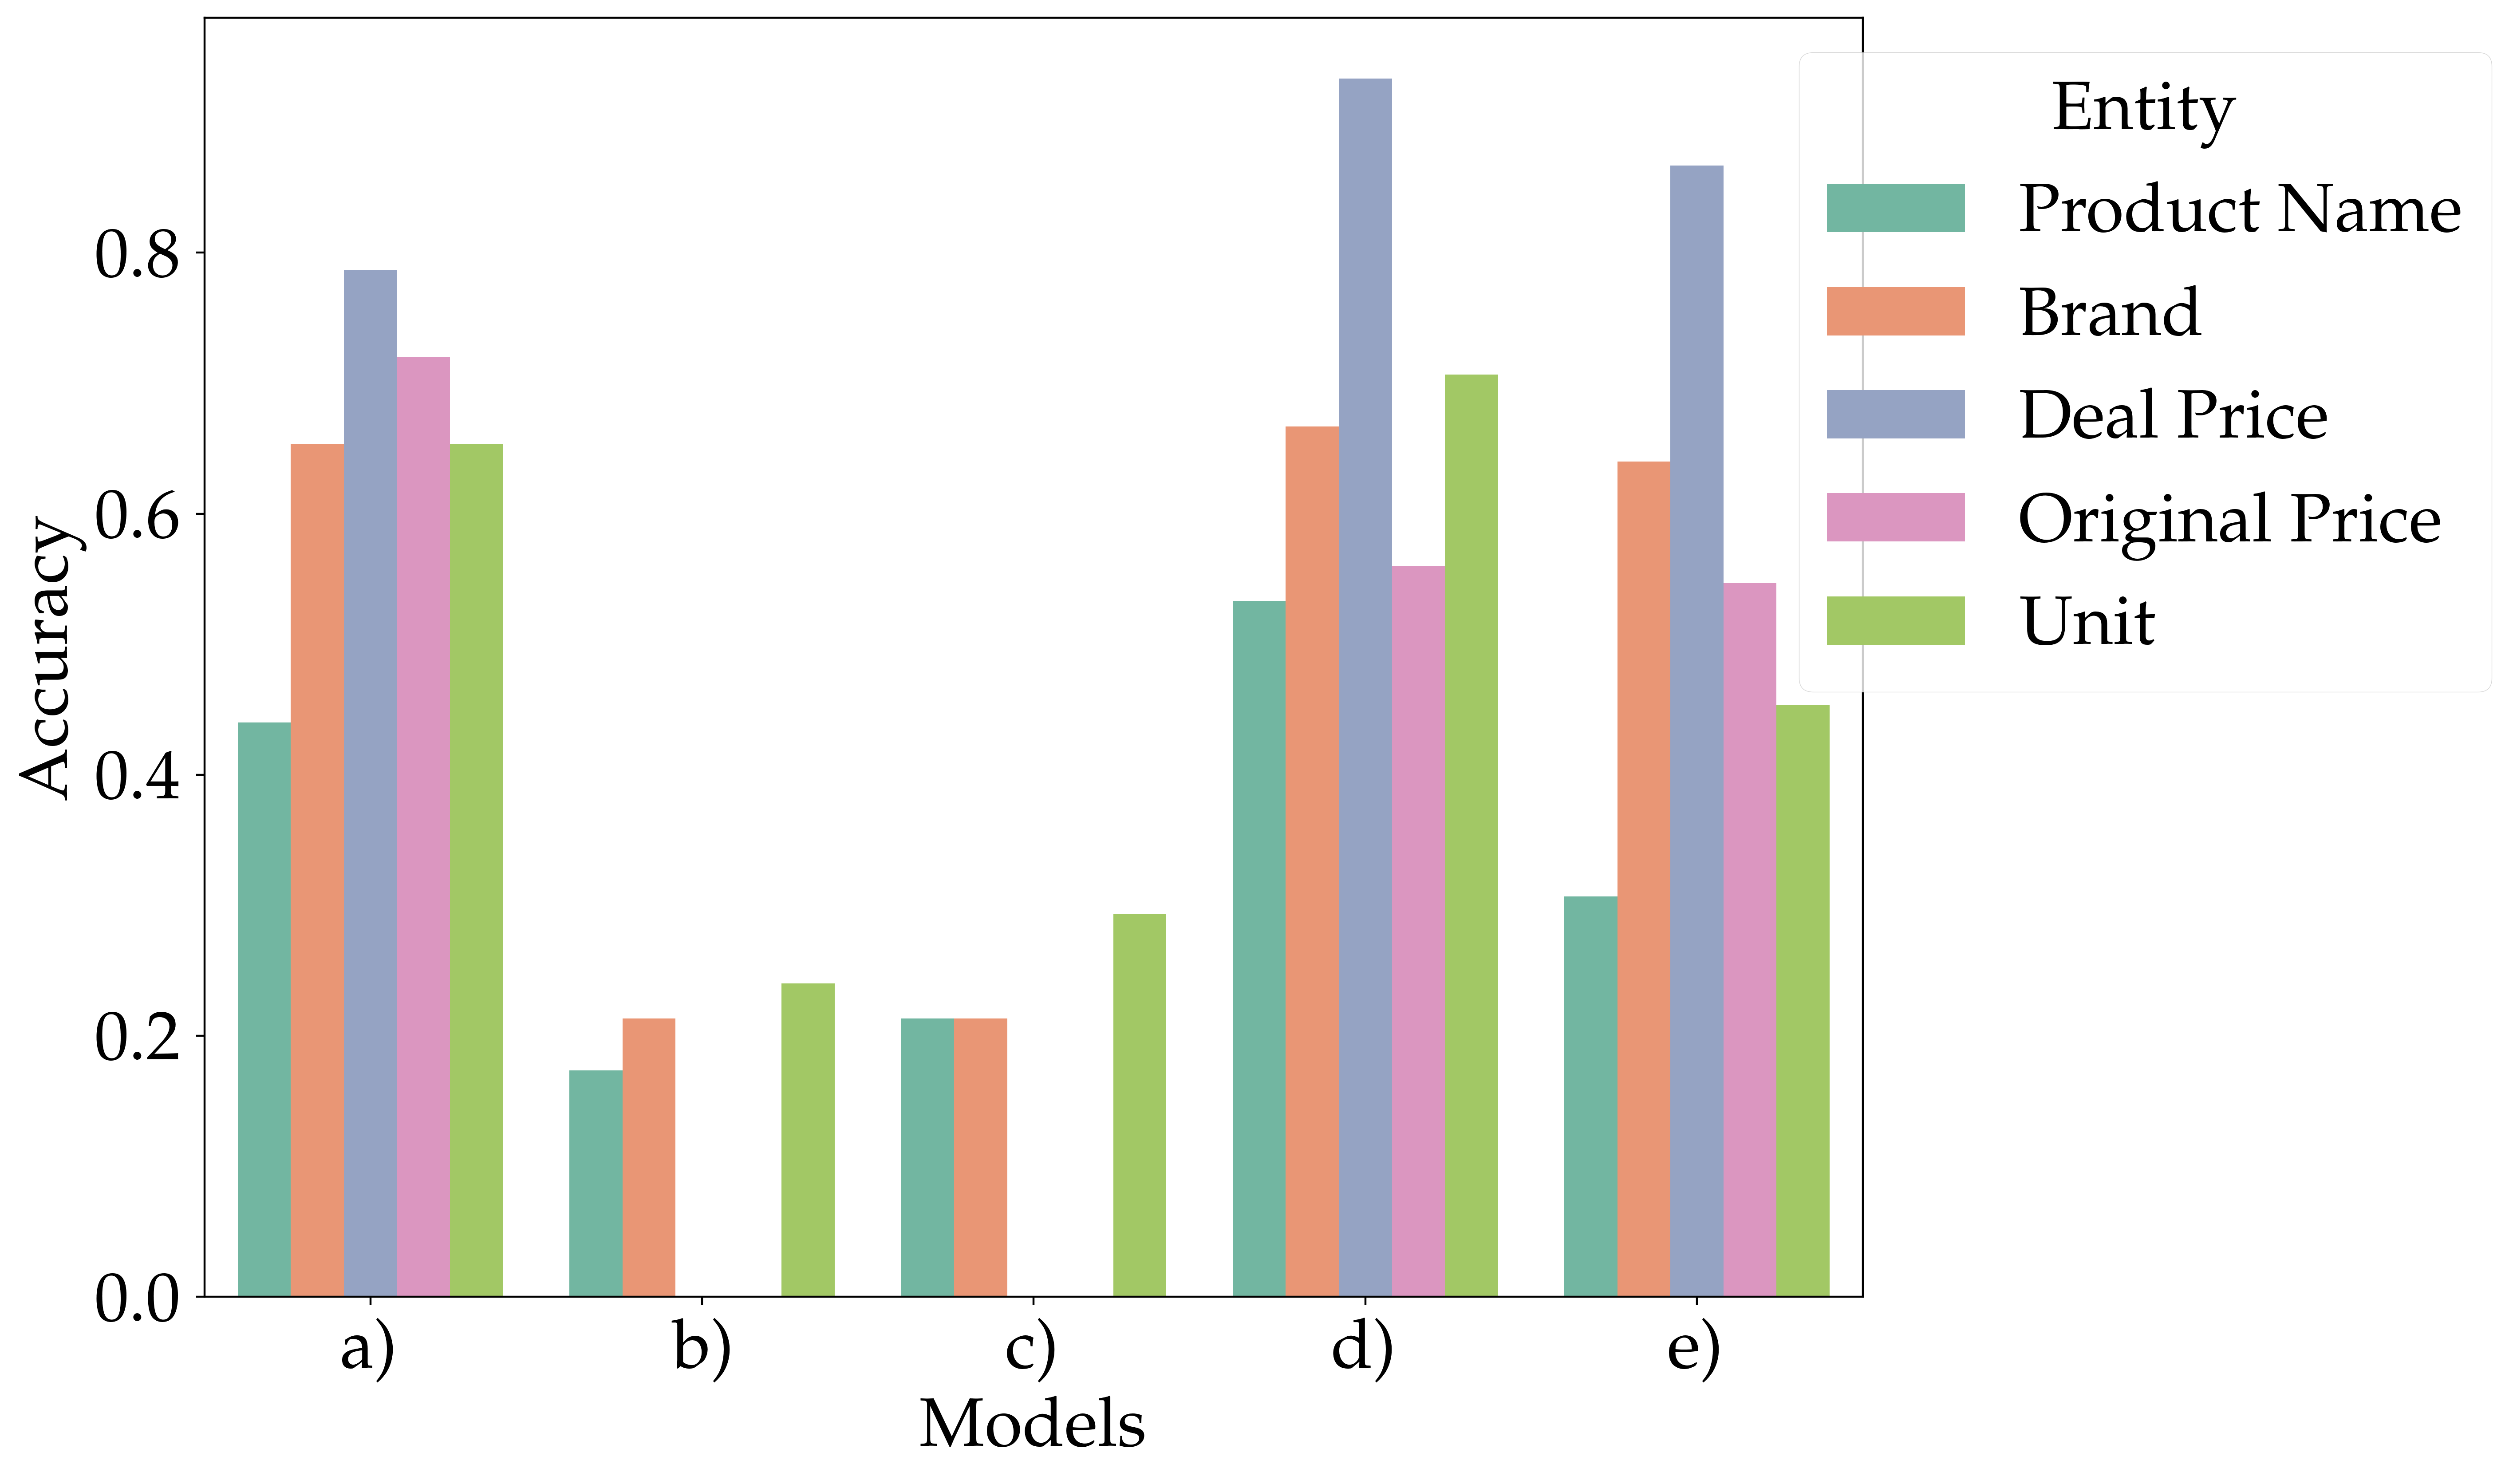
\includegraphics[width=0.8\linewidth]{figures/accuracies_raw.png}
    \caption{Per-Entity Accuracy without normalization. a: Donut, b: docTR + Qwen 2.5 [7b, Q4], c: docTR + Llama 3.1 [8b, Q4], d: MiniCPM-V, e: Llama3.2-Vision.}
    \label{fig:eval_final_acc_raw}
\end{figure*}

\begin{figure*}[h!]
    \centering
    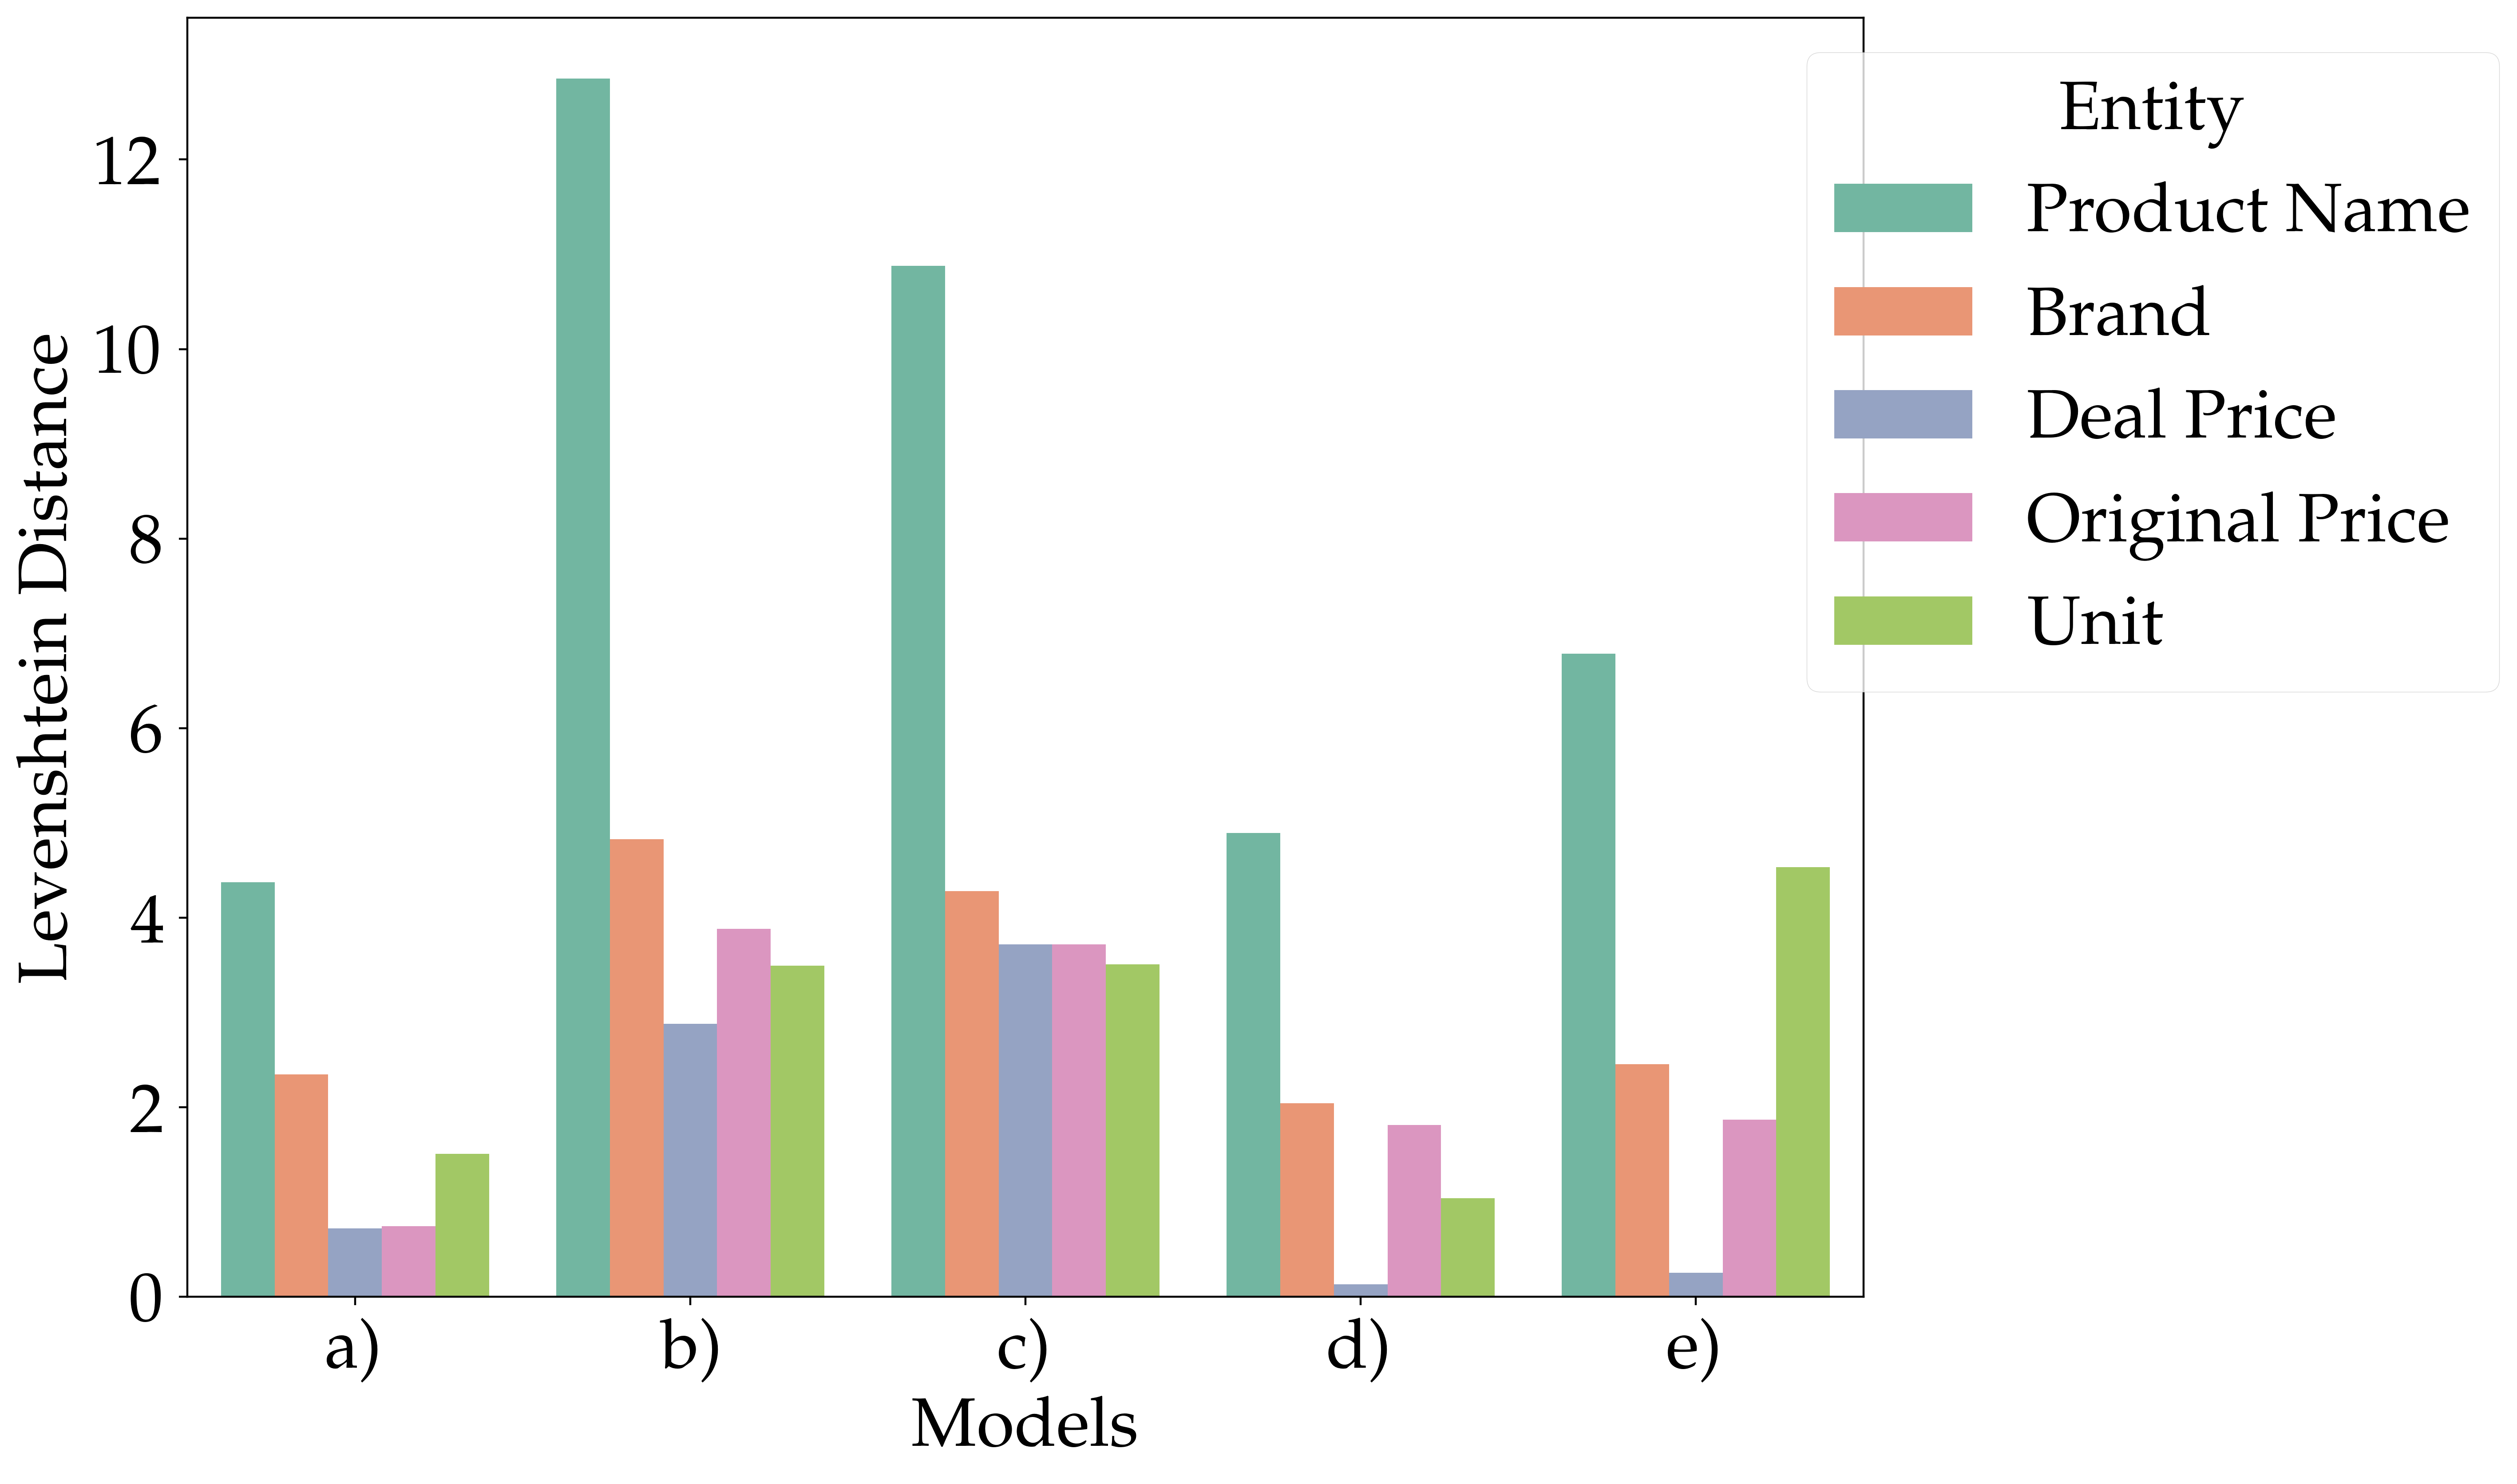
\includegraphics[width=0.8\linewidth]{figures/levdistances_raw.png}
    \caption{Per-Entity Levenshtein Distance without normalization. a: Donut, b: docTR + Qwen 2.5 [7b, Q4], c: docTR + Llama 3.1 [8b, Q4], d: MiniCPM-V, e: Llama3.2-Vision.}
    \label{fig:eval_final_levdis_raw}
\end{figure*}

Normalization significantly improved results, as shown in \figref{fig:eval_final_acc_norm} and \figref{fig:eval_final_levdis_norm}, particularly for OCR+LLM, which saw its price detection accuracy surpass Donut in some cases. However, OCR+LLM remained inferior to LVLMs and Donut overall. Donut displayed stable and balanced accuracy across entities, while LVLMs, despite higher variance, maintained their lead, excelling in price extraction. Post-normalization, Levenshtein distances decreased across all models, with OCR+LLM showing the most substantial reduction. LVLMs achieved the lowest distances but with higher variance, whereas Donut demonstrated remarkable consistency. Despite these improvements, brand names continued to exhibit the highest Levenshtein distances, highlighting the persistent challenge of accurately extracting this entity even after normalization. These results, visualized in the referenced figures, underscore the strengths of LVLMs in leveraging multimodal cues and the robustness of Donut, while revealing the limitations of OCR+LLM pipelines in handling complex, noisy leaflet data.

\begin{figure*}[h!]
    \centering
    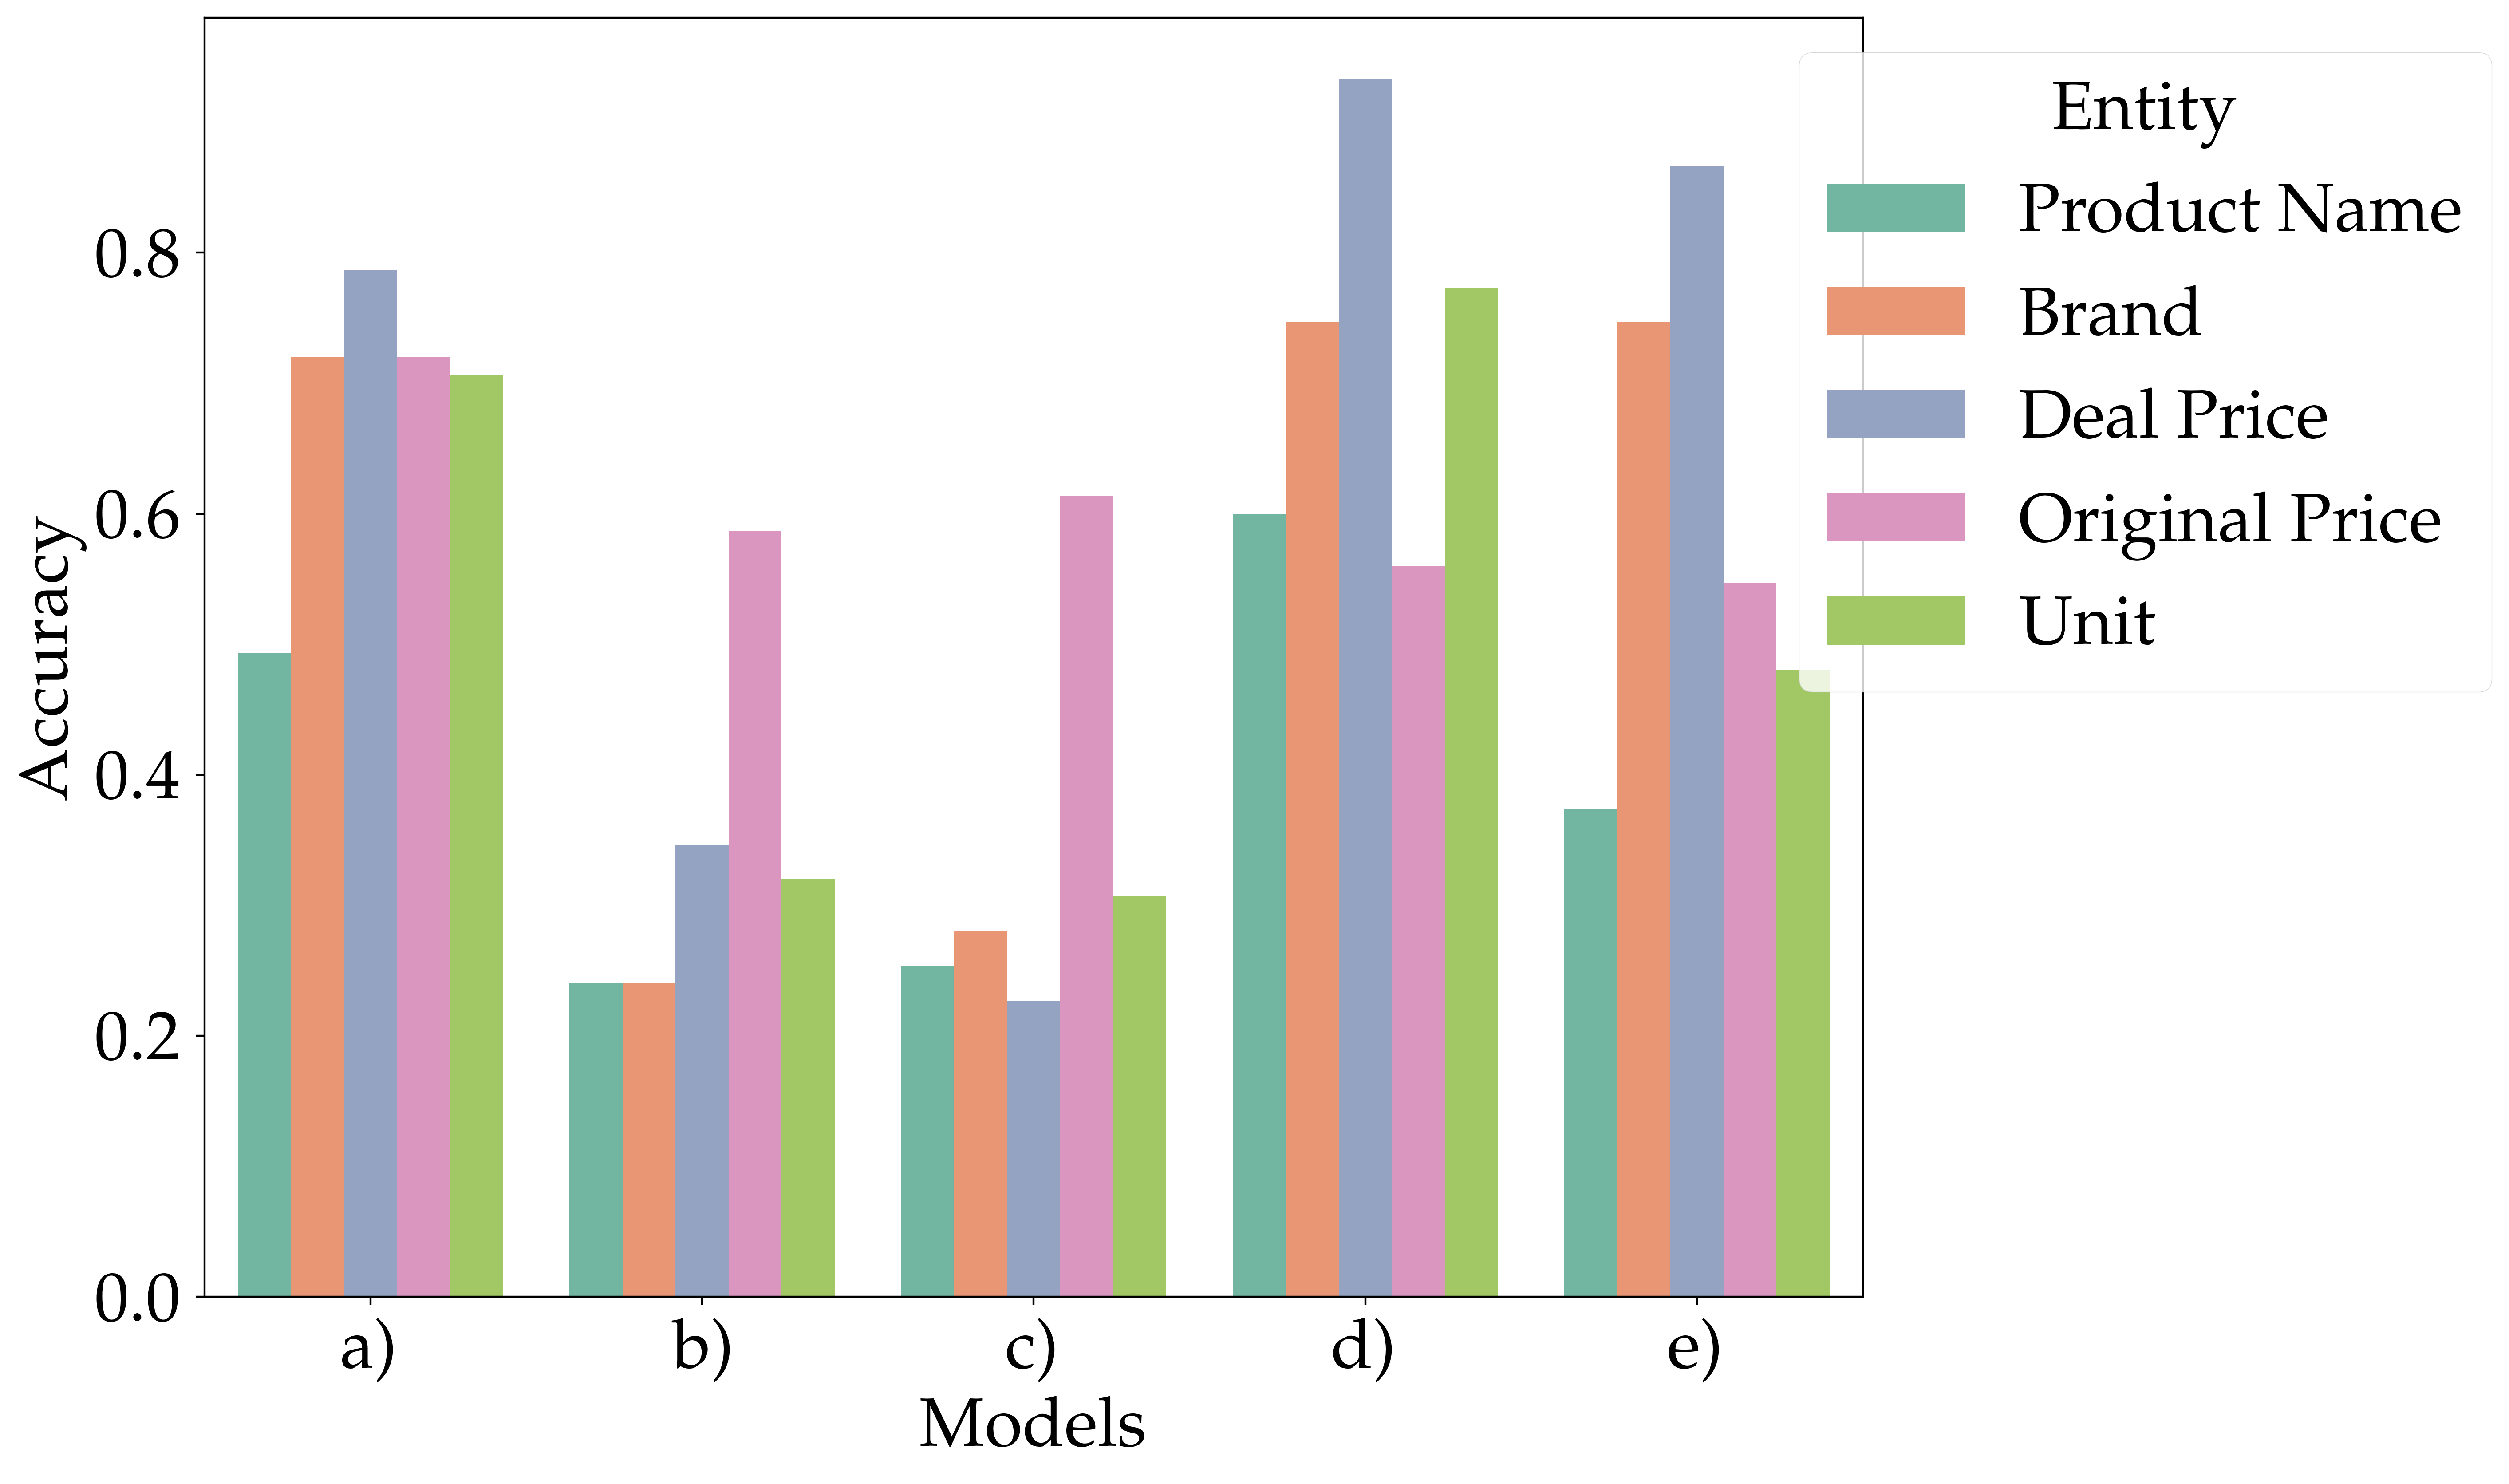
\includegraphics[width=0.8\linewidth]{figures/accuracies_norm.png}
    \caption{Per-Entity Accuracy with normalization. a: Donut, b: docTR + Qwen 2.5 [7b, Q4], c: docTR + Llama 3.1 [8b, Q4], d: MiniCPM-V, e: Llama3.2-Vision.}
    \label{fig:eval_final_acc_norm}
\end{figure*}

\begin{figure*}[h!]
    \centering
    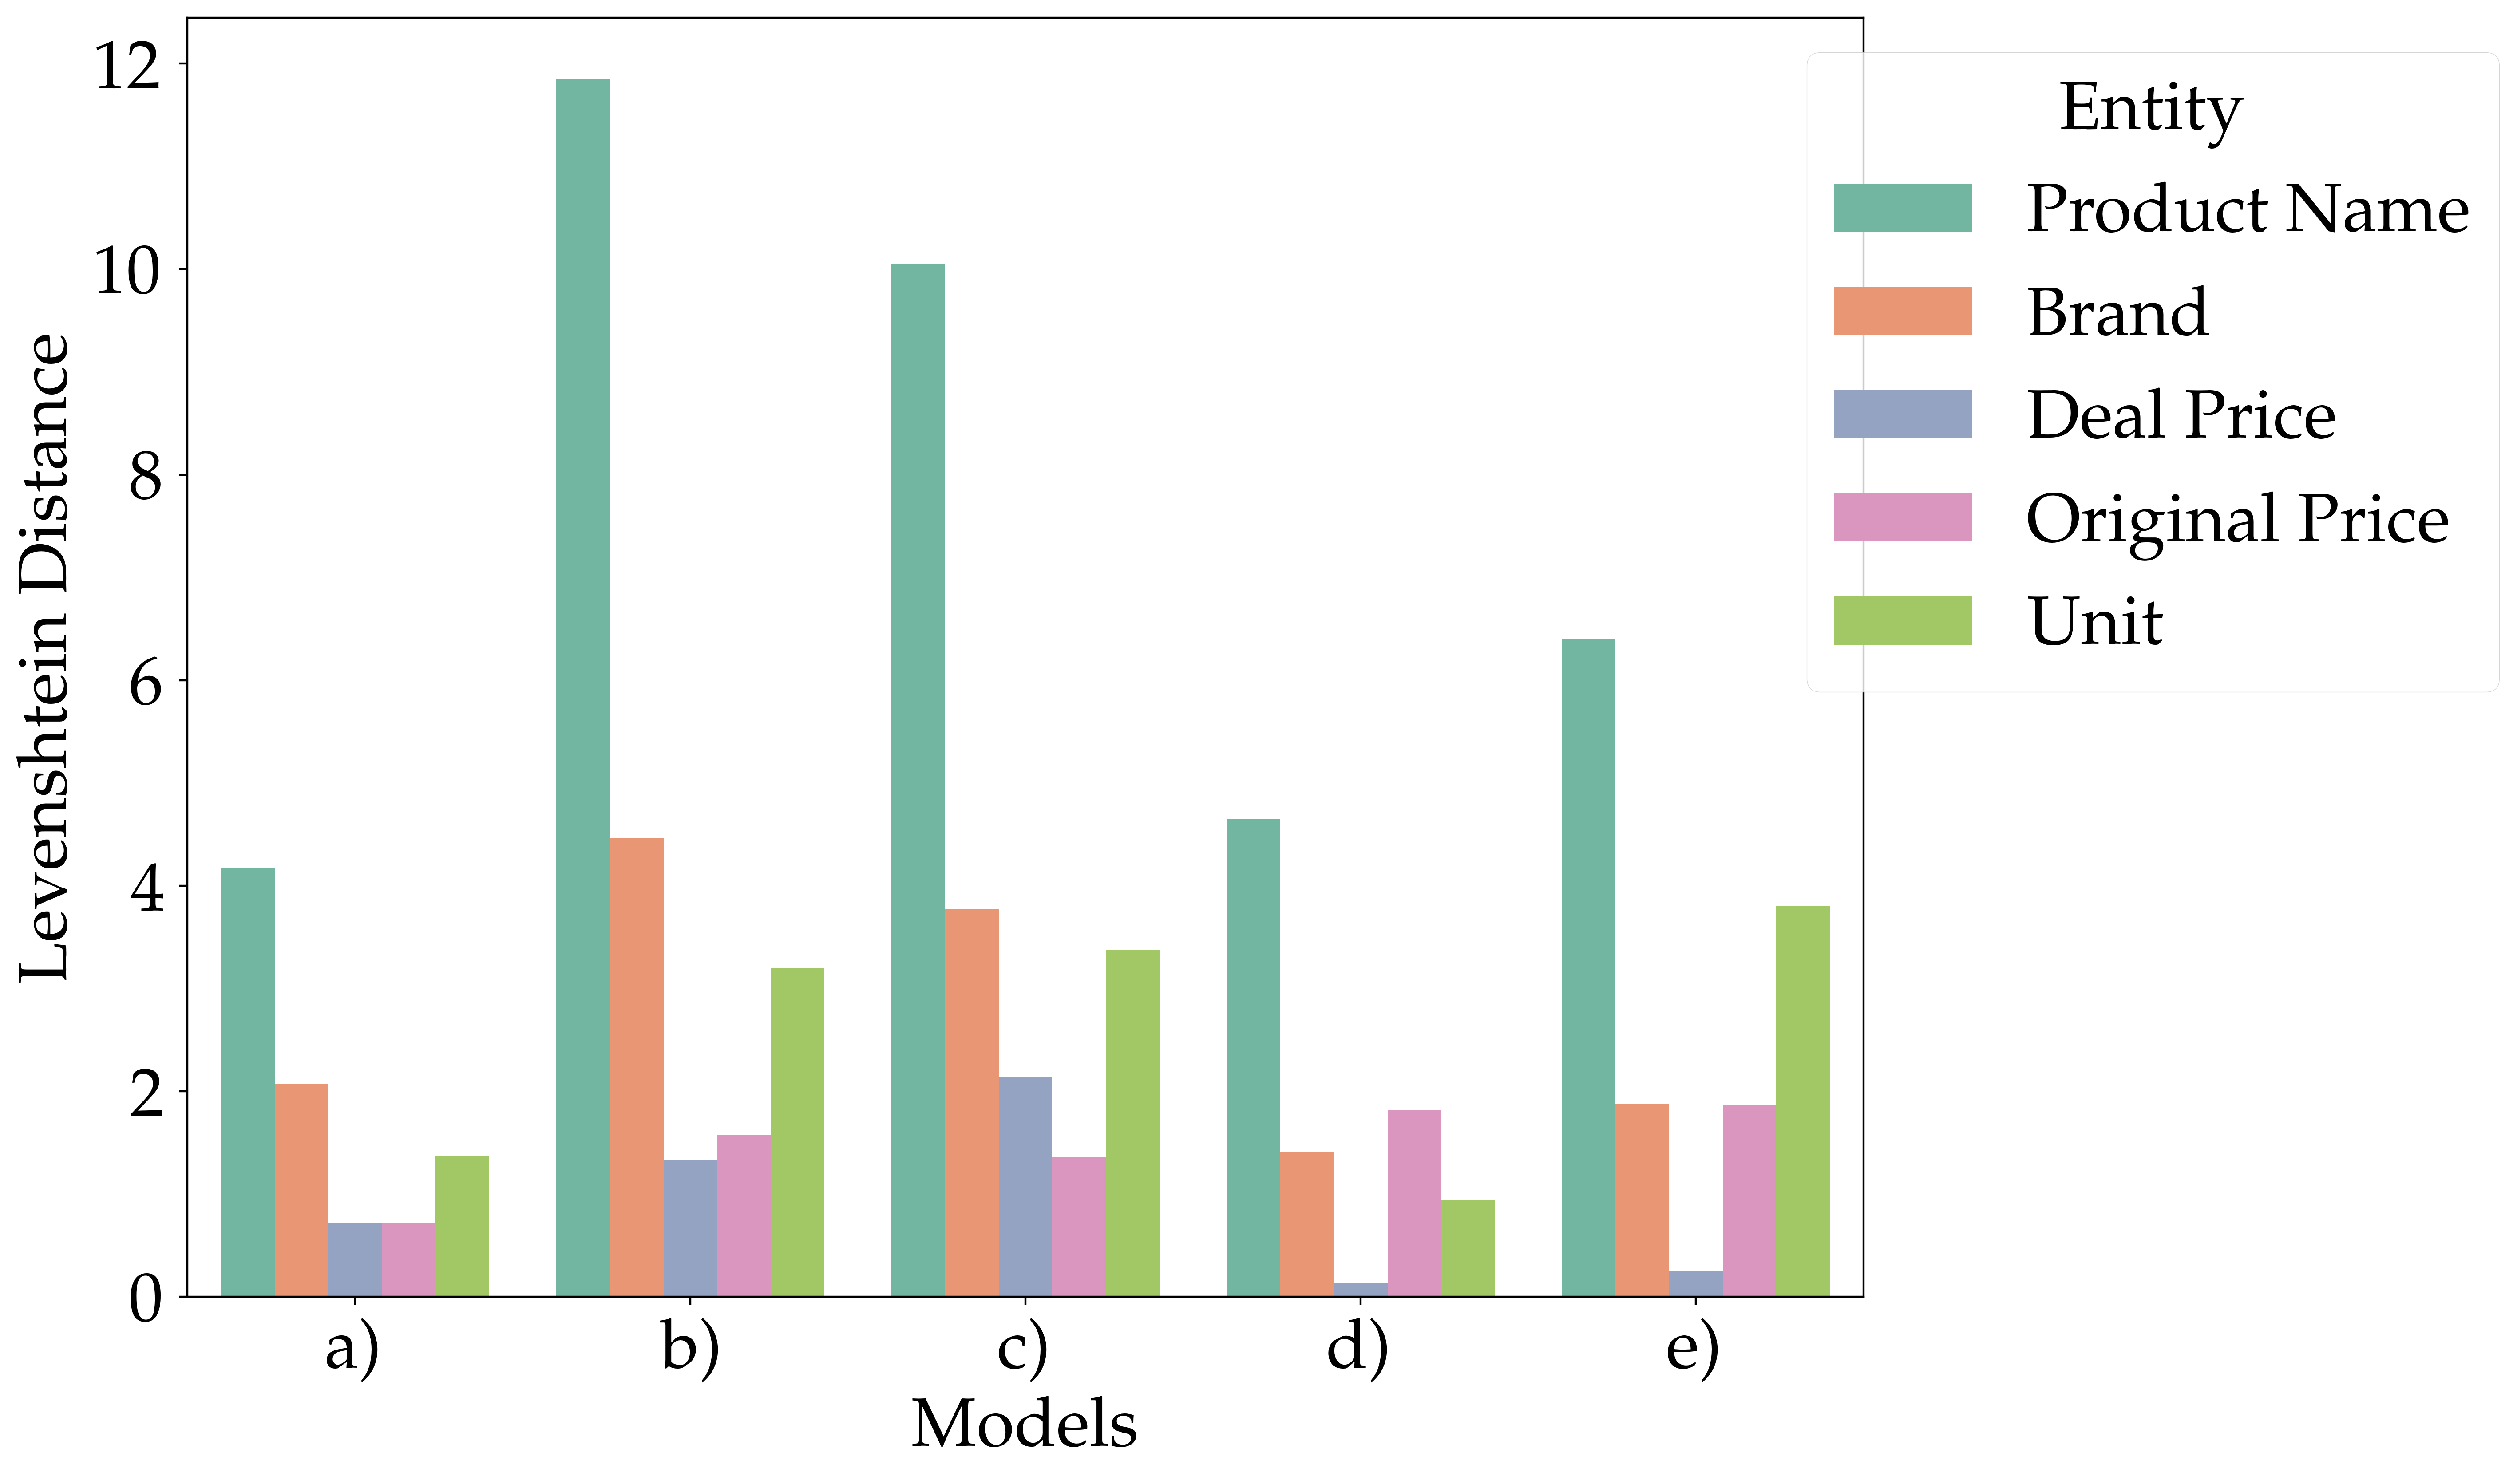
\includegraphics[width=0.8\linewidth]{figures/levdistances_norm.png}
    \caption{Per-Entity Levenshtein Distance with normalization. a: Donut, b: docTR + Qwen 2.5 [7b, Q4], c: docTR + Llama 3.1 [8b, Q4], d: MiniCPM-V, e: Llama3.2-Vision.}
    \label{fig:eval_final_levdis_norm}
\end{figure*}

\indent{\textbf{Dicussion.}} The evaluation highlights distinct strengths and limitations across the tested models. LVLMs emerged as the most effective for IE tasks, particularly when spatial and visual context is critical. However, their superior performance comes at the cost of significantly higher computational requirements, making them less practical for resource-constrained environments. Donut offers a compelling trade-off between accuracy and efficiency, demonstrating strong performance despite limited training resources. With further optimization, Donut has the potential to surpass LVLMs for this specific task, though its generalization ability remains narrower compared to LVLMs, which excel across a broader range of tasks.

In contrast, the OCR+LLM pipeline proved considerably weaker than both LVLMs and Donut. This performance gap stems from several factors: (1) the lack of spatial and visual information, which limits its ability to resolve ambiguities; (2) error propagation from the OCR stage to the LLM, compounding inaccuracies; and (3) insufficient training data to achieve robust IE performance. Despite these limitations, OCR+LLM remains a viable option for scenarios with constrained computational resources and moderate task complexity, where its simplicity and lower resource demands may outweigh its performance drawbacks.


\section{Application}
\label{sec:application}
The ability to detect deals from a wide range of supermarket leaflets provides the foundation for extracting structured information and building a centralized deal database. If all components, from deal detection to information extraction, function reliably, this enables the creation of a comprehensive repository containing deals from various supermarkets, based solely on the content of their weekly unstructured leaflets. Such a structured database allows for numerous applications, including price trend analysis, intelligent shopping list generation and deal comparison across stores. The immediate objective of this project was to develop a system that could automatically collect, process and present extracted deals in a structured manner. The resulting application is designed to scrape supermarket leaflets weekly, detect deals using the trained YOLO-based model and extract relevant metadata, including product names and prices. These extracted deals are then stored in a structured format within a database and made accessible through a web-based interface.

\subsection{Database}
\begin{figure*}[h!]
    \centering
    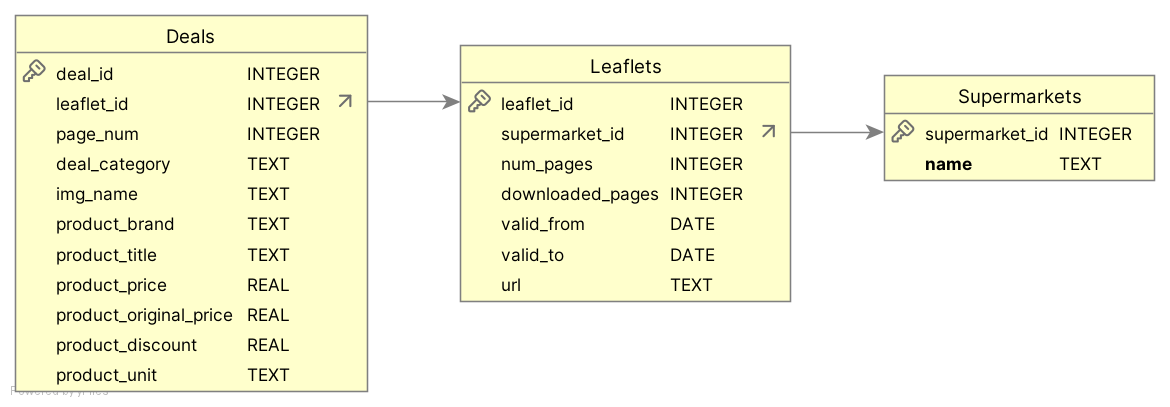
\includegraphics[width=0.8\linewidth]{figures/application/db_uml.png}
    \caption{Database schema for storing metadata for supermarket leaflets and extracted deals.}
    \label{fig:application_db_uml}
\end{figure*}
For storing the extracted deals, a lightweight and efficient solution was required. SQLite was chosen due to its simplicity and fast performance, making it well-suited for handling the structured but relatively small-scale dataset. After several weeks of scraping supermarket leaflets, the dataset grew to include 540 leaflets from 20 different supermarkets. The database is structured into three primary tables (cf. Figure \ref{fig:application_db_uml}): one for supermarket metadata, one for storing the leaflets and one containing the extracted deals. The total number of extracted deals in the database adds up to 47,829. Among these, the vast majority (46,869) are classified as standard deals, while 607 fall under product category deals, 144 correspond to coupons and 208 belong to miscellaneous categories. Since the structure and content of non-standard deals often differ significantly from regular deals featuring loyalty points, bulk discounts, or percentage-based reductions across entire product groups, the primary focus remains on standard deals. By structuring the data efficiently, the database serves as a robust backend for the subsequent web application, facilitating fast queries and scalable deal retrieval.

\subsection{Web User Interface}
\begin{figure*}[h!]
    \centering
    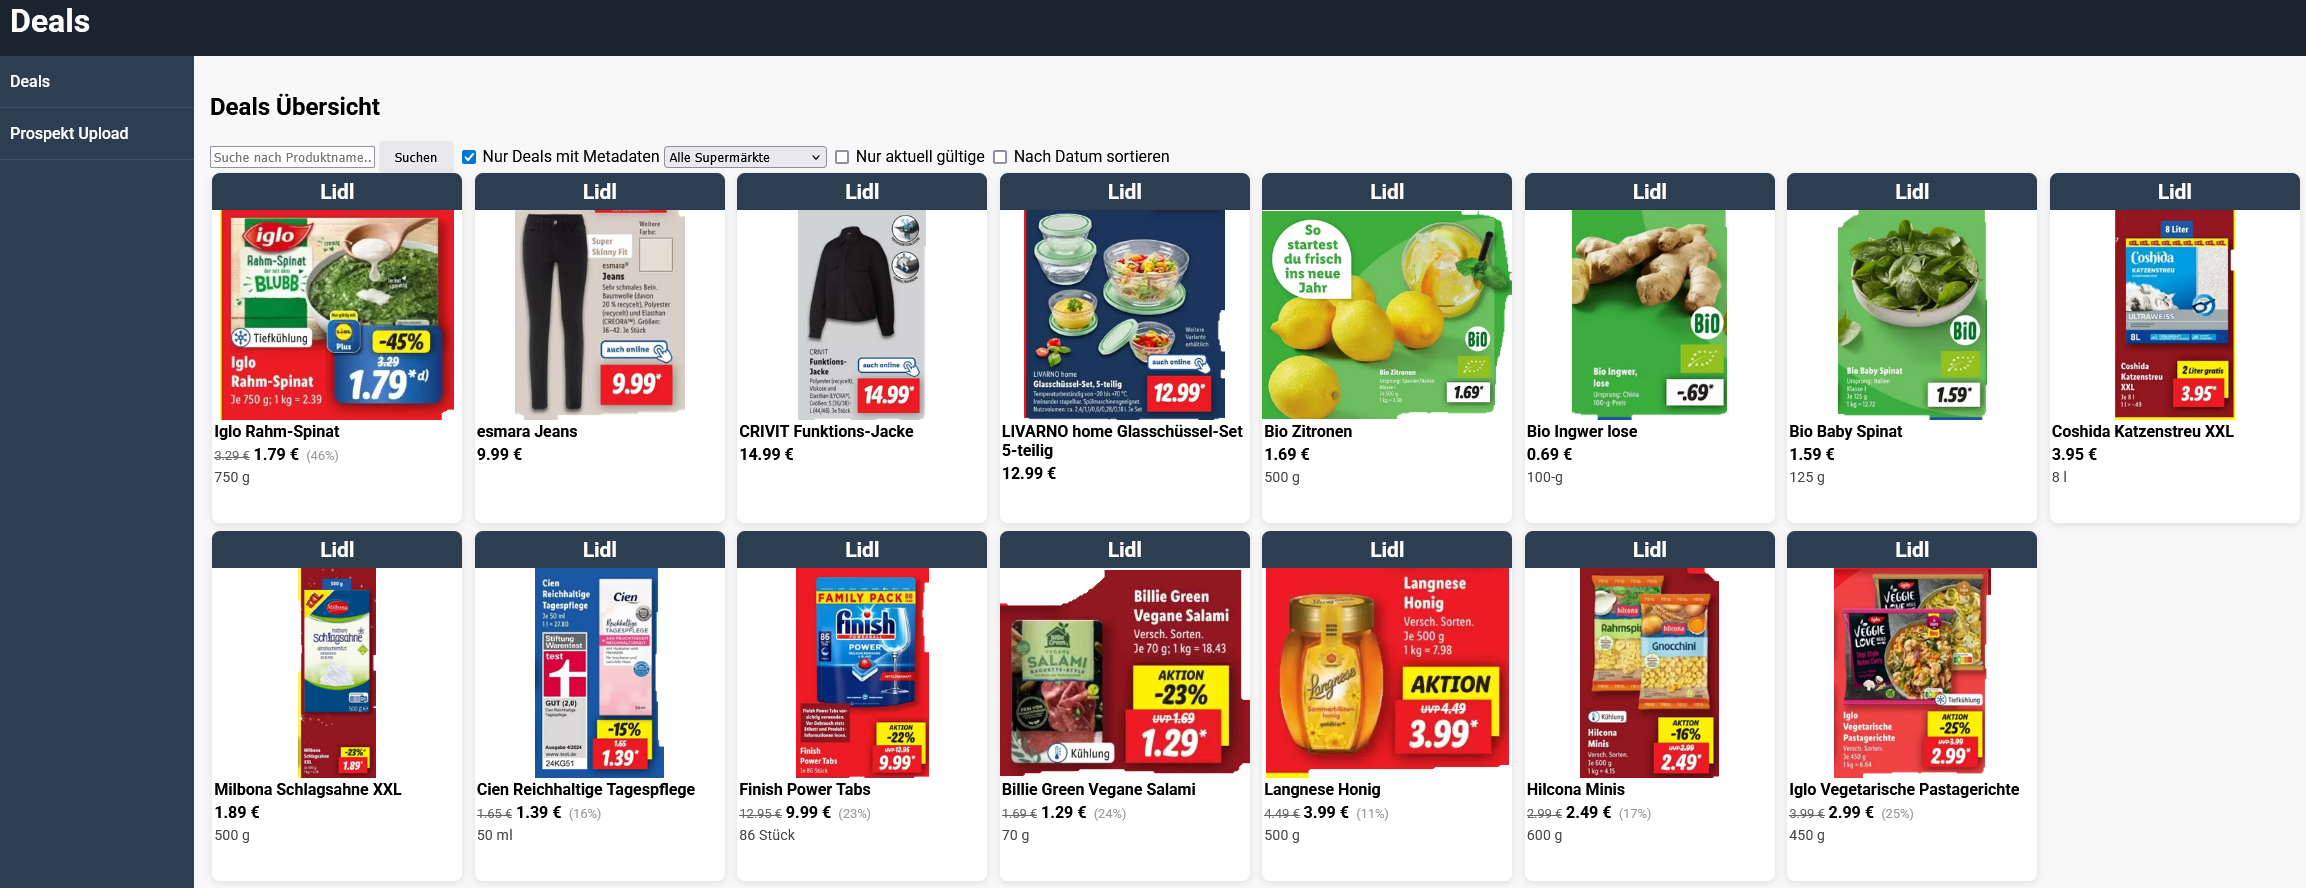
\includegraphics[width=0.8\linewidth]{figures/application/deals_overview.png}
    \caption{Web-based application interface for browsing all extracted supermarket deals with search and filter functionality.}
    \label{fig:application_web_overview}
\end{figure*}

Building on the database, a web-based application was developed to provide users with an interactive way to explore supermarket deals, which is shown in Figure \ref{fig:application_web_overview}. The core functionality centers around an intuitive search system that allows users to find deals based on specific product names. Additionally the interface supports filtering options, enabling users to refine searches by supermarket chain or deal validity period. Each deal is displayed with its corresponding image snippet, extracted metadata, and pricing information, making it easy to compare offers across different retailers.

\begin{figure*}[h!]
    \centering
    \begin{tabular}{cc}
    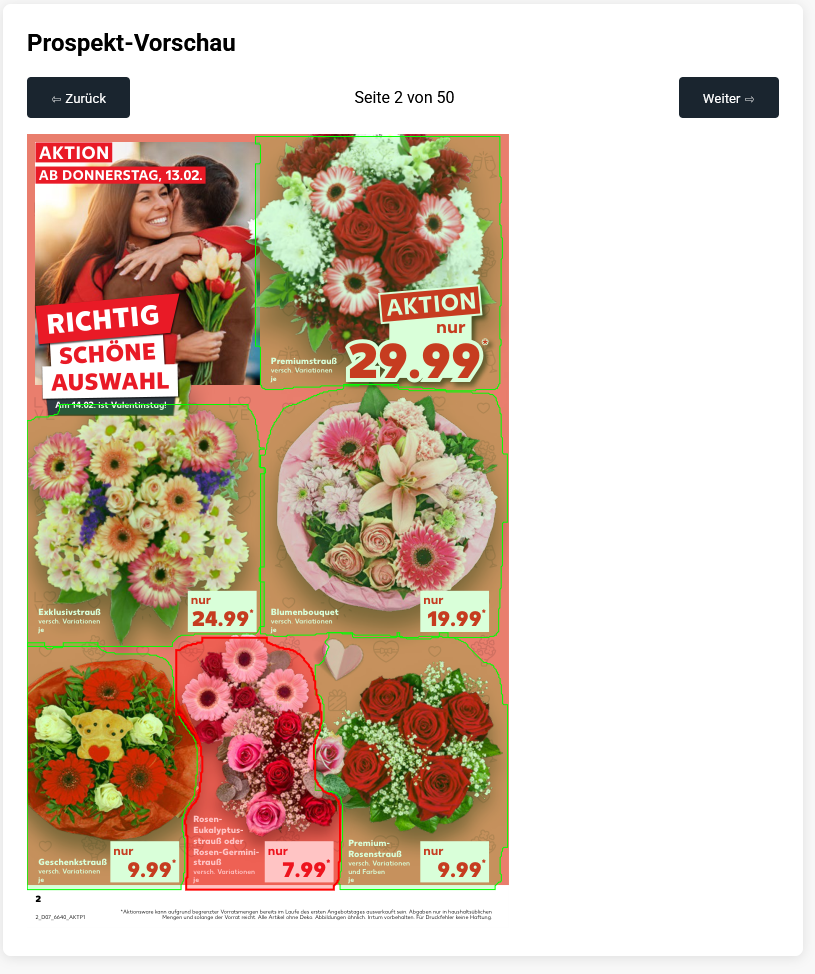
\includegraphics[width=0.45\linewidth]{figures/application/leaflet_segmentations.png} &   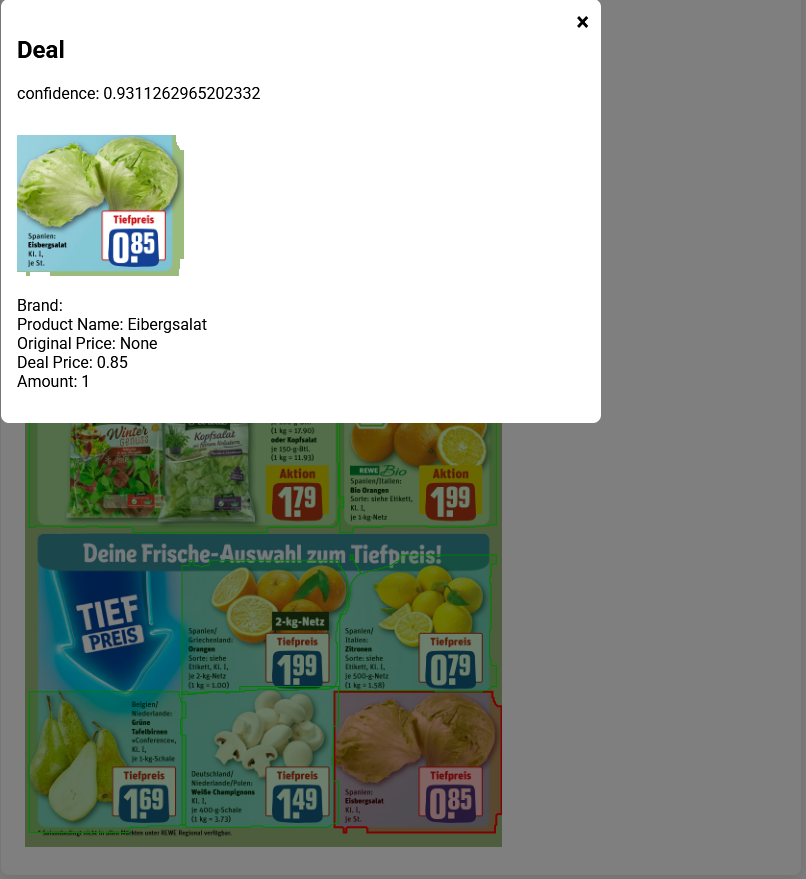
\includegraphics[width=0.45\linewidth]{figures/application/single_deal.png} \\
    (a) Interactive leaflet segmentation & (b) Detailed view of a single deal \\[2pt]
    \end{tabular}
    \caption{Additional features of the web application, including interactive uploading of pdf leaflets and detailed deal views by clicking on individual deals.}
    \label{fig:application_combined}
\end{figure*}

Beyond static deal browsing, the application also incorporates an upload feature that enables users to submit entire supermarket leaflets for processing. When a leaflet is uploaded, the system applies the full processing pipeline, from deal detection using YOLO to information extraction. The processed leaflet can then be browsed interactively, displaying detected deals with their segmentation masks overlaid on the original pages. This feature provides direct insights into the models performance, allowing users to verify the accuracy of detected promotions and extracted information. The efficiency of the application benefits from  lightweight architecture from YOLO, ensuring that leaflet processing remains fast and responsive. After a short processing time, users can navigate through detected deals and inspect the segmentation masks applied to the leaflet images. Clicking on an individual deal reveals extracted details such as the product name, price, and other metadata. The combination of automated deal extraction and interactive visualization makes the web application a practical tool for structured deal exploration and comparison.

\section{Conclusion}
\label{sec:conclusion}
    \subsection{Summary}
    This work presents a comprehensive approach to the digitalization and structuring of supermarket leaflet deals. The proposed modular pipeline encompasses deal detection and information extraction, transforming raw leaflet data into structured data. The deal detection module leverages lightweight and efficient YOLO-based models to accurately identify and segment deals within leaflets, while the information extraction module employs state-of-the-art OCR, LLM, and end-to-end models to extract and normalize deal attributes. The developed interactive application, backed by a robust database, allows users to browse, filter, and compare deals across multiple supermarket chains, providing a proof of concept for practical applications. Additionally, the research contributes two datasets: one for deal detection as instance segmentation and another for image-based information extraction, facilitating further research in this domain.

    \subsection{Future Work}
    This project opens up several avenues for future research and development to enhance the system's capabilities and usability.

    Firstly, enhancing the performance and runtime of the deal detection module is crucial. This involves optimizing the existing YOLO-based model and exploring alternative architectures that may offer better accuracy and efficiency. Also, the size of the dataset can be increased by including more leaflets from different supermarkets, which would improve the model's generalization capabilities.

    Secondly, the IE component can be significantly improved by building a larger dataset specifically for training the Donut model. Given the promising results achieved with Donut, expanding the dataset and fine-tuning the model further could yield competitive results in extracting structured information from supermarket leaflets.

    Additionally, several new branches of research and development can be pursued. These include the deal specification and product image extraction to build a comprehensive database, brand and product name normalization for database mapping, and time series analysis for price trend prediction. On the application side, scalability, frontend improvements, and additional features such as a recommendation engine and automatic weekly deal extraction can enhance user experience and system robustness. There are numerous possibilities for future work and the project serves as a foundation for further exploration in the field of supermarket deal extraction based on leaflets.

\bibliography{references}
\newpage

\appendix
\section*{Appendices}
\numberwithin{figure}{section}
\numberwithin{table}{section}
\addcontentsline{toc}{section}{Appendices}
\renewcommand{\thesubsection}{\Alph{subsection}}

\subsection{OCR Evaluation: Normalization Procedure}
\label{app:ocr_normalization}
The procedure is implemented as a multi-level function, where each level applies increasingly rigorous transformations. Below, we provide a detailed explanation of the normalization steps and present the procedure in pseudocode.

\begin{algorithm}[H]
\caption{Text Normalization Function}
\label{alg:normalization}
\begin{algorithmic}[1]
\Require Input text $text$, normalization level $level$ (default: 6)
\Ensure Normalized text
\State \textbf{Initialize}: If $text$ is empty, null, or an empty string, return an empty string.
\If{$level \geq 1$}
    \State Strip leading and trailing whitespace from $text$.
\EndIf
\If{$level \geq 2$}
    \State Convert $text$ to lowercase.
    \State Replace newline, tab, and carriage return characters with spaces.
    \State Normalize German characters: "ö" $\rightarrow$ "o", "ä" $\rightarrow$ "a", "ü" $\rightarrow$ "u", "ß" $\rightarrow$ "ss".
\EndIf
\If{$level \geq 3$}
    \State Replace hyphens and dashes  with spaces.
    \State Remove all non-alphanumeric characters except periods and spaces.
    \State Collapse multiple spaces into a single space.
\EndIf
\If{$level \geq 4$}
    \State Remove all spaces and periods from $text$.
\EndIf
\State \textbf{Return} normalized $text$.
\end{algorithmic}
\end{algorithm}

The normalization function is applied to both OCR outputs and ground truth texts before evaluation. By standardizing the text at various levels, we ensure that the evaluation metrics are robust to minor formatting differences and focus on the semantic accuracy of the OCR system.

\subsection{LLM Prompt for Structured Information Extraction}
\label{app:llm_prompt}

This appendix details the prompt template used to guide the Large Language Model (LLM) in extracting structured information from OCR text. The prompt is designed to ensure consistent and accurate extraction of supermarket deal information, including fields such as brand name, product name, original price, reduced price, and weight. Below, we provide the system template, instructions, and an example of the prompt in action.

The system template defines the context, extraction requirements, and instructions for the LLM. It is structured as follows:


\begin{verbatim}
**Context:**  
You are an advanced language model specializing in extracting 
structured information from OCR text. 
Your task is to extract one supermarket deal from the given OCR result.

**Extraction Requirements:**  
- **Fields:**  
  - "Marke": Brand name (if explicitly mentioned)  
  - "Produktname": Product name  
  - "Original Preis": Original price  
  - "Reduzierter Preis": Reduced price  
  - "Gewicht": Weight (if available; otherwise, use null)

- **Instructions:**  
  - Return a single JSON object containing exactly one deal.
  - Use JSON only—no additional text.
  - If a field is missing, assign a null value.
  - Correct OCR errors such as missing decimals (e.g., "229" → "2.29"), 
    incorrect spellings, and OCR noise.
  - Use contextual cues (e.g., euro symbols) to infer and correct pricing.

**Example:**  
OCR Input:                     
Dallmayr Prodomo Kaffee gemahlen 500g 1kg=51.73 Dallmayr -24% prodomo 5 69 UVP7,49  

JSON OUTPUT:
{
    "Marke": "Dallmayr",
    "Produktname": "Prodomo Kaffee gemahlen",
    "Original Preis": "UVP7,49",
    "Reduzierter Preis": "3,99 €",
    "Gewicht": null
}

IMPORTANT: Return the JSON object in the above format only once.
\end{verbatim}

The prompt is constructed by combining the system template with the OCR input provided by the user. The structure of the prompt is as follows:

\begin{verbatim}
messages = [
    SYSTEM_TEMPLATE,
    {
        "role": "user",
        "content": f"OCR Input: {ocr_res}\nJSON OUTPUT:"
    }
]
\end{verbatim}

Here, \texttt{ocr\_res} represents the OCR output text, which is dynamically inserted into the prompt.

\subsection{OCR + LLM Evaluation: Normalization Procedure}
\label{app:ocr_llm_normalization}

This appendix describes the normalization procedure applied to LLM-extracted data during evaluation. The normalization process ensures consistency by standardizing text formats, removing special characters, and correcting common OCR errors. Below, we provide a detailed explanation of the procedure and present the implementation in pseudocode.

The normalization procedure is implemented as a Python function that performs the following steps:

\begin{algorithm}[H]
\caption{Text Normalization Procedure}
\label{alg:final_normalization}
\begin{algorithmic}[1]
\Require Input text $text$
\Ensure Normalized text
\State \textbf{Initialize}: Define a dictionary $REPLACEMENTS$ for character replacements.
\State $REPLACEMENTS \gets \{
    \text{"ä"} \rightarrow \text{"a"}, \text{"ö"} \rightarrow \text{"o"}, \text{"ü"} \rightarrow \text{"u"}, 
    \text{"ß"} \rightarrow \text{"ss"}, \text{","} \rightarrow \text{"."}, \text{"€"} \rightarrow \text{""}, 
    \text{"ô"} \rightarrow \text{"o"}, \text{"é"} \rightarrow \text{"e"}, \text{"ç"} \rightarrow \text{"c"}, 
    \text{"è"} \rightarrow \text{"e"}, \text{"à"} \rightarrow \text{"a"}, \text{"ê"} \rightarrow \text{"e"}, 
    \text{"â"} \rightarrow \text{"a"}, \text{"û"} \rightarrow \text{"u"}, \text{"î"} \rightarrow \text{"i"}, 
    \text{"ë"} \rightarrow \text{"e"}, \text{"ï"} \rightarrow \text{"i"}, \text{"œ"} \rightarrow \text{"oe"}, 
    \text{"æ"} \rightarrow \text{"ae"}, \text{"ù"} \rightarrow \text{"u"}
\}$
\For{each $(key, value)$ in $REPLACEMENTS$}
    \State Replace occurrences of $key$ with $value$ in $text$.
\EndFor
\State Filter $text$ to retain only alphanumeric characters, periods, and spaces.
\State Remove all whitespace from $text$.
\State Convert $text$ to lowercase.
\State \textbf{Return} normalized $text$.
\end{algorithmic}
\end{algorithm}


\subsection{OCR + LLM Evaluation: Entity-specific results per OCR model}
\label{app:ocr_llm_results}

This section collects further detailed results for the OCR + LLM evaluation for interested readers. The results are presented in the form of per-entity accuracies and Levenshtein distances for each OCR model used in the evaluation. The figures provide insights into the performance of each OCR model in extracting structured information from supermarket leaflets, highlighting the strengths and weaknesses of individual models across different entities.

\begin{figure*}[h!]
    \begin{tabular}{cc}
      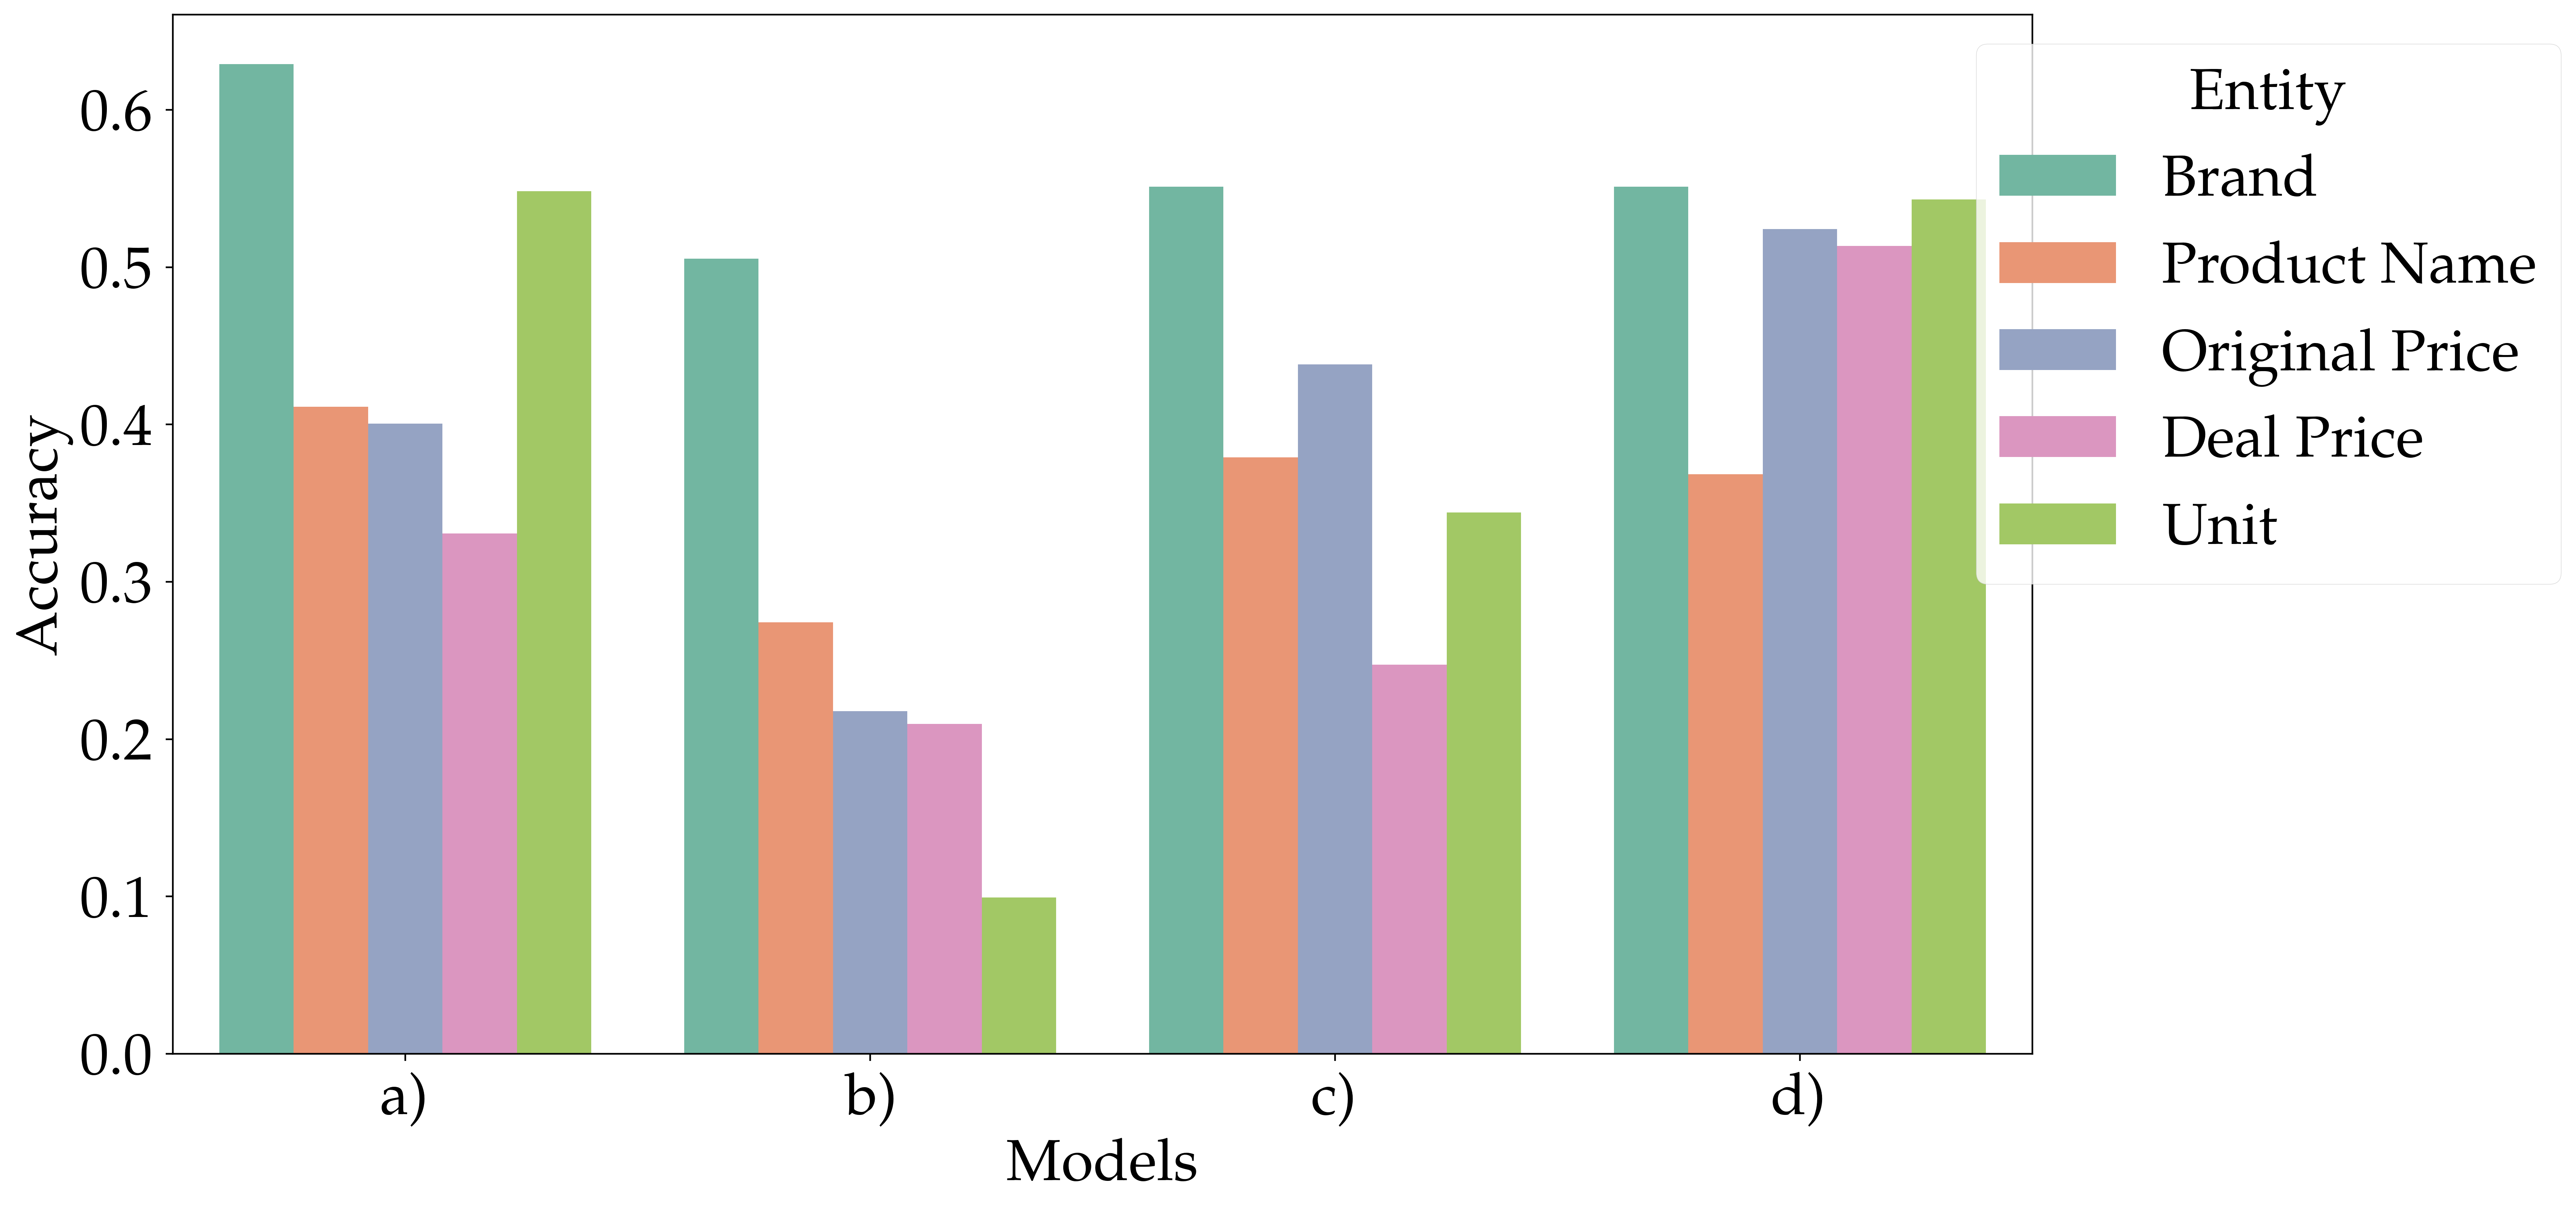
\includegraphics[width=0.5\linewidth]{figures/doctr_ocr_accuracies.png} &   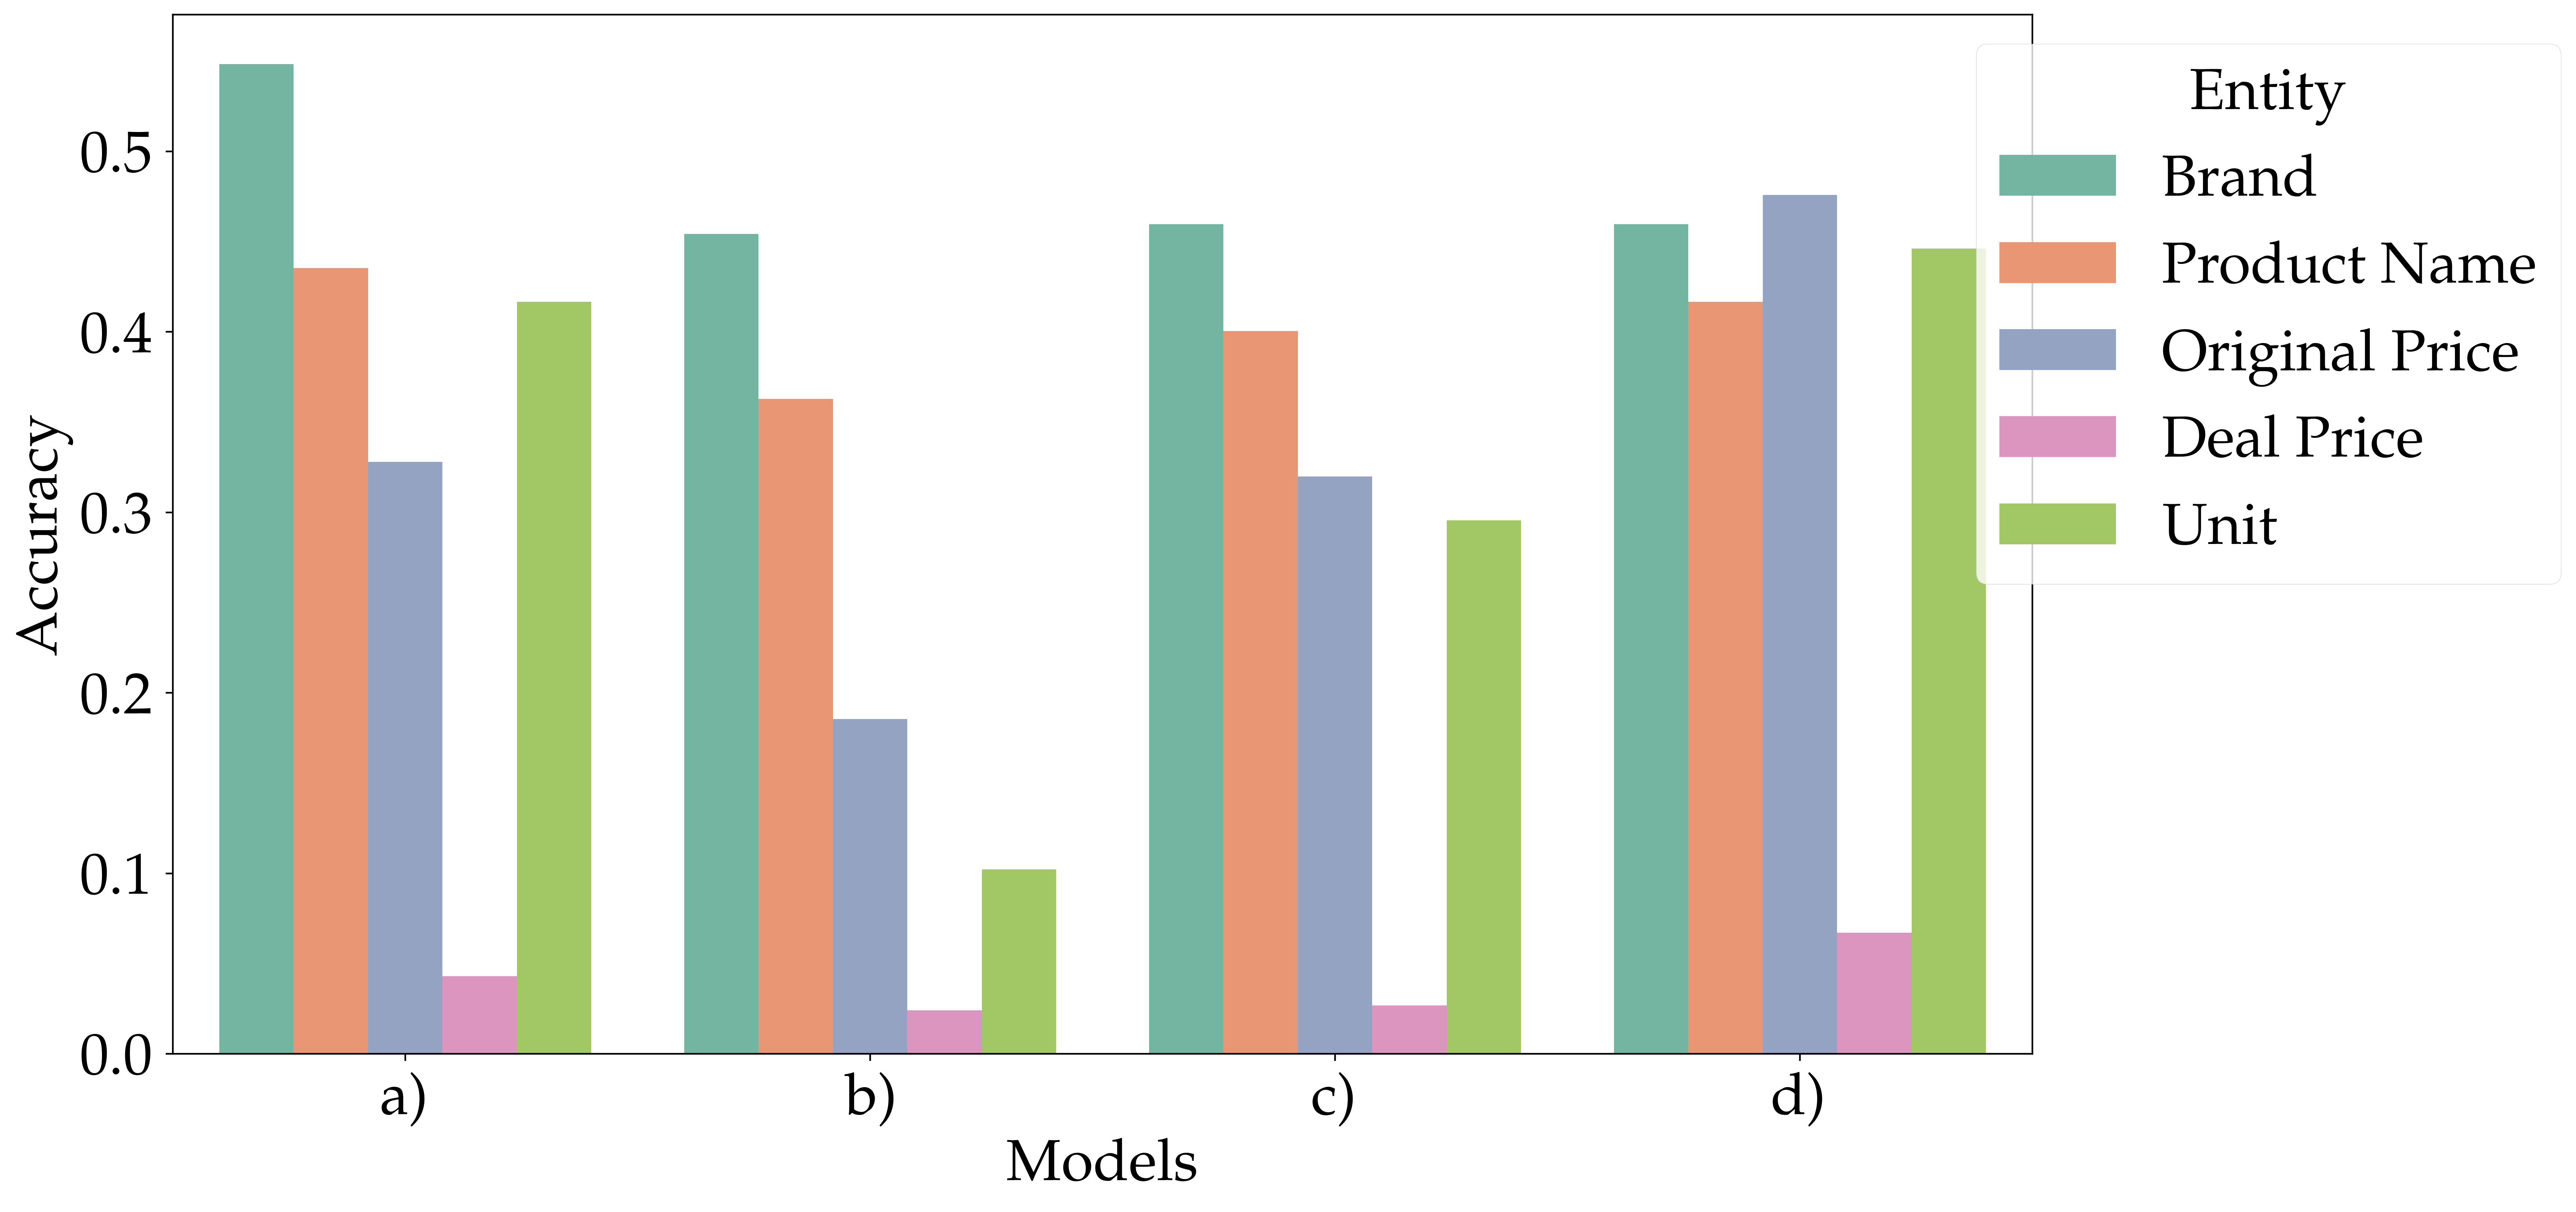
\includegraphics[width=0.5\linewidth]{figures/tesseract_ocr_accuracies.png} \\
    docTR & Tesseract \\[6pt]
        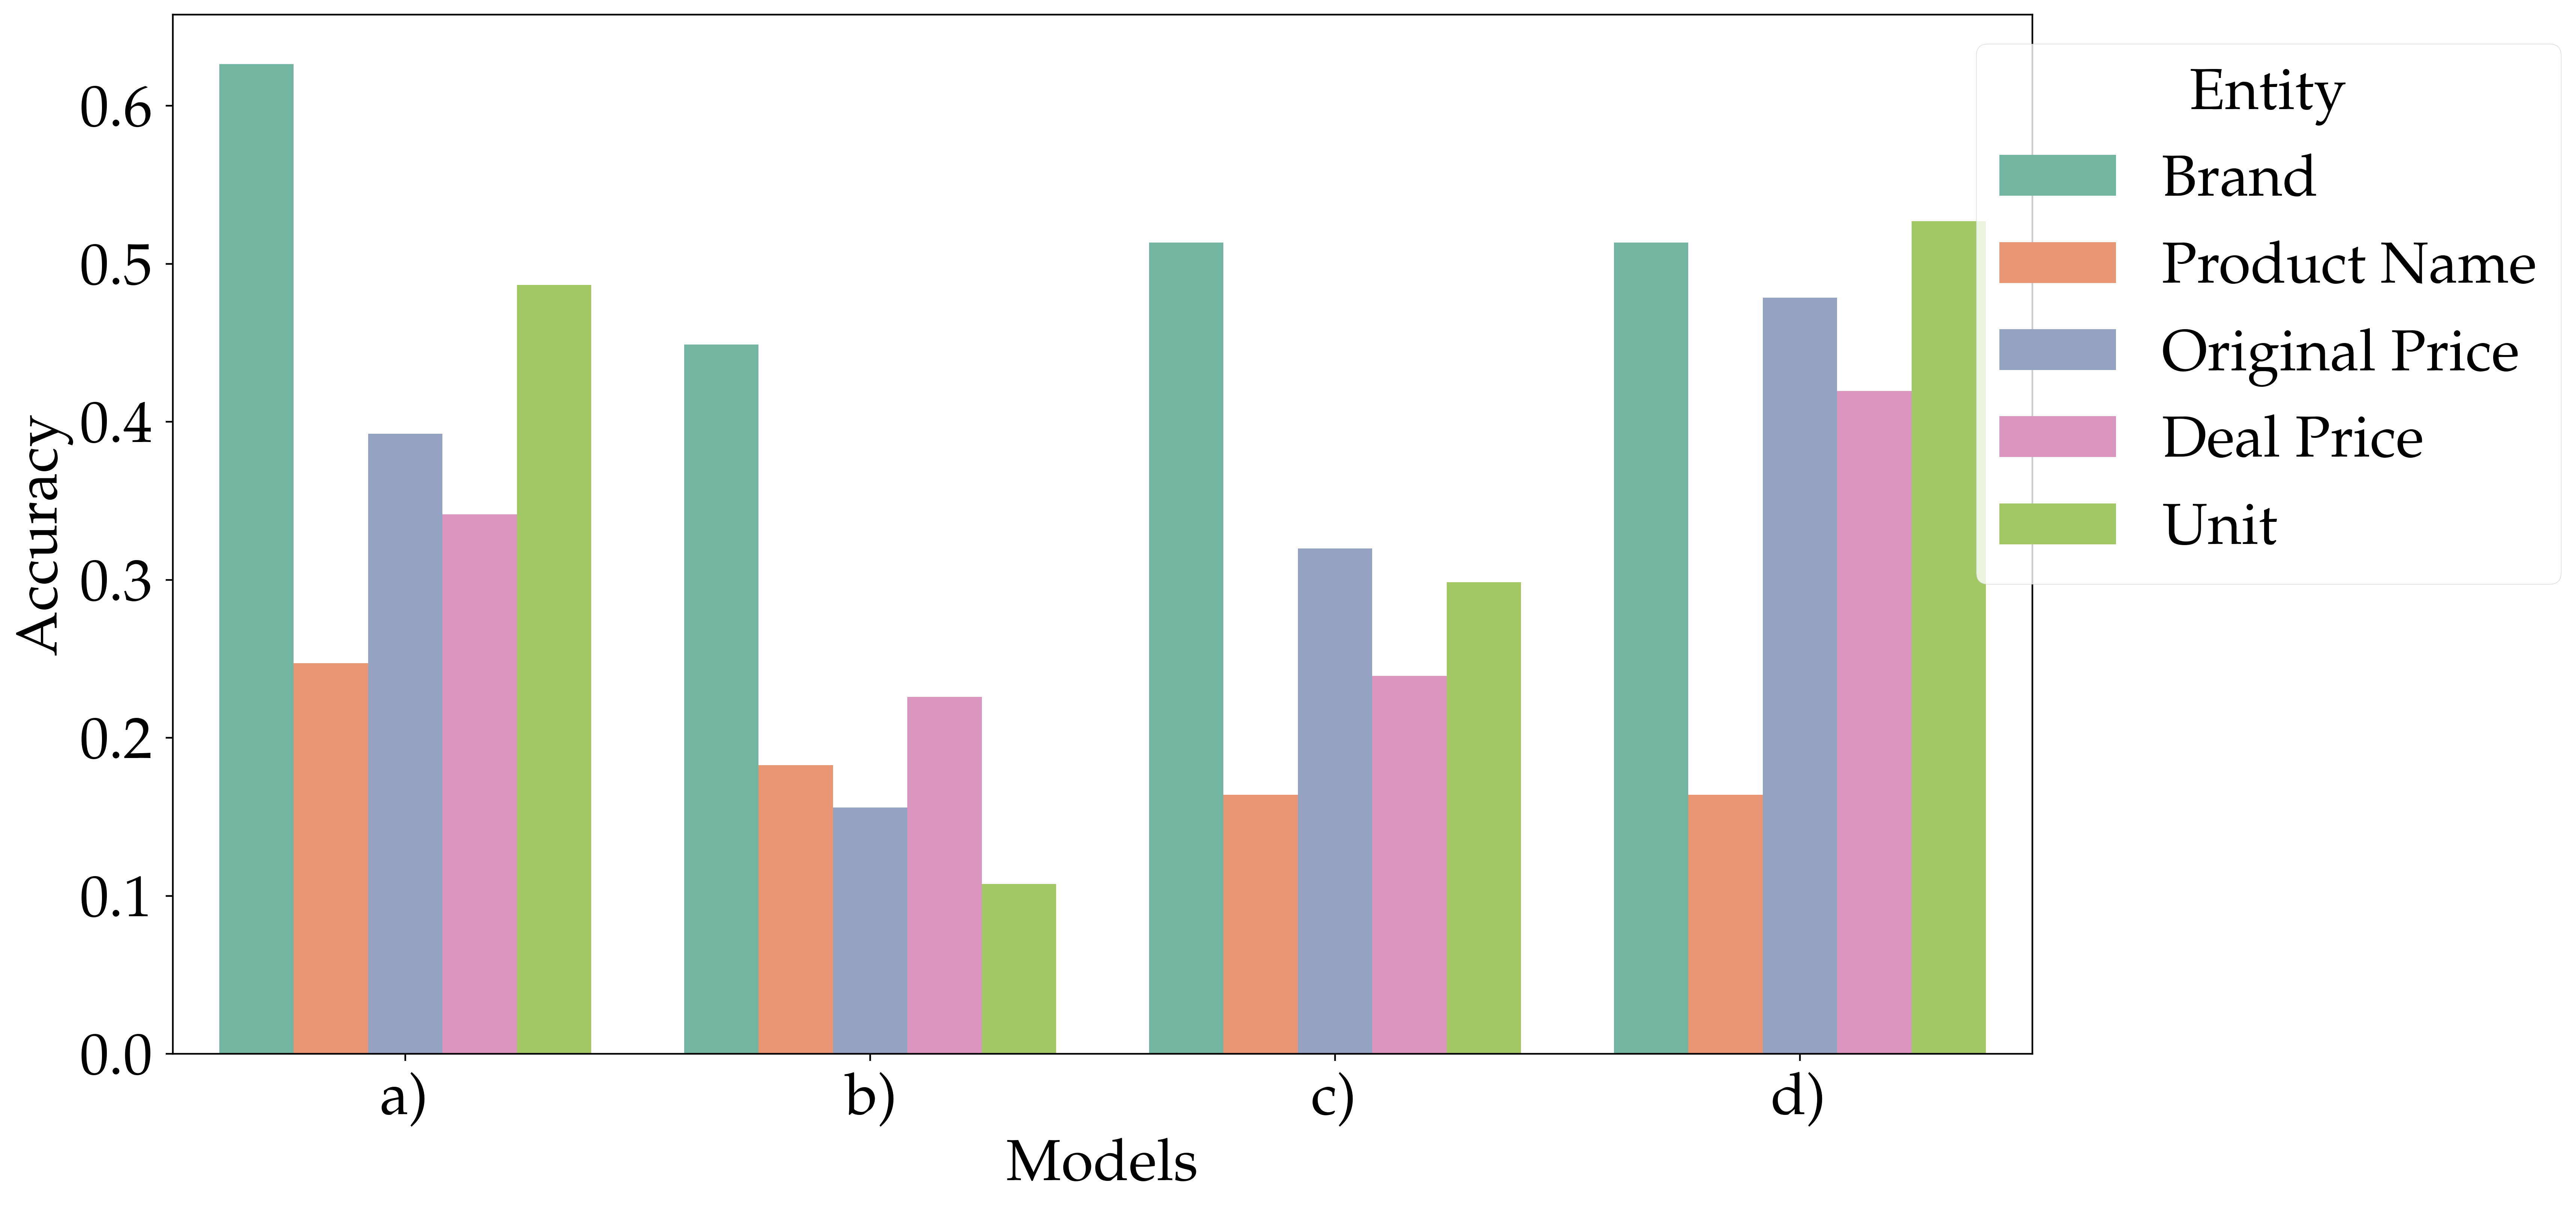
\includegraphics[width=0.5\linewidth]{figures/easyocr_ocr_accuracies.png} &   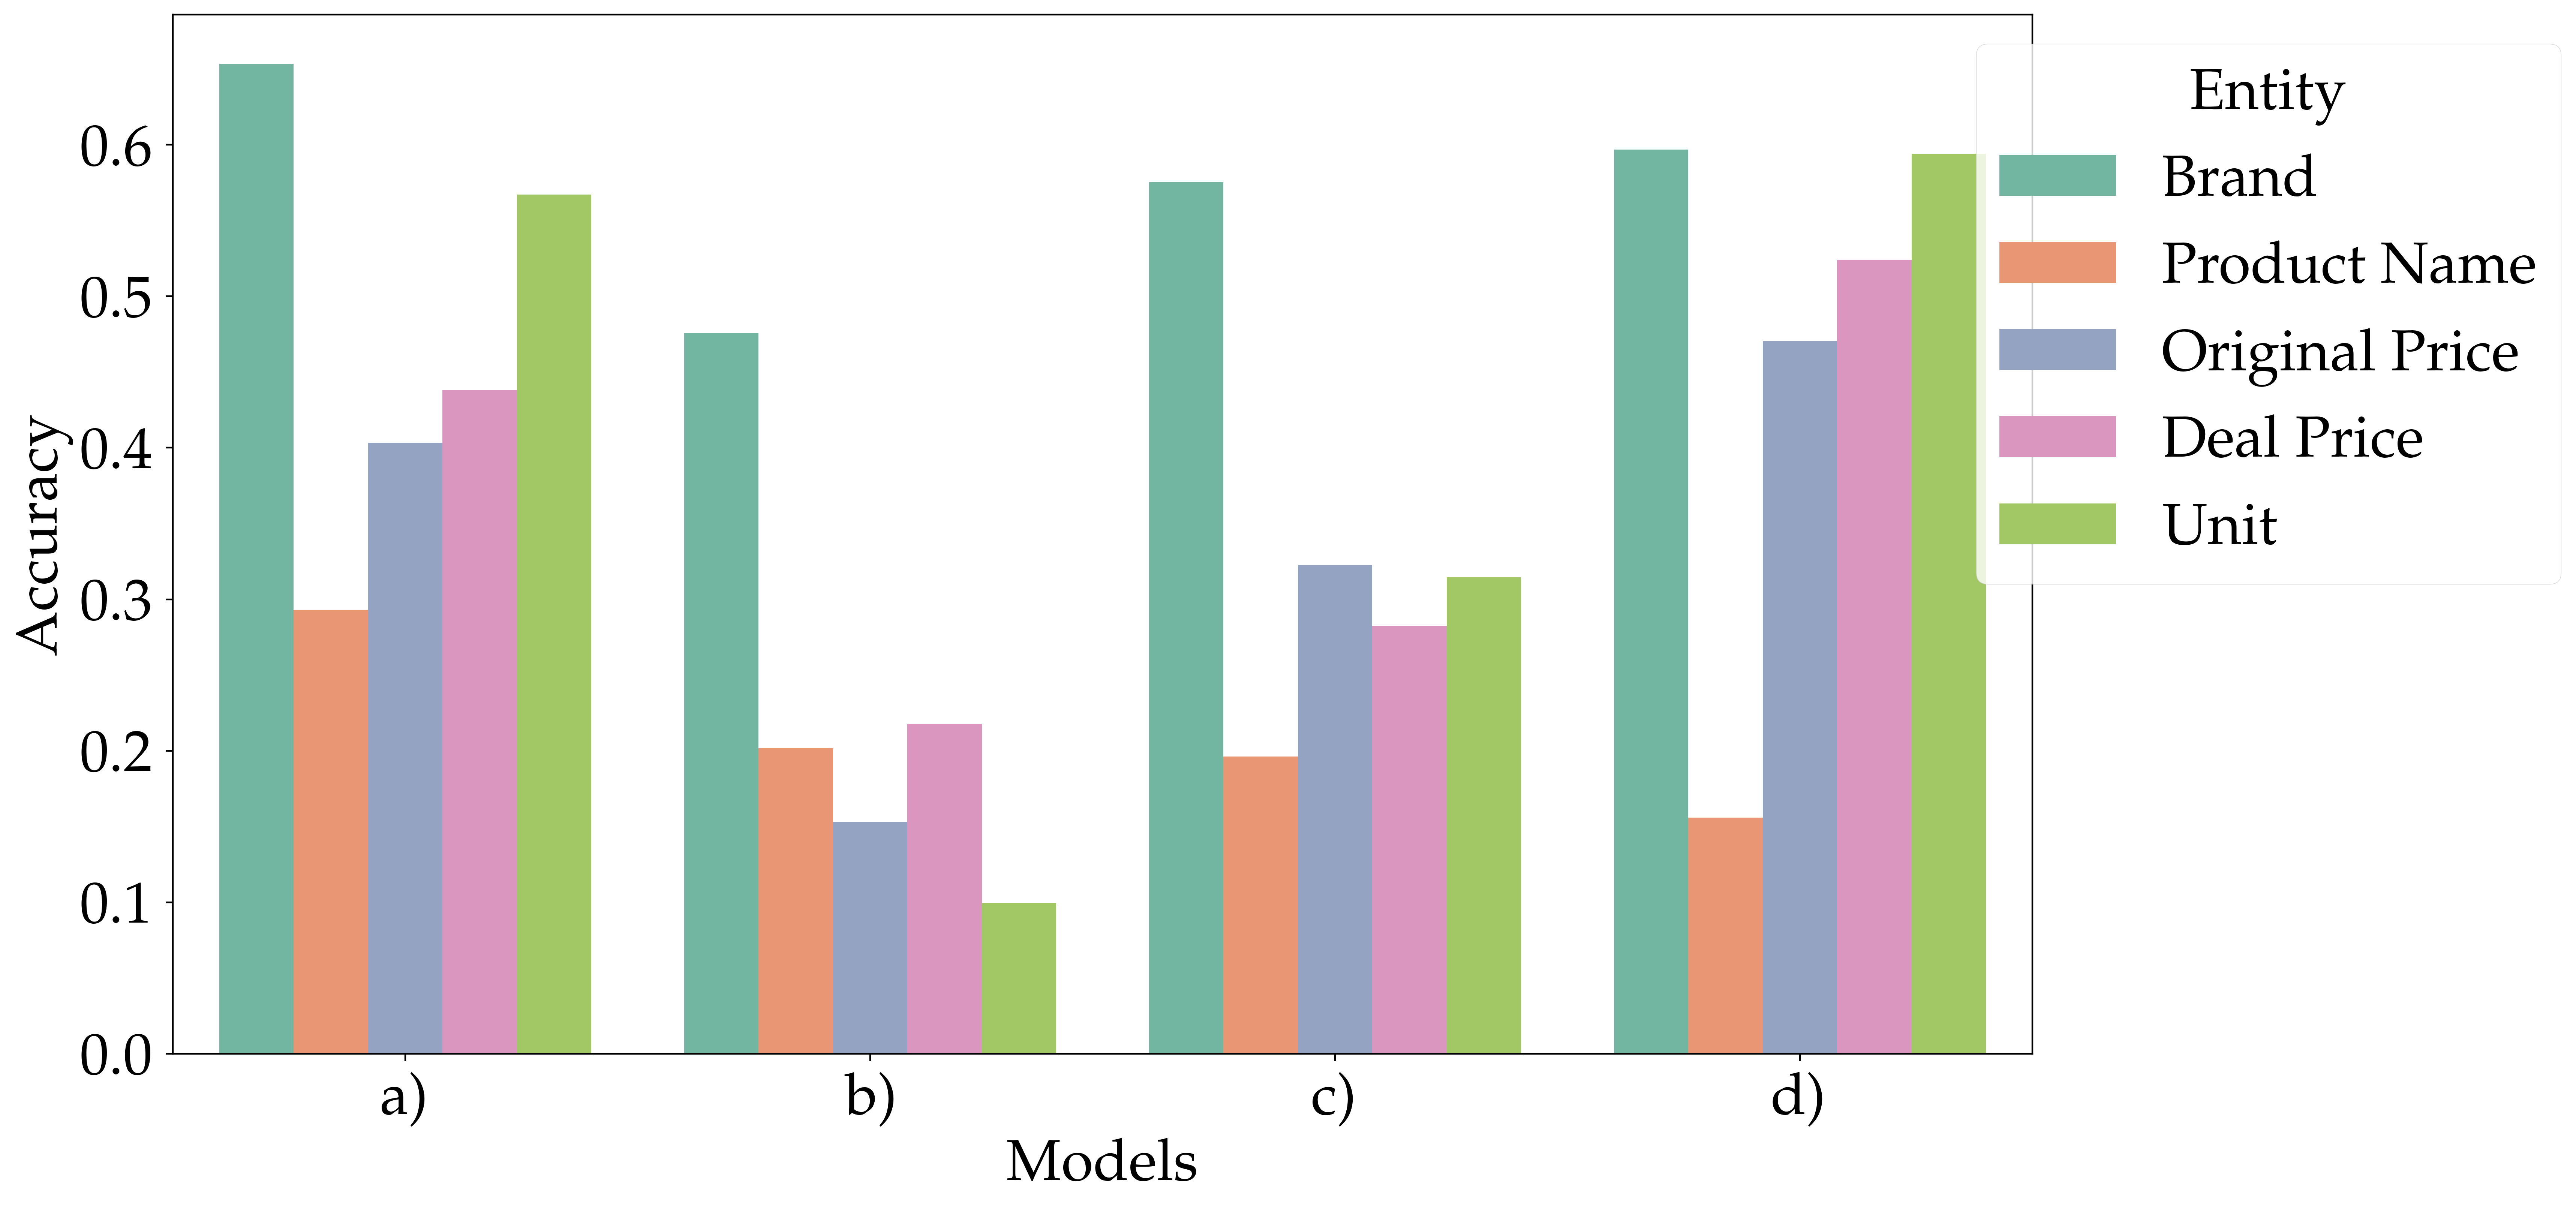
\includegraphics[width=0.5\linewidth]{figures/ppocr_ocr_accuracies.png} \\
    EasyOCR & PaddleOCR \\[6pt]
    \end{tabular}
    \caption{LLM accuracies per Entity for different OCR models. a: Llama 3.1 [8b, Q4], b: Qwen 2.5 [1.5b, Q8], c: Llama 3.2 [3b, Q8], d: Qwen 2.5 [7b, Q4].}
    \label{fig:eval_ocr_llm_accuracies}
\end{figure*}

\begin{figure*}[h!]
    \begin{tabular}{cc}
        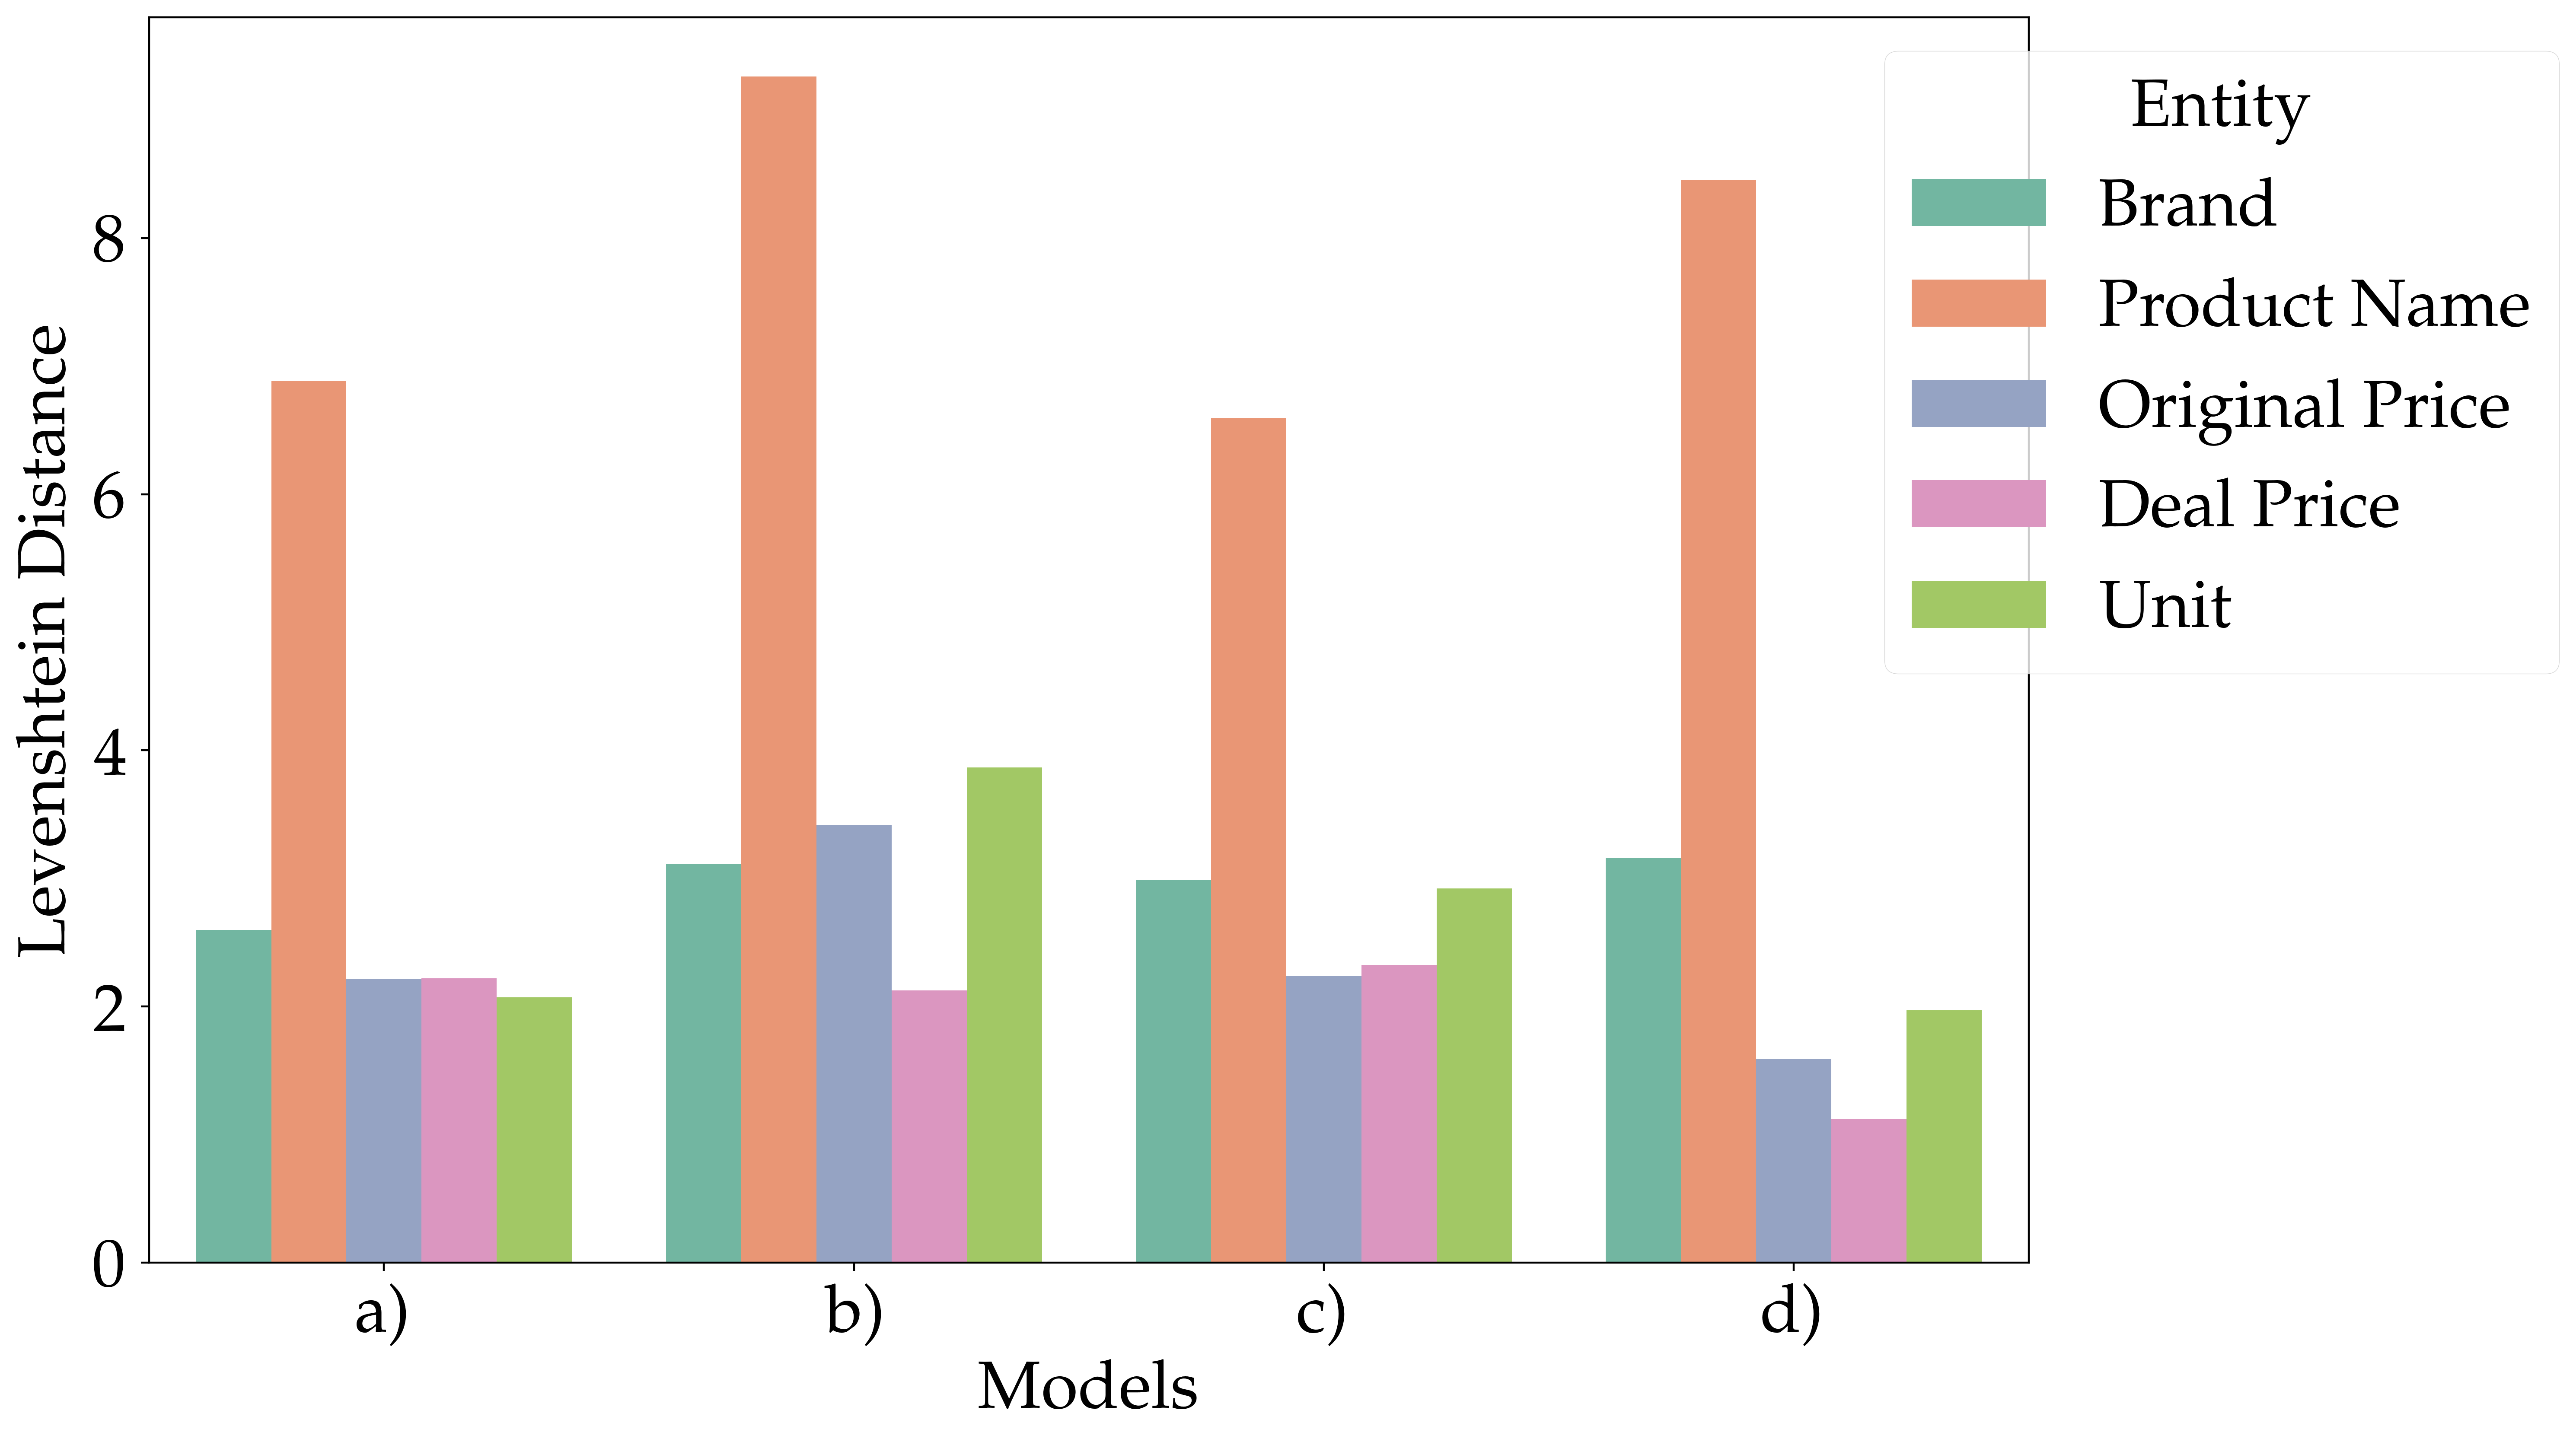
\includegraphics[width=0.5\linewidth]{figures/doctr_ocr_levdistances.png} &   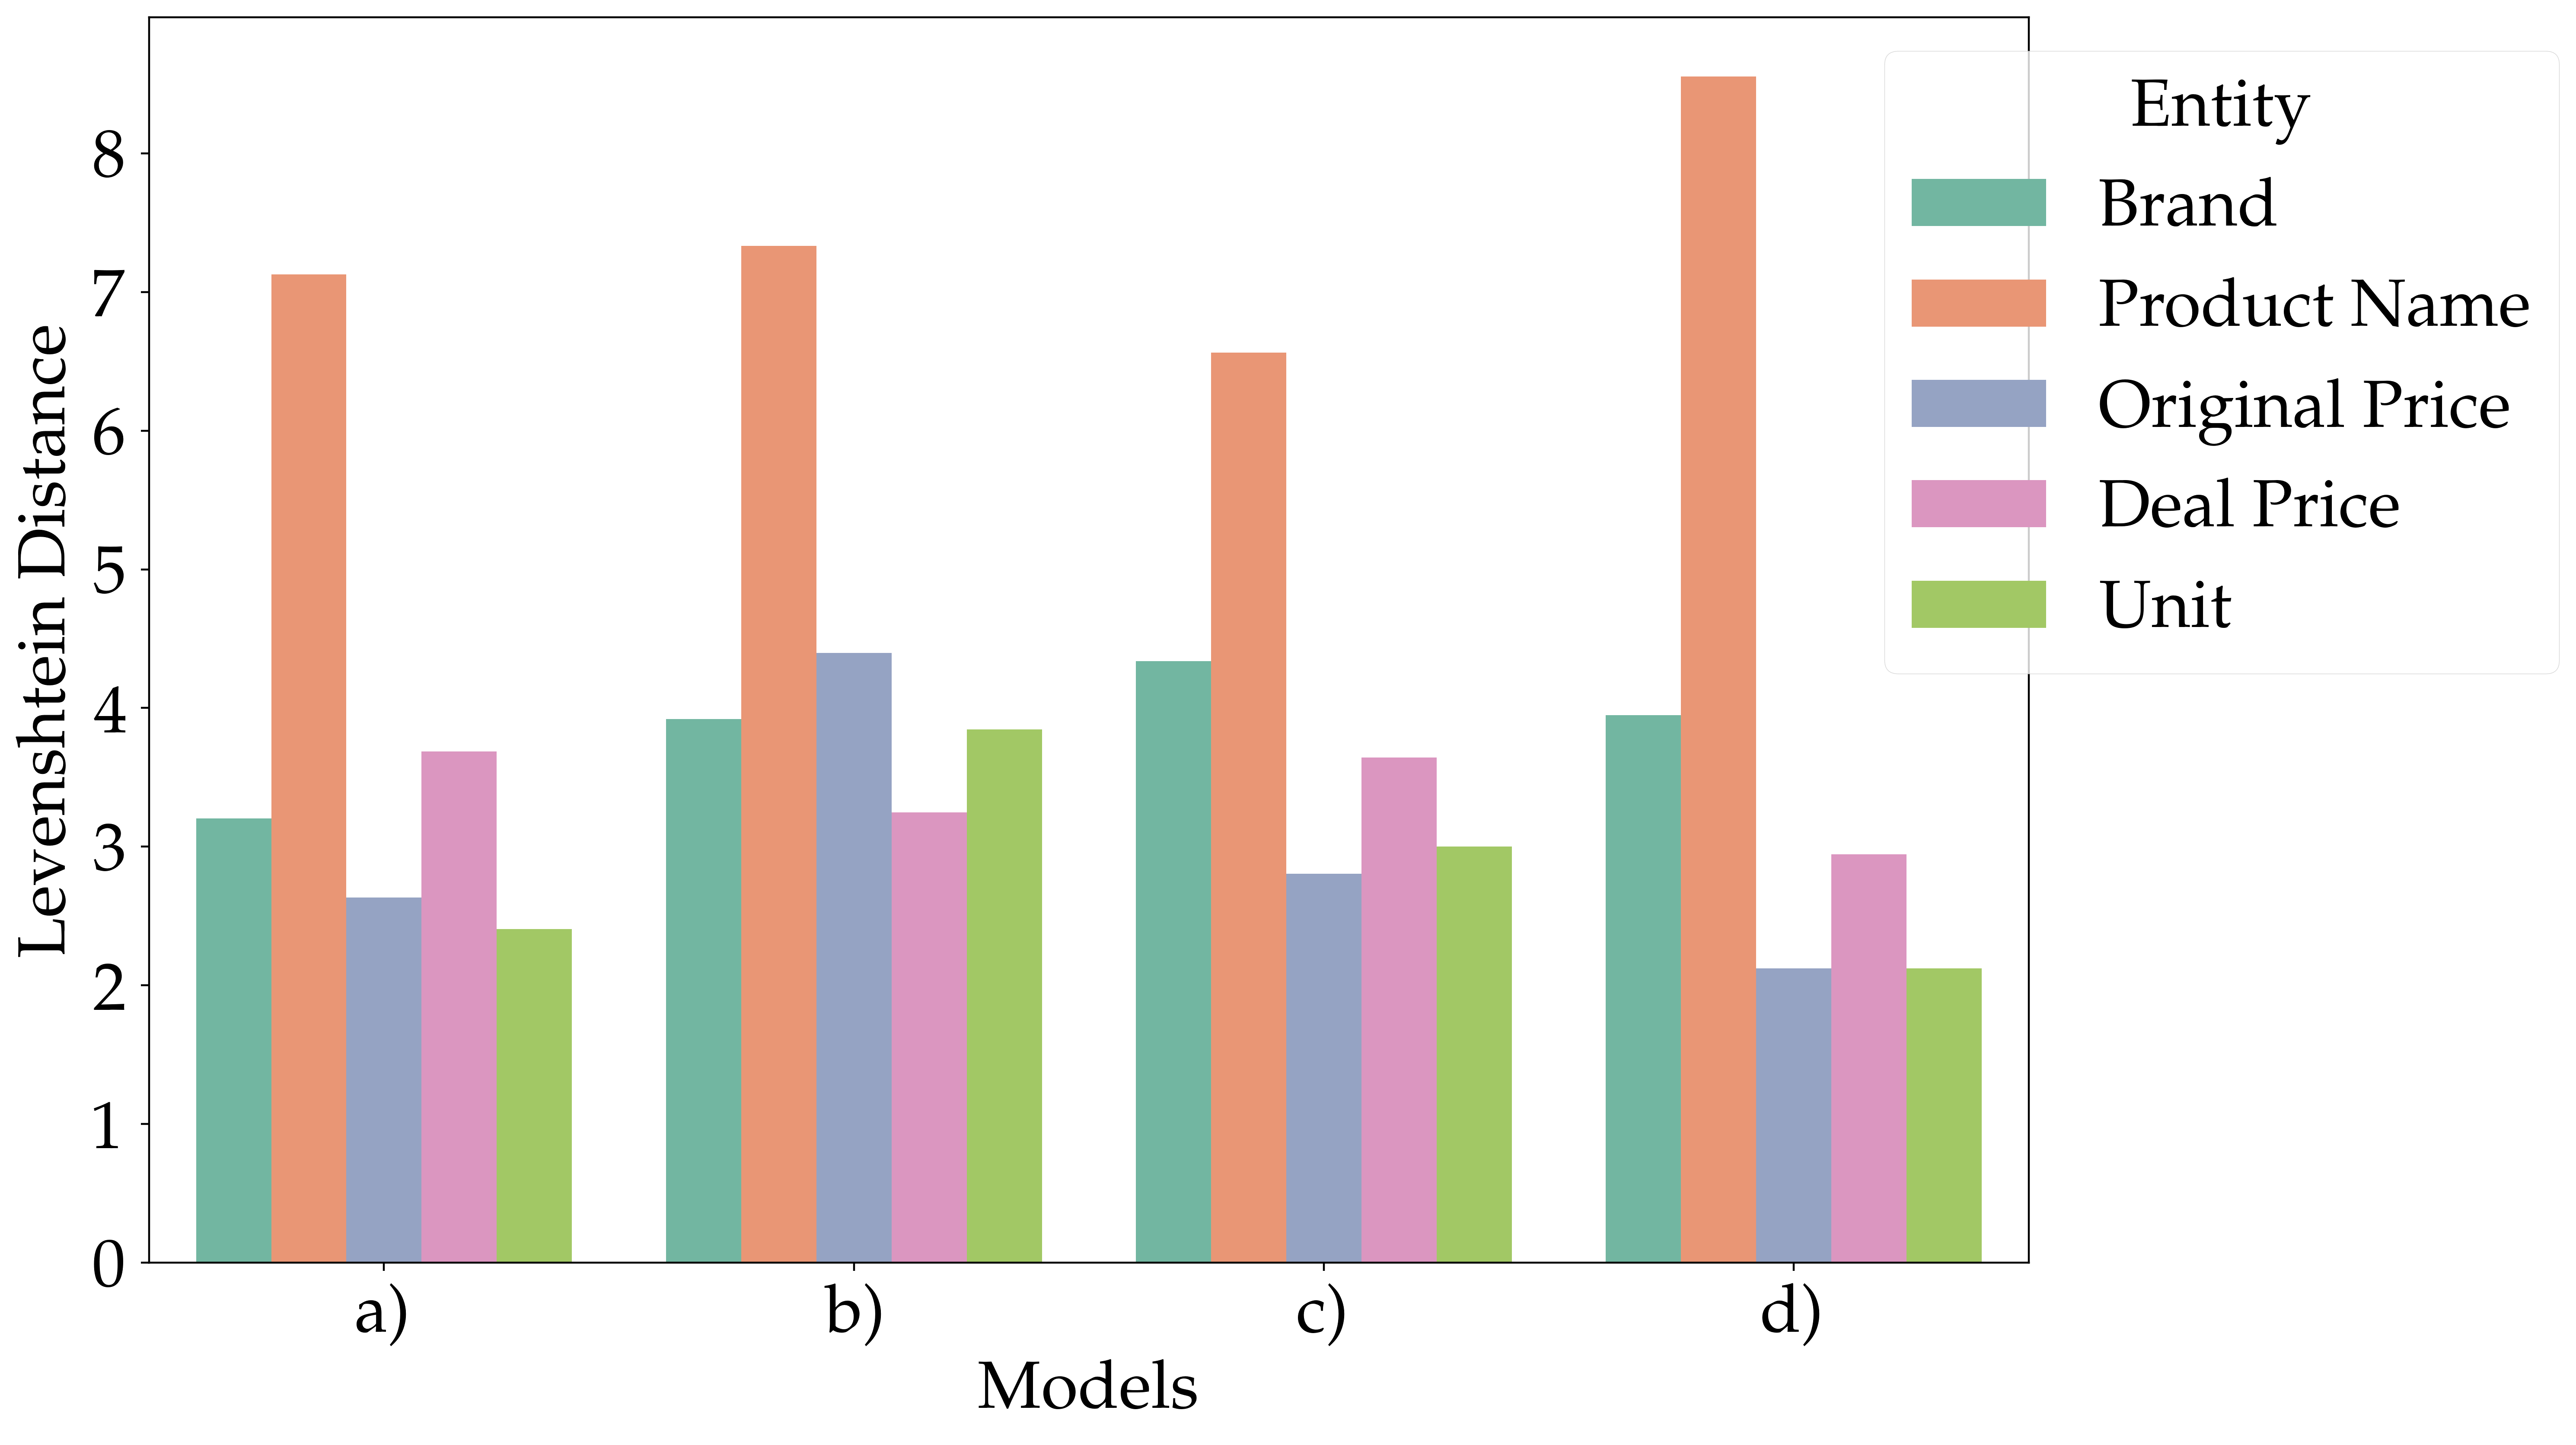
\includegraphics[width=0.5\linewidth]{figures/tesseract_ocr_levdistances.png} \\
    docTR & Tesseract \\[6pt]
        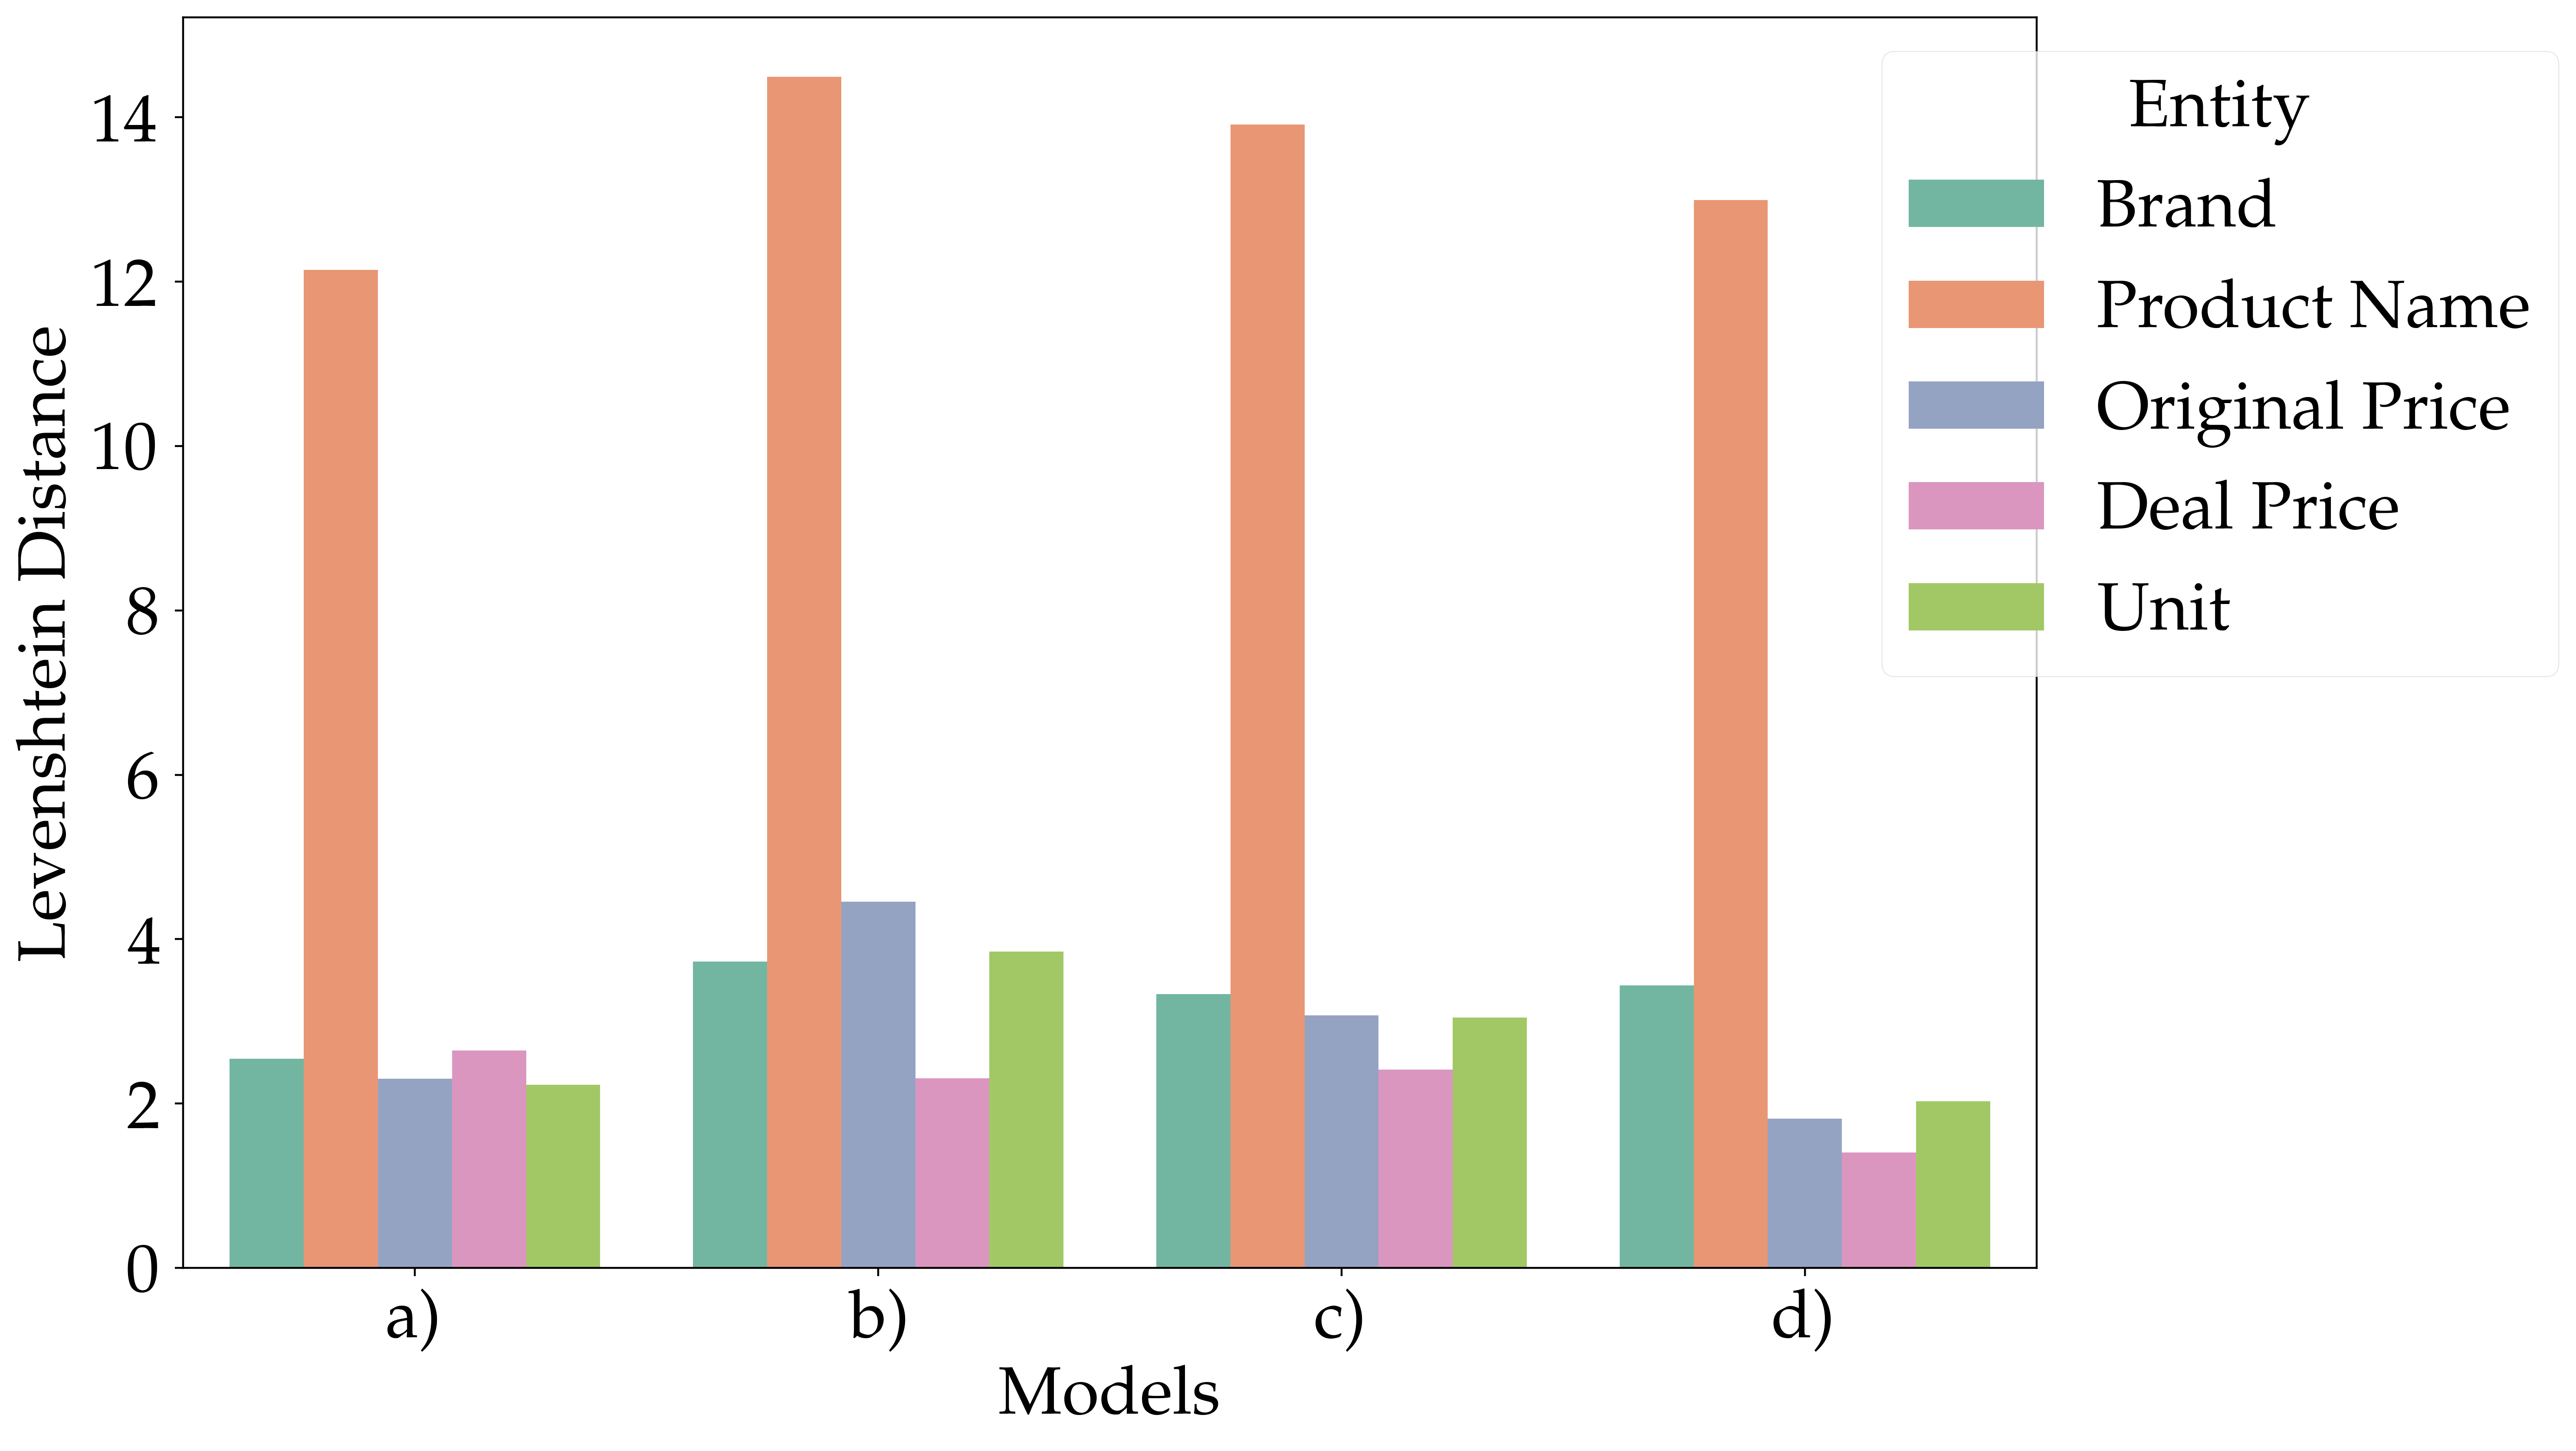
\includegraphics[width=0.5\linewidth]{figures/easyocr_ocr_levdistances.png} &   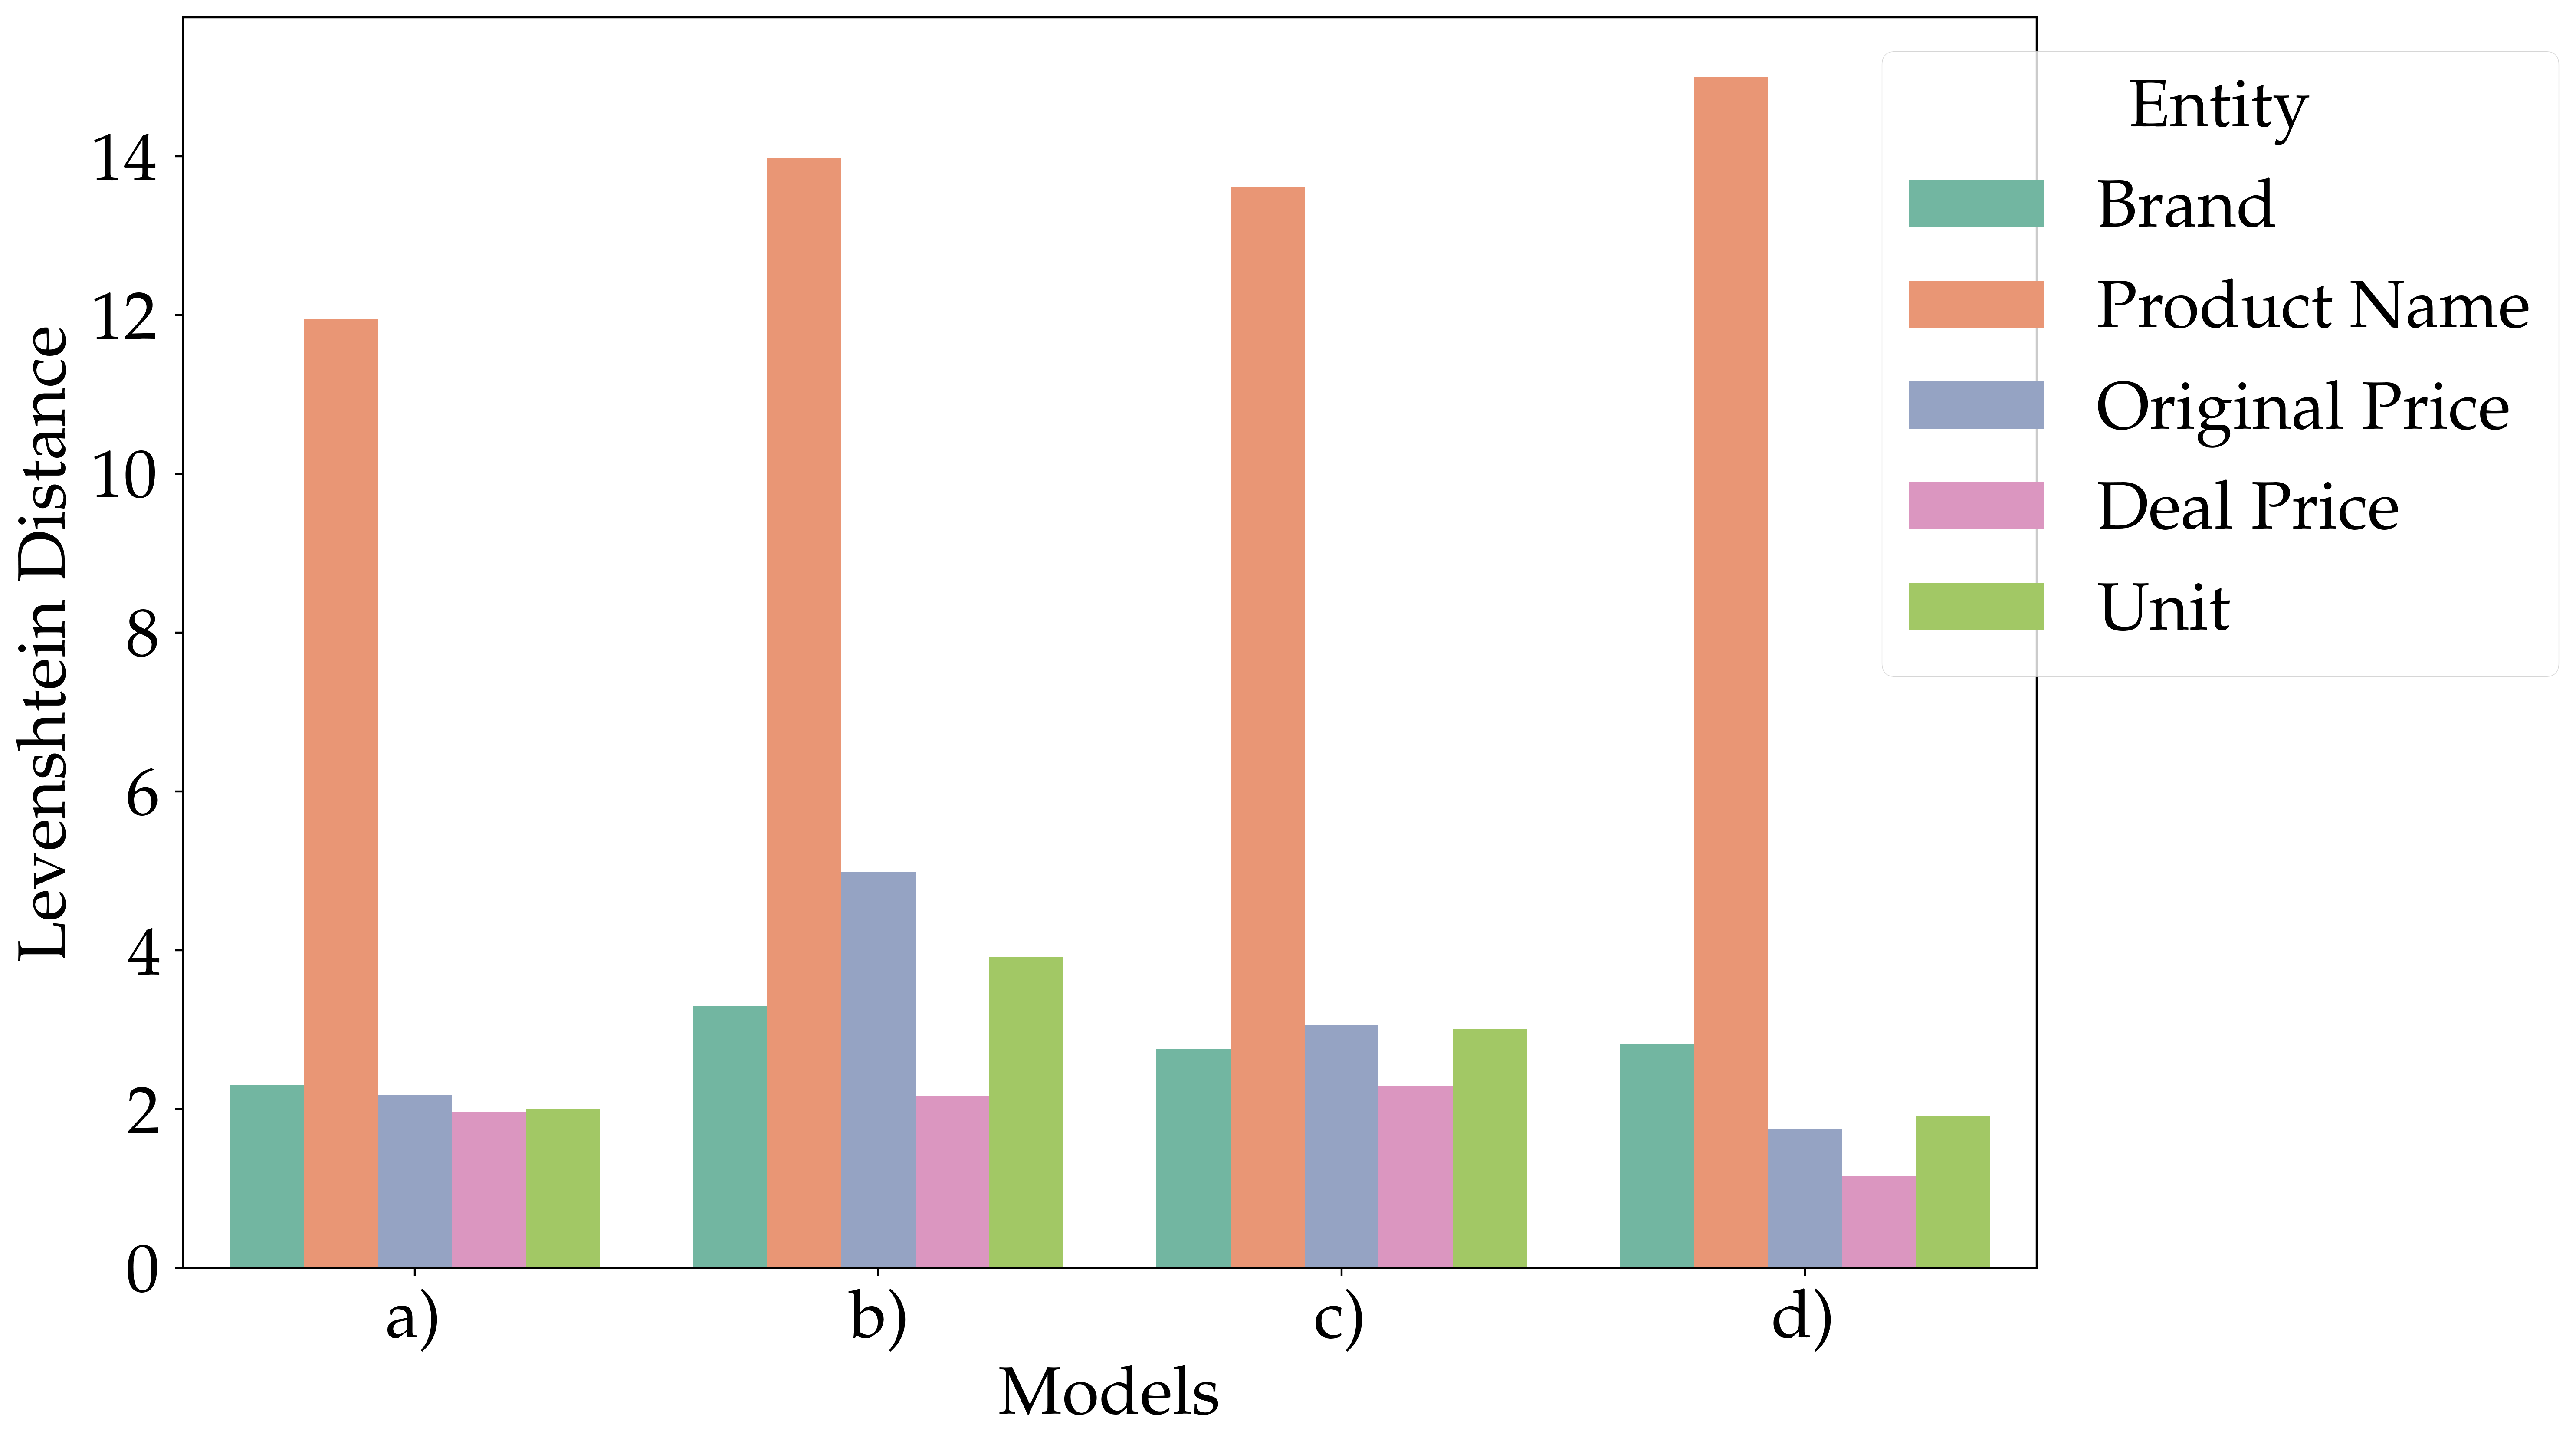
\includegraphics[width=0.5\linewidth]{figures/ppocr_ocr_levdistances.png} \\
    EasyOCR & PaddleOCR \\[6pt]
    \end{tabular}
    \caption{LLM Levenshtein Distances per Entity for different OCR models. a: Llama 3.1 [8b, Q4], b: Qwen 2.5 [1.5b, Q8], c: Llama 3.2 [3b, Q8], d: Qwen 2.5 [7b, Q4].}
    \label{fig:eval_ocr_llm_levdistances}
\end{figure*}

\end{document}